\documentclass{lib/skripsi}

\usepackage{blindtext}
\usepackage{longtable}
\usepackage{multirow}
\usepackage[table]{xcolor}
\usepackage{amsmath}  % for \hookrightarrow

%===========================================================
% Definisi Data Peneliti, Judul, Pembimbing dan Penguji
%-----------------------------------------------------------
\titleskripsi{SISTEM IDENTIFIKASI KENDARAAN PADA PEMARKIRAN DENGAN PENGENALAN CITRA PLAT DAN PEMBACAAN RFID}

\fullname{MUH FIKRI SATRIA AMDANI}
\idnum{H131 16 501}

\yearsubmit{2021}
\program{Sistem Informasi}
\dept{Matematika}
\faculty{Matematika dan Ilmu Pengetahuan Alam}
\university{Universitas Hasanuddin}
\city{Makassar}

\firstsupervisor{Dr. Eng. Armin Lawi, S.Si., M.Eng.}
\firstsupervisorNIP{19720423 199512 1 001}
\secondsupervisor{Musfira Putri Lukman, S.T., M.T.}
\secondsupervisorNIP{909048802}
\firstexaminer{ Dr. Hendra, S.Si., M.Kom.}
\secondexaminer{ Nur Hilal A Syahrir, S.Si., M.Si.}

\degree{Sarjana Komputer}
\datesubmit{14}
\monthsubmit{Desember}
\headprogram{Dr. Muhammad Hasbi, M.Sc}
\headprogramNIP{196307201989031003}
%-----------------------------------------------------------
% End Definisi Data Peneliti, Judul, Pembimbing dan Penguji
%===========================================================

\begin{document}
    % HALAMAN SAMPUL
    \cover
    \pagenumbering{roman}
    
    % HALAMAN JUDUL
    \titlepage

    % PERNYATAAN KEOTENTIKAN
    \authenticationpage

    % LEMBAR PERSETUJUAN PEMBIMBING
    \supervisorapprovalpage

    % Halaman Pengesahan
    \approvalpage

    % KATA PENGANTAR
    \addcontentsline{toc}{chapter}{KATA PENGANTAR}
    \chapter*{KATA PENGANTAR}

Segala puji dan syukur penulis panjatkan kehadirat Allah SWT, yang senantiasa melimpahkan rahmat dan karunia-Nya. Shalawat dan salam senantiasa tercurah kepada Nabi Besar Rasulullah Muhammad SAW yang telah membawa kita ke luar dari zaman kegelapan menuju zaman yang terang benderang saat ini. 

Alhamdulillah, skripsi dengan judul "\textit{SISTEM IDENTIFIKASI KENDARAAN PADA PEMARKIRAN DENGAN PENGENALAN CITRA PLAT DAN PEMBACAAN RFID}" yang disusun sebagai salah satu syarat untuk mencapai gelar Sarjana pada program studi Sistem Informasi fakultas Matematika dan Ilmu Pengetahuan Alam Universitas Hasanuddin ini dapat diselesaikan. Walaupun dalam penulisan skripsi ini sempat terkendala dengan adanya wabah Covid-19, tetapi penulis mampu menyelesaikan pada waktu yang tepat berkat bantuan dan dukungan dari berbagai pihak.

Penulis menghanturkan ungkapan hormat dan terima kasih yang tulus kepada keluarga besar penulis terkhusus bagi Ayahanda \textbf{Satu Dani} dan Ibunda \textbf{Rismawati Amir}, yang dengan penuh kesabaran dalam mengasuh dan mendidik penulis dan tak kenal lelah dalam memanjatkan doa serta memberikan nasihat dan motivasi kepada penulis. Ucapan terima kasih juga kepada saudari tercinta \textbf{Alfiyah Gemintang Ramadhani} dan \textbf{Alya Arsyi Amdani} yang senantiasa memberikan dukungan dan doa bagi penulis dalam menyelesaikan skripsi ini.

Penulis menyadari bahwa penelitian ini dapat terselesaikan dengan adanya bantuan, bimbingan, dukungan dan motivasi dari berbagai pihak. Oleh karena itu, penulis mengungkapkan ucapan terima kasih dengan tulus kepada :

\begin{enumerate}[topsep=0pt,itemsep=0pt,partopsep=0pt, parsep=0pt]
    \item Rektor Universitas Hasanuddin, Ibu \textbf{Prof. Dr. Dwia Aries Tina Pulubuhu} beserta jajarannya.
    \item Dekan Fakultas Matematika dan Ilmu Pengetahuan Alam, \textbf{Dr. Eng. Amiruddin} beserta jajarannya.
    \item Ketua Departemen Matematika FMIPA, \textbf{Dr. Nurdin, S.Si., M.Si.}, dan juga \textbf{Dr. Muhammad Hasbi, M.Sc.} sebagai ketua Program Studi Sistem Informasi Universitas Hasanuddin.
    \item Bapak \textbf{Dr. Eng. Armin Lawi, S.Si., M.Eng.} sebagai pembimbing utama yang telah banyak memberikan arahan, ide, motivavsi serta dukungan kepada penulis dalam penyelesaian skripsi.
    \item Ibu \textbf{Musfira Putri Lukman, S.T., M.T.} yang sebagai pembimbing pertama yang senantiasa memberikan masukan dan arahan kepada penulis.
    \item Bapak \textbf{Dr. Hendra, S.Si., M.Kom.} sebagai anggota tim penguji atas saran dan kritik yang membangun pada penelitian yang telah dilakukan oleh penulis.
    \item Ibu \textbf{Nur Hilal, S.Si., M.Si.} sebagai anggota tim penguji atas saran dan kritik yang membangun pada penelitian yang telah dilakukan oleh penulis.
    \item Bapak \textbf{Supri Bin Hj. Amir, S.Si., M.Eng.} sebagai dosen pembimbing akademik yang senantiasa memberikan motivasi, dorongan, dan masukan dalam hal akademik.
    \item Seluruh Bapak dan Ibu dosen FMIPA Universitas Hasanuddin yang telah mendidik dan memberikan ilmunya sehingga penulis mampu menyelesaikan program sarjana. Serta para staf yang telah membantu dalam pengurusan berkas administrasi.
    % \item Saudara-saudara \textbf{Sunu Squad} \textbf{(Sulaeman, Muhammad Akbar Atori, Nur Ikhwan Putra Pratama, Baharuddin Kasim, Andi Rezki Muh Nur, Bagas Prasetyo, Andi Yaumil Falakh, Abdul Aziz Mubarak)} yang telah menemani penulis selama perkuliahan, saling memberi motivasi dan bantuan, meluangkan waktu dan berbagi suka-duka serta kebersamaan selama menuntut ilmu.
    \item Keluarga besar \textbf{Ilmu Komputer Unhas 2016} yang setia menemani dan penulis selama menjalani pendidikan.
    \item Kakak-kakak dan Adik-adik \textbf{Ilmu Komputer 2014, 2015, 2017, 2018} yang telah banyak membantu, semoga tetap semangat dalam mengejar impian.
    \item Rekan-rekan \textbf{KKN E-Commerce Luwu Utara} yang telah menjadi keluarga baru selama KKN dan menjadikan KKN sebagai momen yang membahagiakan.
    \item Semua pihak yang telah banyak berpartisipasi, baik secara langsung maupun tidak langsung dalam penyusunan skripsi ini yang tidak sempat penulis sebutkan satu per satu.
\end{enumerate}

Penulis menyadari bahwa skripsi ini masih jauh dari sempurna dikarenakan terbatasnya pengalaman dan pengetahuan yang dimiliki penulis. Oleh karena itu, penulis mengharapkan segala bentuk saran serta masukan bahkan kritik yang membangun dari berbagai pihak. Semoga tulisan ini memberikan manfaat kepada semua pihak yang membutuhkan dan terutama untuk penulis.

\vspace{1cm}
\begin{flushright}
    Makassar, 9 September 2021\\
    \vspace{2.5cm}
    {MUH FIKRI SATRIA AMDANI}\\
    NIM. {H13116501}
\end{flushright}
    \pagebreak

    % PERNYATAAN PERSETUJUAN PUBLIKASI
    \publicationapprovalpage

    % ABSTRAK
    \addcontentsline{toc}{chapter}{ABSTRAK}
    \chapter*{ABSTRAK}

Konsep \textit{Internet of Things} sudah banyak digunakan dalam kehidupan sehari-hari di berbagai bidang, seperti bidang pertanian, bidang kesehatan, bidang industri, bidang keamanan, serta bidang transportasi. Salah satu permasalahan yang banyak dijumpai diera sekarang adalah sistem parkir yang masih menggunakan metode konvensional untuk mencatat nomor pelat kendaraan yang akan parkir. Tujuan penelitian ini adalah untuk membuat suatu sistem yang memanfaatkan teknologi \textit{Internet of Things} di bidang transportasi. Sistem yang dimaksud adalah sistem parkir otomatis yang menggunakan pembacaan RFID dan pengenalan citra plat kendaraan. \textit{Microcomputer} yang digunakan adalah Raspberry Pi dan sensor yang digunakan adalah RFID MFRC522, sensor ultrasonik HC-SR04, servo SG90, dan kamera Raspberry Pi V2. Pada penelitian ini juga menggunakan web sebagai \textit{User Interface} yang dibuat dengan bahasa pemrograman \textit{Python} dan Flask sebagai \textit{framework}nya.

Hasil penelitian yang diperoleh adalah rancangan alat dan web yang saling terintegrasi. Semua sensor yang digunakan akan dihubungkan dengan Raspberry Pi. Data yang didapat dari sensor akan disimpan ke \textit{database} dan akan ditampilkan pada web sebagai \textit{user interface}. Data yang ditampilkan adalah data \textit{id} yang diambil dari sensor RFID dan data nomor plat kendaraan yang diambil dari kamera. Sensor ultrasonik akan mengambil data jarak kendaraan dan servo berfungsi sebagai palang parkir. Web yang dibuat memiliki beberapa fitur seperti melihat slot yang terisi dan tersedia, mendaftarkan pengguna baru, menambah saldo, dan melihat informasi mengenai slot parkir.

\begin{table}[h]
    \begin{tabular}{ p{0.17\textwidth} p{0.8\textwidth} }
        \\
        \textbf{Kata Kunci :} & \textit{Internet of Things}, Sistem \textit{Smart Parking}, Raspberry Pi, Web, \textit{Database}
    \end{tabular}
\end{table}
    \pagebreak

    % ABSTRACT
    \addcontentsline{toc}{chapter}{ABSTRACT}
    \chapter*{ABSTRACT}

\textit{The concept of the Internet of Things has been widely used in everyday life in various fields, such as agriculture, health, industry, security, and transportation. One of the problems that are often encountered in today's era is the parking system that still uses conventional methods to record the license plate number of the vehicle that will be parked. The purpose of this research is to create a system that utilizes Internet of Things technology in the transportation sector. The system in question is an automatic parking system that uses RFID reading and vehicle plate image recognition. The microcomputer used is a Raspberry Pi and the sensors used are RFID MFRC522, ultrasonic sensor HC-SR04, servo SG90, and Raspberry Pi V2 camera. This research also uses the web as a User Interface which is made with the Python and Flask programming languages as the framework.}

\textit{The results obtained are the design of tools and web that are integrated with each other. All sensors used will be connected to the RaspberryPi. The data obtained from the sensor will be stored on the database and will be displayed on the web as a user interface. The data displayed is the ID data taken from the RFID sensor and the vehicle plate number data taken from the camera. The ultrasonic sensor will take vehicle distance data and the servo functions as a parking barrier. The web created has several features such as viewing filled and available slots, registering new users, adding balances, and viewing information about parking slots.}

\begin{table}[h]
    \begin{tabular}{ p{0.17\textwidth} p{0.8\textwidth} }
        \\
        \textbf{Keywords :} & \textit{Internet of Things}, \textit{Smart Parking System}, \textit{Raspberry Pi}, \textit{Web}, \textit{Database}
    \end{tabular}
\end{table}
    \pagebreak

    %===========================================================
    % Daftar isi, daftar gambar, daftar tabel
    %-----------------------------------------------------------
    \addcontentsline{toc}{chapter}{DAFTAR ISI}
    \tableofcontents
    \pagebreak

    \addcontentsline{toc}{chapter}{DAFTAR TABEL}
    \listoftables
    \pagebreak

    \addcontentsline{toc}{chapter}{DAFTAR GAMBAR}
    \listoffigures
    \pagebreak

    \addcontentsline{toc}{chapter}{DAFTAR LAMPIRAN}
    \listofappendices
    \pagebreak

    \pagenumbering{arabic}
    %-----------------------------------------------------------
    % End Daftar isi, daftar gambar, daftar tabel
    %===========================================================

    %===========================================================
    % Daftar masukan untuk Bab
    %-----------------------------------------------------------
    \chapter{PENDAHULUAN}

\section{Latar Belakang}
Revolusi Industri merupakan periode di mana terjadinya perubahan secara besar-besaran di bidang pertanian, manufaktur, tekstil dan logam, pertambangan, transportasi, teknologi, dan sosial ekonomi \thecite{azli2017a}. Pada abad ke-18, mesin uap pertama ditemukan di Inggris. Mesin uap tersebut digunakan sebagai alat tenun mekanis pertama yang dapat meningkatkan produktivitas industri tekstil. Saat itu mesin uap mulai menggantikan peralatan kerja yang awalnya bergantung pada tenaga manusia dan hewan sekaligus memulai era revolusi industri pertama yang dikenal dengan Revolusi Industri 1.0. Revolusi industri kedua ditandai dengan penemuan tenaga listrik pada awal abad ke-20. Revolusi industri ketiga ditandai oleh mesin yang dapat bergerak dan berpikir secara otomatis, yaitu komputer dan robot \thecite{rahayu2019a}. 

Di abad ke-21 revolusi industry telah masuk ke era baru. Yakni telah berada pada revolusi industri keempat atau lebih dikenal dengan Revolusi Industri 4.0. Era ini telah mengubah banyak bidang kehidupan manusia, termasuk ekonomi, dunia kerja, bahkan gaya hidup. Revolusi industri 4.0 menawarkan teknologi cerdas yang dapat terhubung dengan berbagai bidang kehidupan manusia. Revolusi industri 4.0 menerapkan \textit{Internet of Things} \textit{(IoT)} dan teknologi pada kegiatan analisis, manufaktur, robotik, komputasi canggih, \textit{artificial intellegence}, teknologi, kognitif, \textit{advance materials} dan \textit{augmented reality} dalam melaksanakan siklus operasi bisnis \thecite{suharman2019a}. Saat ini negara-negara di dunia mulai berkopetisi dalam pemanfaatan teknologi pada setiap sektor industrinya. Lalu bagaimana dengan indonesia ? Mempelajari konsep industri 4.0 untuk penerapannya di Indonesia menjadi suatu keharusan, sebab jika tidak maka industry dan manufaktur di Indonesia tidak akan dapat bersaing dengan industry dan manufaktur di negara-negara lain di dunia.

Revolusi industri 4.0 mencakup beragam teknologi canggih, seperti kecerdasan buatan (AI), \textit{wearables}, robotika canggih, \textit{3D printing}, dan \textit{Internet of Things} \textit{(IoT)}. \textit{Internet of Things} \textit{(IoT)} adalah sekenario dari suatu objek yang dapat melakukan pengiriman data/informasi melalui jaringan tanpa campur tangan manusia \thecite{limantara2017a}. Konsep \textit{Internet of Things} sudah banyak digunakan dalam kehidupan sehari-hari di berbagai bidang, seperti bidang pertanian, bidang kesehatan, bidang industri, bidang keamanan, serta bidang transportasi.

Salah satu permasalahan yang banyak dijumpai diera sekarang adalah sistem parkir yang masih menggunakan metode konvensional untuk mencatat nomor pelat kendaraan yang akan parkir dan pembayaran yang masih menggunakan uang cash. Hal ini dapat memicu kemacetan, polusi udara dan suara, dan menambah tingkat stress pengendara. Untuk mengatasi masalah tersebut, dibuatlah suatu sistem dengan memanfaatkana konsep \textit{Internet of Things} di bidang transportasi dan keamanan. Sistem yang dimaksud adalah sistem parkir otomatis yang diletakkan di tempat khusus seperti di apartemen atau di perkantoran.

Salah satu aspek dalam sistem parkir otomatis adalah identifikasi citra pelat kendaraan untuk mendapatkan data nomor pelat tanpa campur tangan manusia. Identifikasi pelat kendaraan pada sistem parkir otomatis dapat dilakukan dengan kartu RFID dan pengolahan citra pelat kendaraan. Kemampuan RFID sebagai media pengenal secara nirkabel membuat RFID sering digunakan sebagai otorisasi untuk akses ruangan dan tempat, akan tetapi penggunaan RFID masih rentan terhadap keamanan akses. Penelitian ini menggabungkan identifikasi kartu RFID dan pembacaan citra pelat kendaraan sehingga dapat meningkatkan keamanan parkir dan dapat mempersingkat waktu pencatatan nomor pelat kendaraan yang masih bersifat konvensional.

\section{Rumusan Masalah}
Berdasarkan uraian pada latar belakang masalah diatas, dapat dikemukakan pertanyaan penelitian sebagai berikut:
\begin{enumerate}[topsep=0pt,itemsep=0pt,partopsep=0pt, parsep=0pt]
    \item Bagaimana cara merancang dan membangun sistem identifikasi kendaraan dengan pengenalan citra pelat dan pembacaan RFID ?
    % \item Bagaimana cara membuat aplikasi web untuk memantau situasi lahan parkir ?
    \item Bagaimana cara membuat aplikasi web sebagai \textit{user interface} sistem parkir ?
\end{enumerate}

\section{Tujuan Penelitian}
Berdasarkan rumusan masalah, maka tujuan penelitian ini adalah :
\begin{enumerate}[topsep=0pt,itemsep=0pt,partopsep=0pt, parsep=0pt]
    \item Merancang sistem identifikasi kendaraan dengan pengenalan citra pelat dan pembacaan RFID. 
    \item Membuat aplikasi web sebagai \textit{user interface}.
    % \item Menghubungkan sistem parkir dengan web yang dibuat sebagai \textit{user interface}.
\end{enumerate}

\section{Batasan Masalah}
Batasan masalah pada penelitian ini adalah :
\begin{enumerate}[topsep=0pt,itemsep=0pt,partopsep=0pt, parsep=0pt]
    \item Alat yang dibuat bersifat prototype.
    \item Sistem parkir yang dibuat ditujukan untuk diterapkan di lingkungan berpenghuni tetap seperti apartemen atau perkantoran.
    \item Karakter pada pelat nomor harus sesuai dengan yang digunakan Samsat.
    \item Tidak melakukan analisis lebih lanjut pada deteksi nomor pelat kendaraan.
\end{enumerate}

\section{Manfaat Penelitian}
Hasil penelitian ini diharapkan dapat bermanfaat :
\begin{enumerate}[topsep=0pt,itemsep=0pt,partopsep=0pt, parsep=0pt]
    \item Menghemat waktu dan bahan bakar.
    \item Terciptanya alat yang dapat menopang kemajuan industri.
    \item Mengurangi antrian Panjang yang disebabkan oleh pencatatan nomor pelat dan pembayaran parkir yang masih konvensional.
    \item Mempermudah pengelolah parkir untuk memantau sisa kapasitas lahan parkir yang tersedia.
    \item Membantu upaya pemerintah dalam pembangunan \textit{smart city} di Indonesia.
\end{enumerate}


    \chapter{TINJAUAN PUSTAKA}

\section{Internet of Things (IOT)}
\begin{afigure} 
    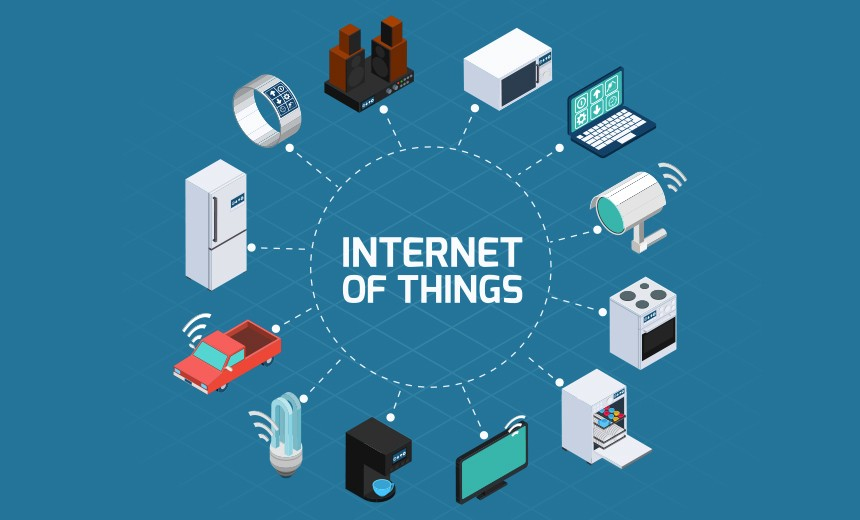
\includegraphics[width=0.85\textwidth, center]{images/iot.jpeg}
    \caption{Internet of Things}
    \label{fig:iot}
\end{afigure}

\textit{Internet of Things} adalah skenario dari suatu objek yang dapat melakukan suatu pengiriman data/informasi melalui jaringan tanpa campur tangan manusia. \textit{IoT} sangat erat hubungannya dengan komunikasi mesin ke mesin (M2M) tanpa campur tangan manusia ataupun komputer yang lebih dikenal dengan istilah cerdas \textit{(smart)} \thecite{limantara2017a}.

Cara Kerja \textit{Internet of Things} yaitu dengan memanfaatkan sebuah argumentasi pemrograman yang dimana tiap-tiap perintah argumennya itu menghasilkan sebuah interaksi antara sesama mesin yang terhubung secara otomatis tanpa campur tangan manusia dan dalam jarak berapa pun. Internetlah yang menjadi penghubung di antara kedua interaksi mesin tersebut, sementara manusia hanya bertugas sebagai pengatur dan pengawas bekerjanya alat tersebut secara langsung.Tantangan terbesar dalam mengkonfigurasi \textit{Internet of Things} ialah menyusun jaringan komunikasinya sendiri, yang dimana jaringan tersebut sangatlah kompleks, dan memerlukan sistem keamanan yang ketat. Selain itu biaya yang mahal sering menjadi penyebab kegagalan yang berujung pada gagalnya produksi.

Metode yang digunakan oleh \textit{Internet of Things} adalah nirkabel atau pengendalian secara otomatis tanpa mengenal jarak. Pengimplementasian \textit{Internet of Things} sendiri biasanya selalu mengikuti keinginan si developer dalam mengembangkan sebuah aplikasi yang ia ciptakan, apabila aplikasinya itu diciptakan guna membantu monitoring sebuah ruangan maka pengimplementasian \textit{Internet of Things} itu sendiri harus mengikuti alur diagram pemrograman mengenai sensor dalam sebuah rumah, berapa jauh jarak agar ruangan dapat dikontrol, dan kecepatan jaringan internet yang digunakan

Banyak manfaat yang didapatkan dari \textit{Internet of Things}. Pekerjaan yang kita lakukan menjadi cepat, mudah, dan efisien. Kemunculan \textit{Internet Of Things} \textit{(IoT)} memungkinkan perangkat komputer secara otomatis dapat melakukan kontrol terhadap suatu sistem dan memungkinkan pula untuk memberi aksi ke sistem terhadap kejadian yang terjadi pada sistem yang dikontrol secara realtime \thecite{ichwana2018a}.

\section{Automatic License Plate Recognition (ALPR)}
\textit{Automatic License Plate Recognition} adalah teknologi yang menggunakan pengenalan karakter pada gambar untuk membaca plat registrasi kendaraan. ALPR digunakan oleh polisi di beberapa negara di dunia untuk tujuan penegakan hukum, termasuk untuk memeriksa apakah kendaraan terdaftar atau tidak.

Pengenalan plat nomor otomatis dapat digunakan untuk menyimpan gambar yang diambil oleh kamera serta teks dari plat nomor. Umumnya sistem menggunakan pencahayaan inframerah untuk memungkinkan kamera mengambil gambar kapan saja, siang atau malam hari. Selain itu, teknologi ALPR juga harus memperhitungkan variasi nomor plat dari suatu negara karena bentuk dan ukuran nomor plat di satu negara dengan negara lainnya kemungkinan sangat berbeda.

ALPR menjadi tren baru dalam otomatisasi sistem transportasi. Pencatatan pelat nomor kendaraan bisa dilakukan tanpa campur tangan manusia. Meskipun teknologi tersebut telah ditetapkan di negara-negara maju, negara-negara berkembang seperti Indonesia belum menerapkan teknologi tersebut karena berbagai alasan \thecite{budianto2018a}.

\section{Raspberry Pi}
Raspberry Pi adalah komputer mini yang dirancang dan diproduksi di Inggris dengan tujuan awal untuk menyediakan perangkat komputasi yang murah untuk pendidikan. Raspberry Pi ditemukan pertama kali di University of Cambridge laboratory pada tahun 2006. Raspberry Pi dirilis secara komersial pada februari 2012. Sejak saat itu \textit{board} Raspberry Pi telah melalui sejumlah revisi dan tersedia dalam 2 model yaitu model A dan model B \thecite{wicaksono2018a}.

Secara kasar ditengah semua model Raspberry Pi terdapat sebuah semikonduktor persegi atau yang dikenal sebagai \textit{integrated circuit} atau \textit{chip}. \textit{Integrated Circuit} adalah \textit{sistem-on-chip} modul yang menyediakan kemampuan untuk pemrosesan umum \textit{(general purpose)}, render grafis, dan \textit{input/output} \thecite{wicaksono2018a}.

\begin{afigure} 
    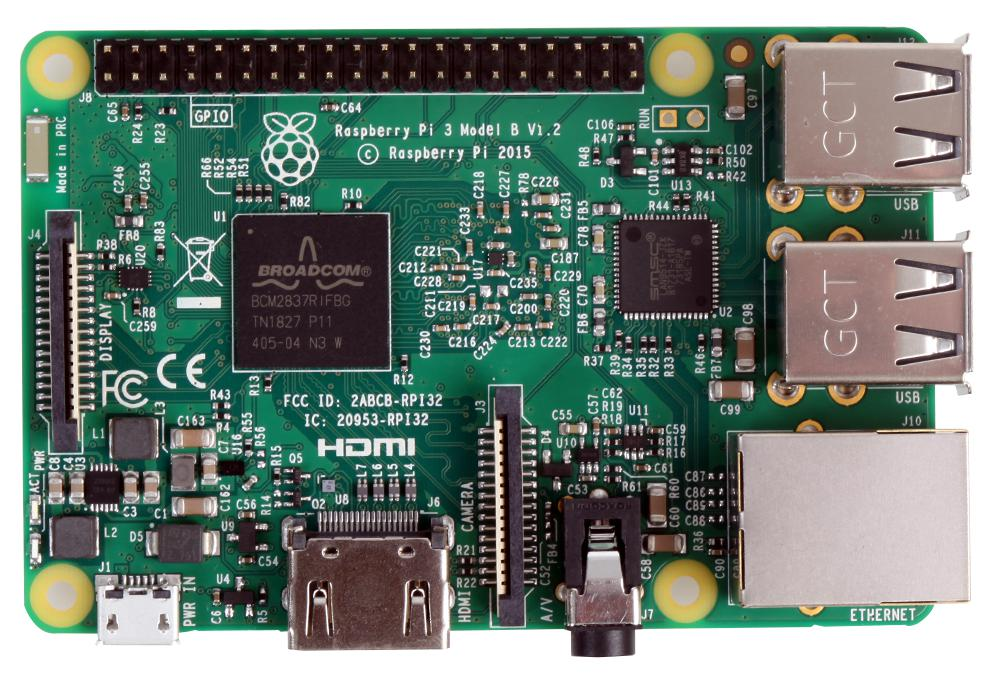
\includegraphics[width=0.85\textwidth, center]{images/raspberry pi 3b.jpg}
    \caption{Raspberry Pi model 3B}
    \label{fig:Raspberry3B}
\end{afigure}

Raspberry pi 3 adalah model terbaru Raspberry Pi. Raspberry Pi 3 menggunakan \textit{processor} terbaru yaitu Broadcom BCM283764 bit. BCM283764 lebih cepat dari pada BCM2836. Raspberry Pi 3 juga merupakan model pertama yang memiliki \textit{built-in wireless} (mampu terhubung ke jaringan WIFI dan juga memiliki perangkat \textit{Bluetooth}). Raspberry Pi model 3B bisa dilihat pada gambar ~\ref{fig:Raspberry3B}. Berikut merupakan spesifikasi dari Raspberry Pi 3 :

\begin{itemize}[topsep=0pt,itemsep=0pt,partopsep=0pt, parsep=0pt,]
    \item SoC: Broadcom BCM2837
    \item CPU: 4x ARM Cortex-A53, 1.2GHz
    \item GPU: Broadcom VideoCore IV
    \item RAM: 1GB LPDDR2 (900 MHz)
    \item Networking: 10/100 Ethernet, 2.4GHz 802.11n wireless
    \item Bluetooth: Bluetooth 4.1 Classic, Bluetooth Low Energy
    \item Storage: microSD
    \item GPIO: 40-pin header
    \item Ports: HDMI, 3.5mm analogue audio-video jack, 4x USB 2.0, Ethernet, CameraSerial Interface (CSI), Display Serial Interface (DSI)
\end{itemize}

\section{Module Sensor}
Sensor adalah sesuatu yang digunakan untuk mendeteksi adanya perubahan lingkungan fisik atau kimia.

\subsection{RFID MFRC522}
\textit{Radio Frequency Identification} (RFID) adalah teknologi untuk mengidentifkasi dan mengendalikan data dari jarak jauh menggunakan transmisi gelombang radio. RFID menggunakan sarana transponder atau RFID tag untuk menyimpan dan mengambil data dari jarak jauh. RFID tag mirip denganp penggunaan barcode yang melekat pada sebuah objek yang menyimpan identifikasi data obyek \thecite{singgeta2018a}.

RFID mempunyai 2 bagian komponen utama yang tak dapat dipisahkan, yaitu:
\begin{enumerate}[topsep=0pt,itemsep=0pt,partopsep=0pt, parsep=0pt]
    \item RFID Tag
    
    Merupakan sebuah perangkat yang akan diidentifikasi oleh RFID \textit{reader} yang dapat berupa perangkat pasif maupun aktif yang berisi suatu data atau informasi. Tag RFID, dapat berupa stiker, kertas atau plastik dengan beragam ukuran . Di dalam setiap tag ini terdapat chip yang mampu menyimpan sejumlah informasi tertentu. RFID Tag berfungsi sebagai transponder (transmitter dan responder) yang berisikan data dengan menggunakan frekuensi 125 KHz. RFID tag bisa dilihat pada gambar ~\ref{fig:rfidTag} 

    \begin{afigure} 
        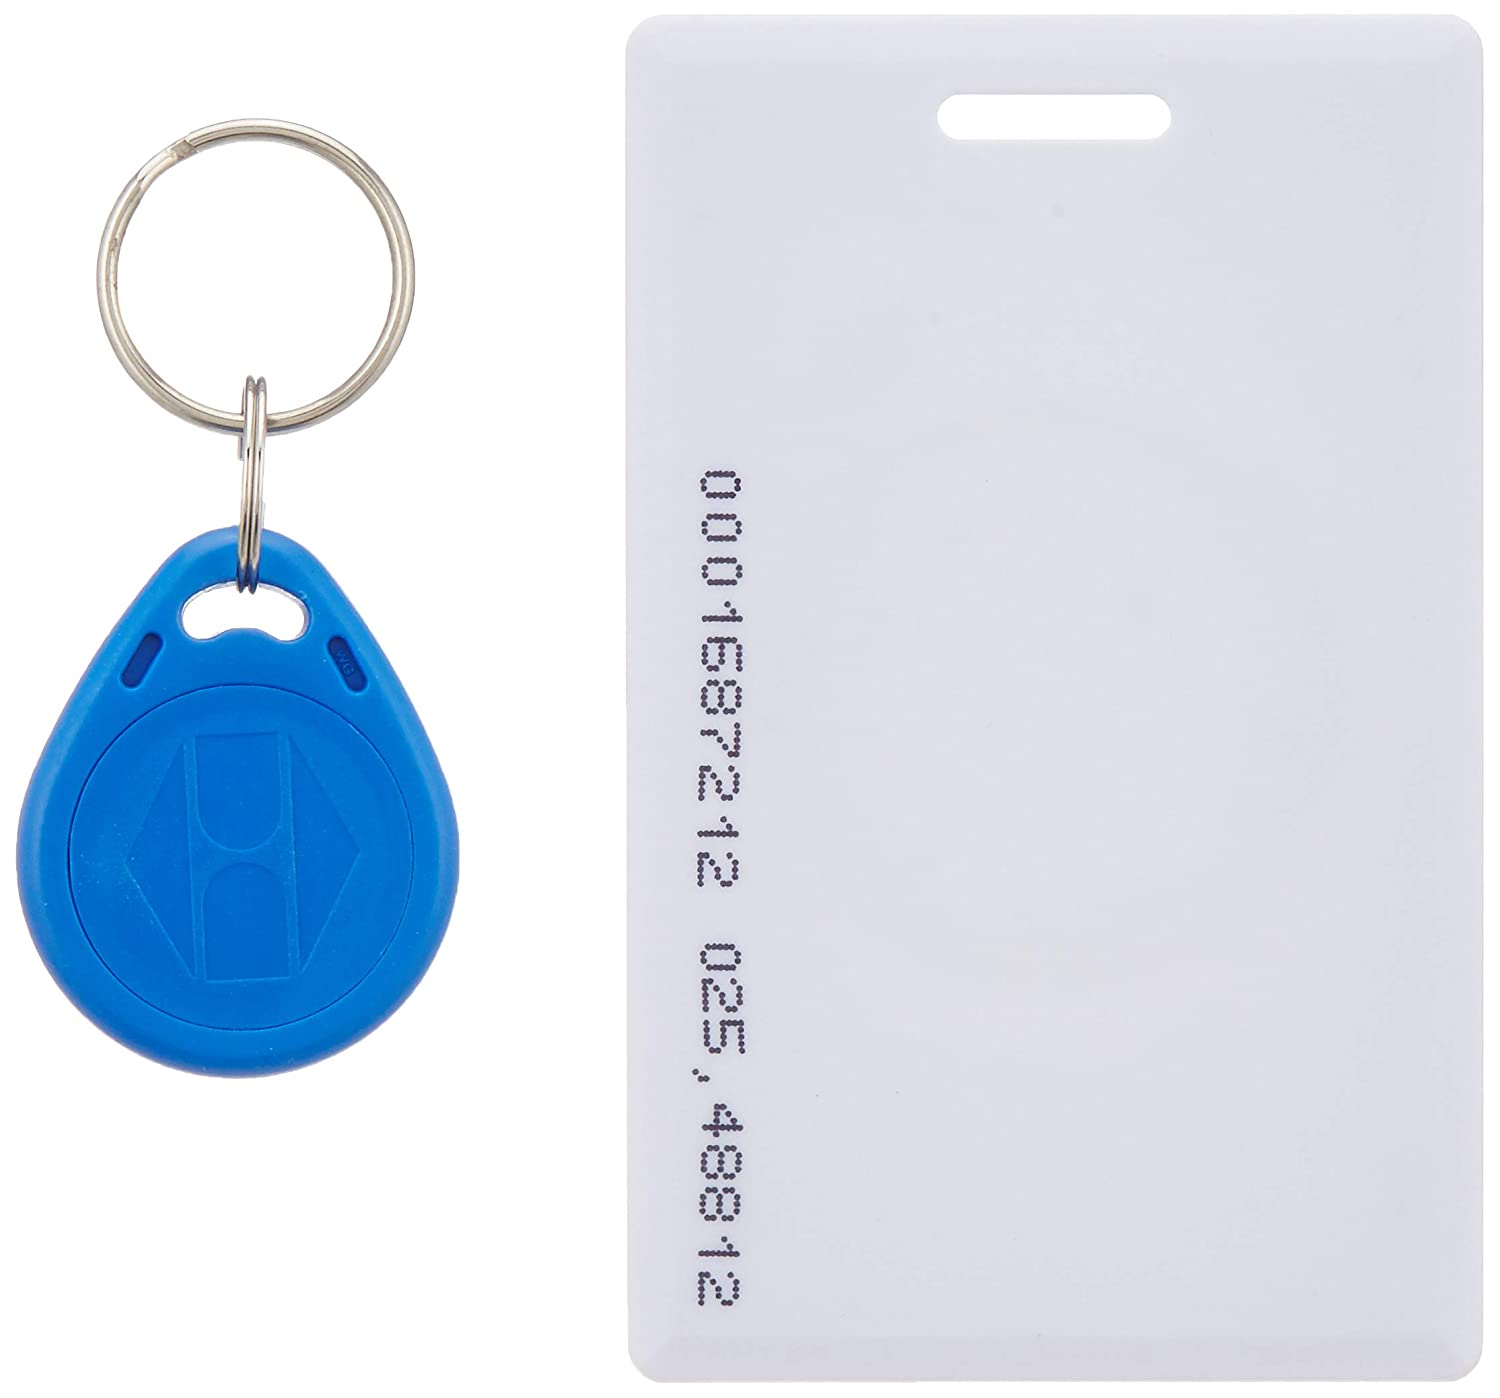
\includegraphics[width=0.85\textwidth, center]{images/rfidTag.jpg}
        \caption{RFID Tag}
        \label{fig:rfidTag}
    \end{afigure}

    Pada RFID tag terdapat 2 jenis yaitu \textit{Read-Write} dan \textit{Only Read}. Selain itu RFID tag mempunyai 2 komponen utama yang penting, antara lain:

    \begin{itemize}[topsep=0pt,itemsep=0pt,partopsep=0pt, parsep=0pt,]
        \item IC (\textit{Integrated Circuit}) : berfungsi sebagai pemproses informasi, modulasi serta demodulasi sinyal RF, yang beroperasi dengan catudaya DC.
        \item ANTENNA : mempunyai fungsi untuk mengirim maupun menerima sinyal RF.
    \end{itemize}

    \item RFID \textit{Reader}
    
    Berfungsi untuk membaca data dari RFID Tag. RFID \textit{Reader} dibedakan menjadi 2 macam, antara lain :
    \begin{itemize}[topsep=0pt,itemsep=0pt,partopsep=0pt, parsep=0pt,]
        \item Pasif : hanya bisa membaca data dari RFID tag aktif
        \item Aktif : dapat membaca data RFID tag pasif
    \end{itemize}
\end{enumerate}

\subsection{HC-SR04}
Sensor ultrasonik adalah sebuah sensor yang mengubah besaran fisis berupa bunyi menjadi besaran listrik dan sebaliknya. Cara kerja sensor ini didasarkan pada prinsip dari pantulan suatu gelombang suara sehingga dapat dipakai untuk menafsirkan jarak suatu benda dengan frekuensi tertentu. Disebut sebagai sensor ultrasonik karena sensor ini menggunakan gelombang ultrasonik (bunyi ultrasonik). Bunyi ultrasonik bisa merambat melalui zat padat, cair dan gas. Reflektivitas bunyi ultrasonik di permukaan zat padat hampir sama dengan reflektivitas bunyi ultrasonik di permukaan zat cair. Akan tetapi, gelombang bunyi ultrasonik akan diserap oleh tekstil dan busa.

\begin{afigure} 
    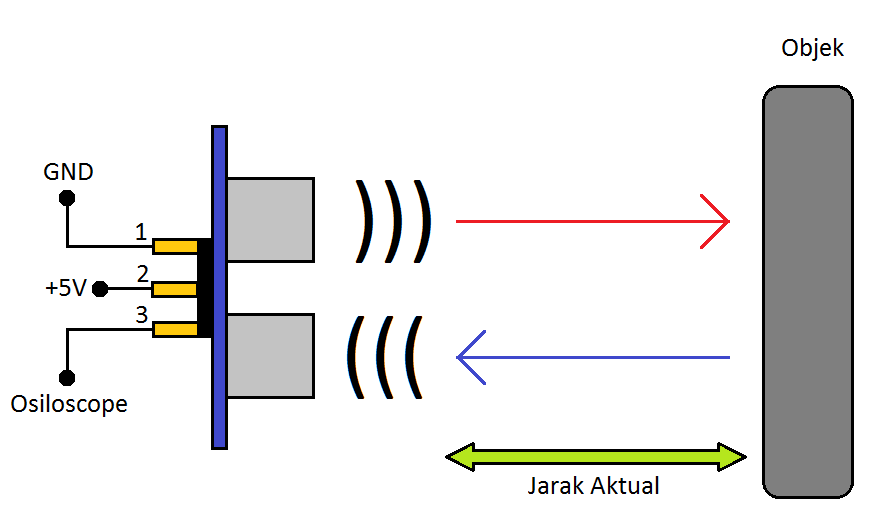
\includegraphics[width=0.85\textwidth, center]{images/cara kerja ultrasonik.png}
    \caption{Cara Kerja Sensor Ultrasonik}
    \label{fig:caraKerjaUltrasonic}
\end{afigure}

Secara umum, alat ini akan menembakkan gelombang ultrasonik menuju suatu area atau suatu target. Setelah gelombang menyentuh permukaan target, maka target akan memantulkan kembali gelombang tersebut. Gelombang pantulan dari target akan ditangkap oleh sensor, kemudian sensor menghitung selisih antara waktu pengiriman gelombang dan waktu gelombang pantul diterima \thecite{limantara2017a}. Ilustrasinya bisa dilihat pada gambar ~\ref{fig:caraKerjaUltrasonic}.

\begin{figure} [H]
    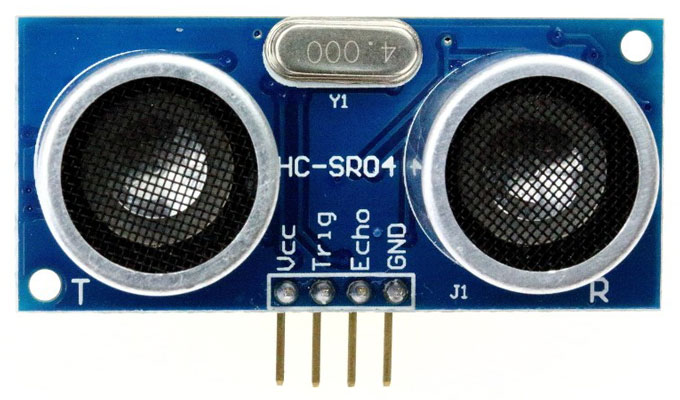
\includegraphics[width=0.85\textwidth, center]{images/ultrasonik.jpg}
    \caption{Sensor Ultrasonik}
    \label{fig:SensorUltrasonicHC-SR04}
\end{figure}

HC-SR04 merupakan sensor ultrasonik yang berfungsi sebagai pengirim, penerima, dan pengontrol gelombang ultrasonik. Alat ini bisa digunakan untuk mengukur jarak benda dari 2cm-4m dengan akurasi 3mm. Alat ini memiliki 4 pin, pin Vcc, Gnd, Trigger, dan Echo. Pin Vcc untuk listrik positif dan Gnd untuk ground-nya. Pin Trigger untuk trigger keluarnya sinyal dari sensor dan pin Echo untuk menangkap sinyal pantul dari benda. Sensor ultrasonik HC-SR04 bisa dilihat pada gambar ~\ref{fig:SensorUltrasonicHC-SR04}.

\subsection{SG90}
SG90 adalah sebuah servo kecil dengan output power yang tinggi. Motor ini dapat berotasi sekitar 180 derajat dan bisa bekerja seperti servo lainnya hanya saja ukurannya lebih kecil \thecite{wicaksono2018a}.

\begin{figure} [H]
    % 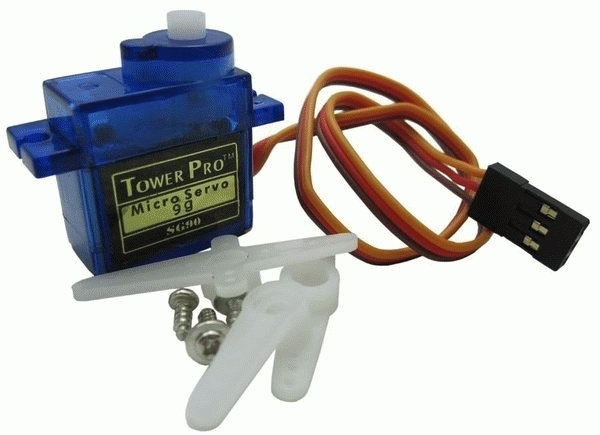
\includegraphics[width=0.85\textwidth, center]{images/servo.jpg}
    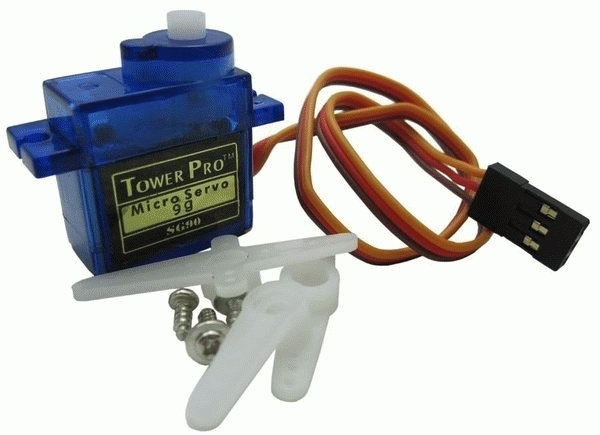
\includegraphics[width=0.50\textwidth, center]{images/servo.jpg}
    \caption{Servo SG90}
    \label{fig:servo}
\end{figure}

Gambar ~\ref{fig:servo} merupakan gambar dari servo SG90.

\subsection{Push Button}
Push Button atau yang juga disebut \textit{tactile switch} adalah sebuah tombol yang apabila ditekan posisinya akan kembali pada saat dilepaskan. Push button berbeda dengan saklar yang posisinya akan tetap atau terkunci sampai ditekan kembali. Push button memiliki 4 buah kaki, dua berada di sisi kiri, dan dua kaki lainnya berada di sebelah kanan yang saling tidak terhubung. Pada saat tombol ditekan, maka kedua kaki tersebut akan tersambung untuk mengalirkan arus listrik ke sisi lain \thecite{dinarta2018a}. gambar ~\ref{fig:pushbutton} merupakan gambar dari push button.

\begin{figure} [H]
    % 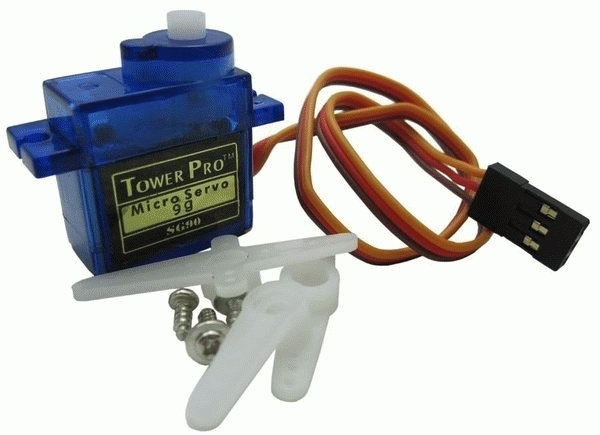
\includegraphics[width=0.85\textwidth, center]{images/servo.jpg}
    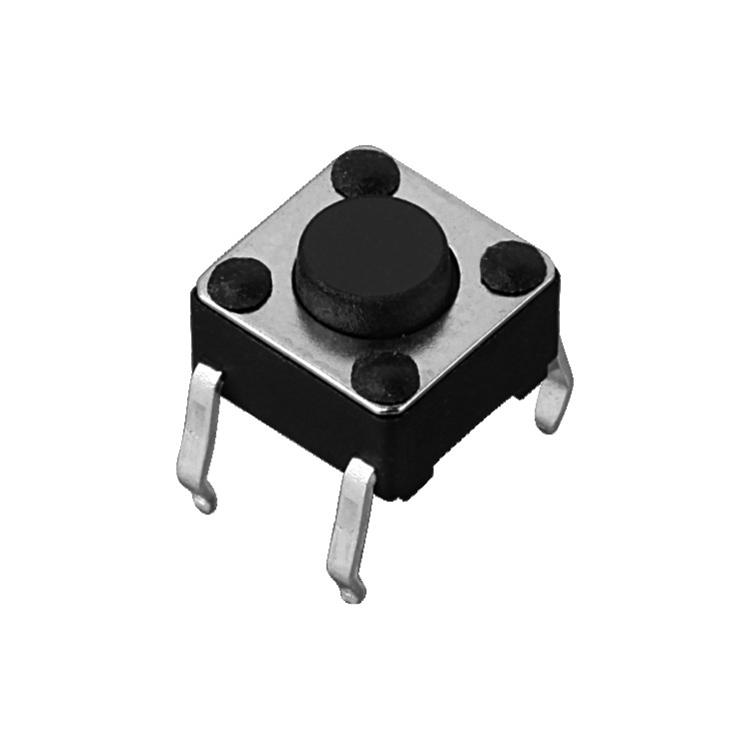
\includegraphics[width=0.50\textwidth, center]{images/pushbutton.jpg}
    \caption{Push Button}
    \label{fig:pushbutton}
\end{figure}

\subsection{Kamera Raspberry Pi v2}
Modul Kamera v2 memiliki sensor Sony IMX219 8-megapiksel. Modul Kamera dapat digunakan untuk mengambil video definisi tinggi, dan juga foto. Gambar ~\ref{fig:raspicamera} merupakan gambar dari kamera Raspberry Pi.

\begin{afigure} 
    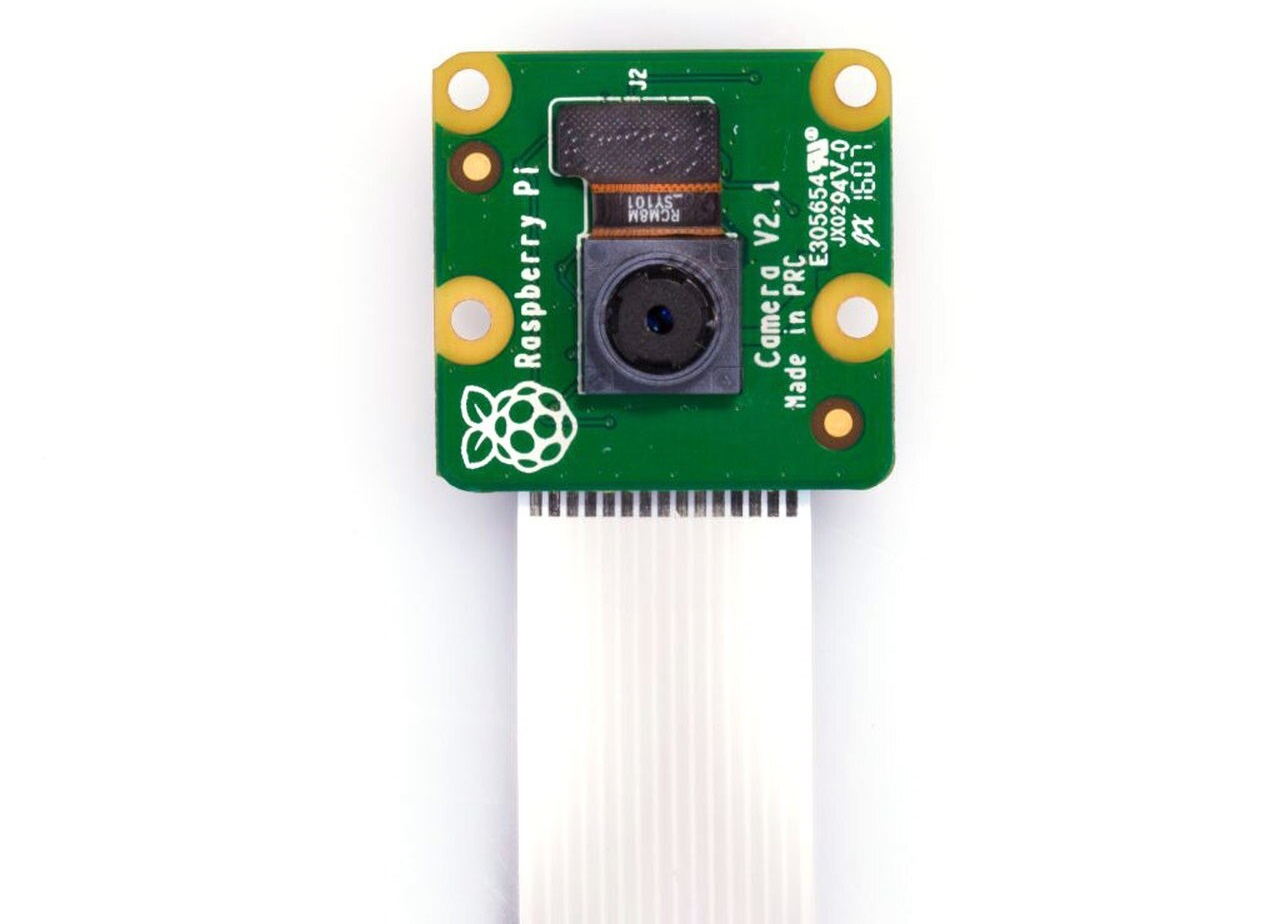
\includegraphics[width=0.85\textwidth, center]{images/raspicamera.jpg}
    \caption{ Kamera Raspberry Pi}
    \label{fig:raspicamera}
\end{afigure}

% \subsection{API, REST API, dan RESTful API}


    \chapter{METODE PENELITIAN}

\setlength{\intextsep}{0cm}
% \setlength{\textfloatsep}{-1cm}

\section{Waktu dan Lokasi Penelitian}
Penelitian ini dilaksanakan dari bulan juli 2020 sampai dengan bulan november 2020. Lokasi penelitian dilakukan di Laboratorium Rekayasa Perangkat Lunak Fakultas Matematika dan Ilmu Pengetahuan Alam, Universitas Hasanuddin.

\section{Tahapan Penelitian}

\begin{table} [H]
    \begin{tabular}{|>{\centering\arraybackslash}m{1\linewidth} |}
        \hline
        \textbf{Analisis Kebutuhan}\\ 
        Pada tahapan ini merupakan tahap awal yaitu menganalisis semua kebutuhan yang diperlukan selama meneliti seperti pengumpulan teori terkait dengan penelitian yang terdapat dalam buku atau jurnal.\\
        \hline
    \end{tabular}
\end{table}

\begin{center}
    \bigg\downarrow
\end{center}

\begin{table} [H]
    \begin{tabular}{|>{\centering\arraybackslash}m{1\linewidth} |}
        \hline
        \textbf{Desain Sistem}\\ 
        Pada tahap ini dilakukan perancangan sistem yang akan dibangun seperti, rancangan sistem, rancangan skematik alat, \textit{use case} diagram, \textit{activity} diagram dan perancangan aplikasi web.\\
        \hline
    \end{tabular}
\end{table}

\begin{center}
    \bigg\downarrow
\end{center}

\begin{table} [H]
    \begin{tabular}{|>{\centering\arraybackslash}m{1\linewidth} |}
        \hline
        \textbf{Implementasi}\\ 
        Pada tahapan ini dilakukan implementasi dari hasil perancangan pada tahapan sebelumnya. Di tahapan inilah pembangunan sistem parkir, perangkaian sensor-sensor dan \textit{microcontoller} dilakukan.\\
        \hline
    \end{tabular}
\end{table}

\begin{center}
    \bigg\downarrow
\end{center}

\begin{table} [H]
    \begin{tabular}{|>{\centering\arraybackslash}m{1\linewidth} |}
        \hline
        \textbf{Pengujian Sistem}\\ 
        Pada tahapan ini hasil dari pembuatan sistem siap untuk diimplementasikan. Sensor ditempatkan di tempat yang sudah disediakan, maka alat ini akan mengumpulkan data yang dibutuhkan seperti nomor plat, id rfid, dan jarak ultrasonik. Data yang berhasil dikumpulkan akan disimpan di database dan bisa dilihat di web.\\
        \hline
    \end{tabular}
\end{table}

\begin{center}
    \bigg\downarrow
\end{center}

\begin{table} [H]
    \begin{tabular}{|>{\centering\arraybackslash}m{1\linewidth} |}
        \hline
        \textbf{Kesimpulan}\\ 
        Pada tahap ini merupakan tahap penting terakhir dari penelitian ini. Pada tahapan ini hasil dari pembuatan sistem parkir sudah siap untuk diimplementasikan.\\
        \hline
    \end{tabular}
\end{table}

\section{Sumber Data}
Sumber data dari penelitian ini menggunakan data primer yang didapatkan secara langsung dari sensor yang digunakan dalam sistem parkir.

\section{Rancangan Sistem}
Sensor dan kamera akan terhubung dengan raspberry pi. Berikut ini adalah gambaran mengenai rancangan dari penelitian ini :\newline

\begin{afigure} 
    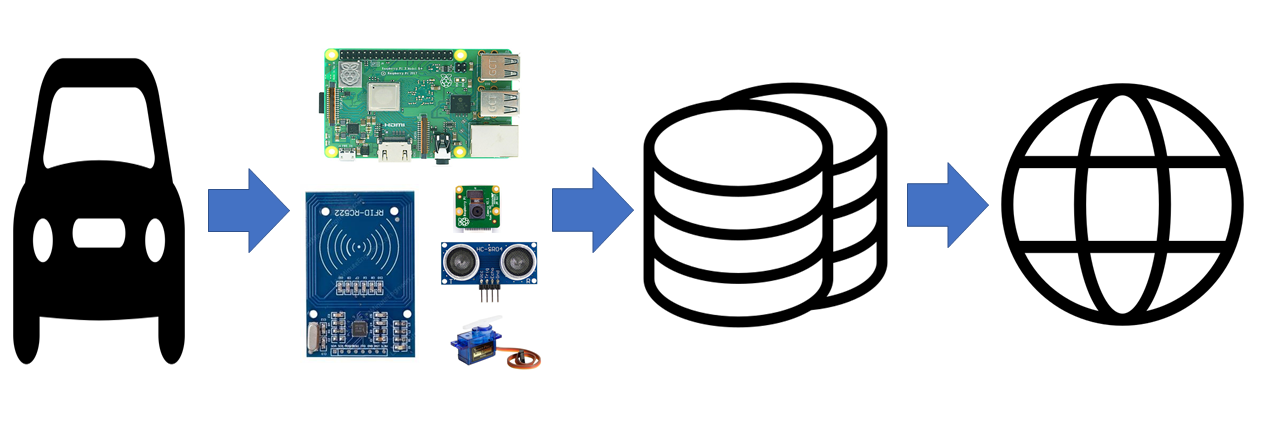
\includegraphics[width=0.85\textwidth, center]{images/rancangan sistem.png}
    \caption{Rancangan Sistem}
    \label{fig:RancanganSistem}
\end{afigure}

Pada gambar ~\ref{fig:RancanganSistem} saat pengemudi kendaraan menempelkan tag RFID mereka ke RFID reader, kamera pada raspberry akan mengambil gambar untuk di identifikasi nomor pelat tersebut. Hasil identifikasi akan berupa data nomor pelat kendaraan yang akan disimpan. Setelah itu servo yang berfungsi sebagai palang pintu akan terbuka. Data yang dikumpulkan oleh sensor berupa Id RFID dan nomor pelat kendaraan dapat dilihat melalui aplikasi web.

\section{Rancangan \textit{Use Case} Diagram}
Rancangan \textit{use case} diagram pada penelitian ini dapat di gambarkan seperti diagram dibawah ini:

\begin{afigure} 
    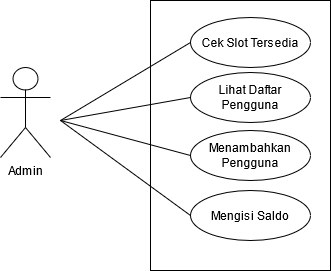
\includegraphics[width=0.85\textwidth, center]{images/Use Case Diagram revisi.png}
    \caption{Use Case Diagram}
    \label{fig:usecasediagram}
\end{afigure}

sesuai dengan gambar ~\ref{fig:usecasediagram}, sistem yang akan dibangun hanya terdapat satu jenis akun yaitu akun admin yang akan mengawasi seluruh aktivitas pemarkiran melalui aplikasi web sebagai \textit{user interface}.

\section{Instrumen Penelitian}
Instrumen penelitian pada penelitian ini meliputi kebutuhan perangkat keras dan kebutuhan perangkat lunak.

\begin{enumerate}[topsep=0pt,itemsep=0pt,partopsep=0pt, parsep=0pt]
\item Kebutuhan perangkat keras
    \begin{itemize}[topsep=0pt,itemsep=0pt,partopsep=0pt, parsep=0pt,]
        \item Raspberry Pi
        \item Sensor RFID MFRC522
        \item Sensor Ultrasonik HC-SR04
        \item Servo SG90
        \item Camera Raspberry Pi v2 8mp
        \item Push Button
        \item Kabel Jumper
        \item Bread Board
        \item Memori Card
    \end{itemize}
\item Kebutuhan perangkat lunak
    \begin{itemize}[topsep=0pt,itemsep=0pt,partopsep=0pt, parsep=0pt,]
        \item \textit{Operating System (OS)} Raspbian
        \item \textit{Python Programming Language} (bahasa pemrograman yang digunakan)
        \item Visual Studio Code
        \item Web Browser
    \end{itemize}
\end{enumerate}
    \chapter{HASIL DAN PEMBAHASAN}

\section{Hasil Rancangan Sistem Identifikasi Kendaraan Pada Pemarkiran Dengan Pengenalan Citra Dan Pembacaan RFID}

\subsection{Hasil Perancangan Perangkat Keras}
\begin{figure} [H]
    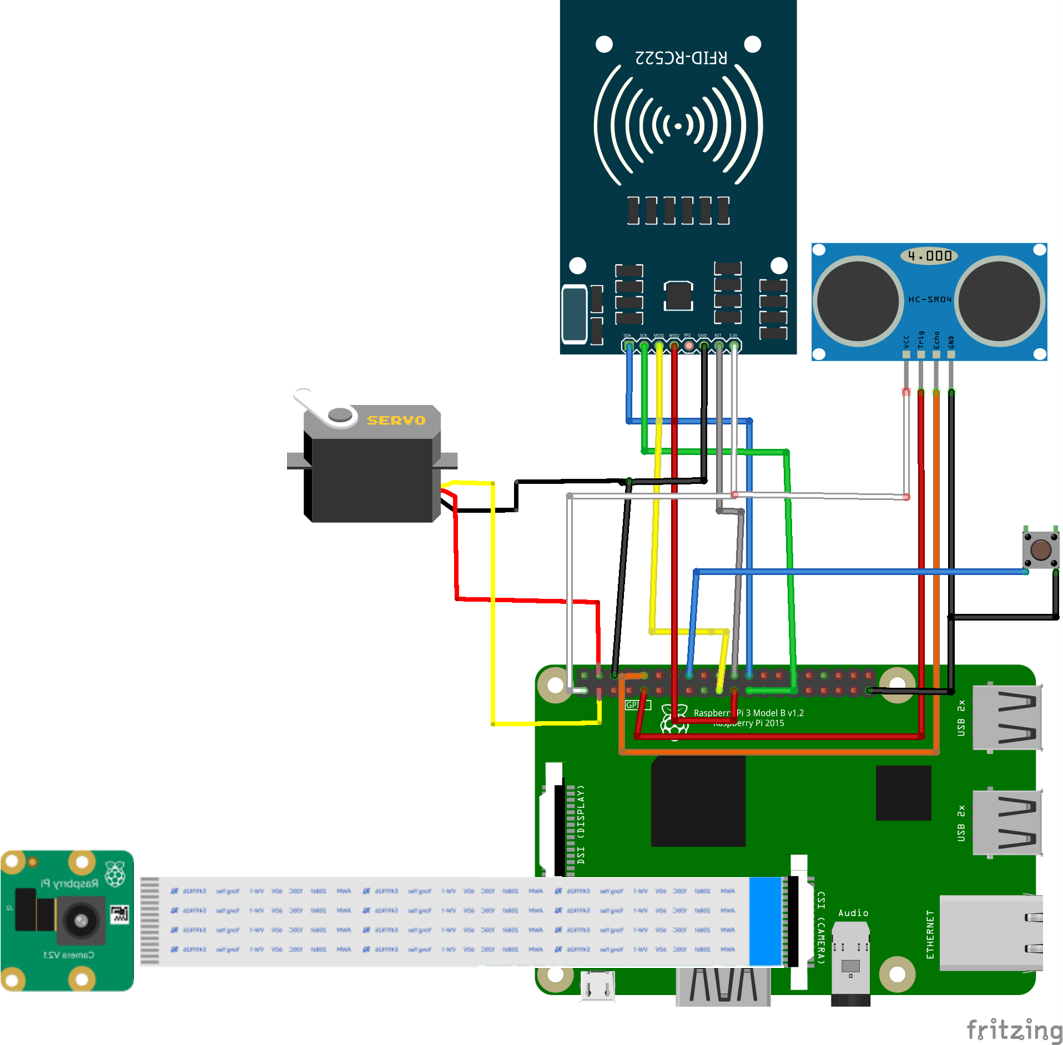
\includegraphics[width=0.85\textwidth, center]{images/skematik_full_dan_button_dan_kamera.png}
    \caption{Rangkaian Skematik Alat}
    \label{fig:rangkaianSkematikAlat}
\end{figure}

\begin{figure} [H]
    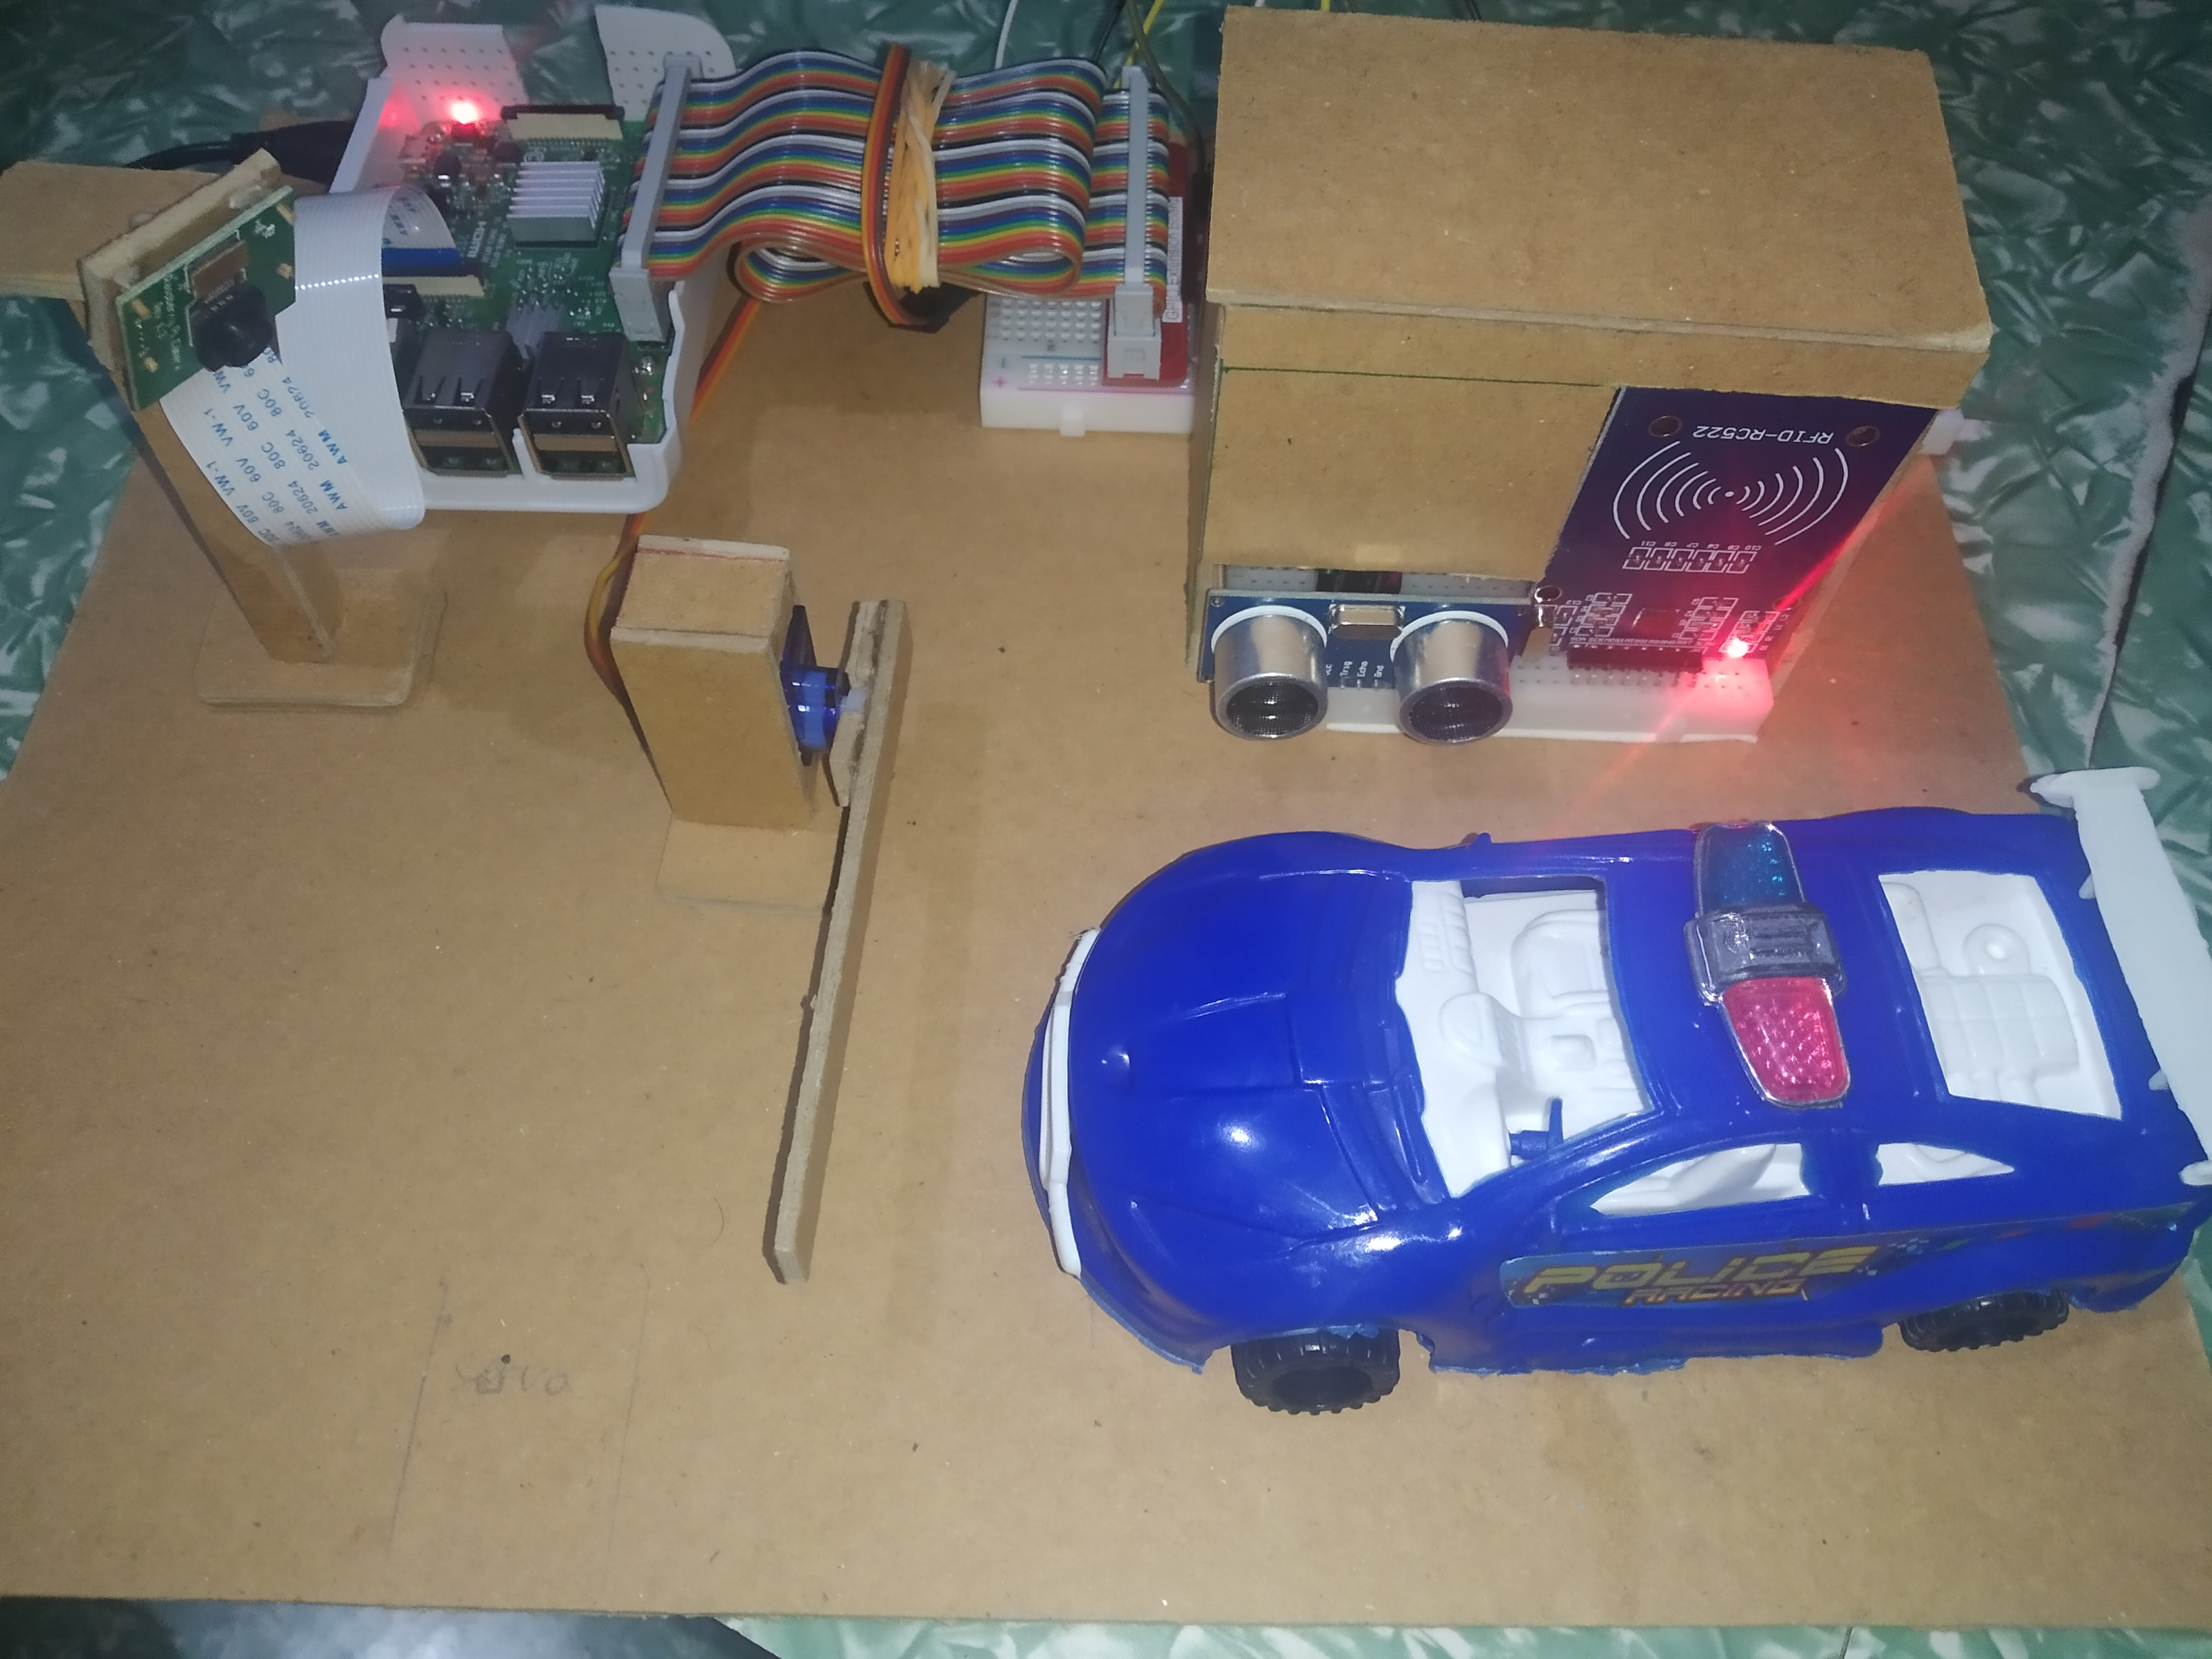
\includegraphics[height=9cm, width=0.85\textwidth, center]{images/alat-full-mobil.jpg}
    \caption{Hasil Rancangan dan Pemasangan Alat}
    \label{fig:alatfullmobil}
\end{figure}

\begin{figure} [H]
    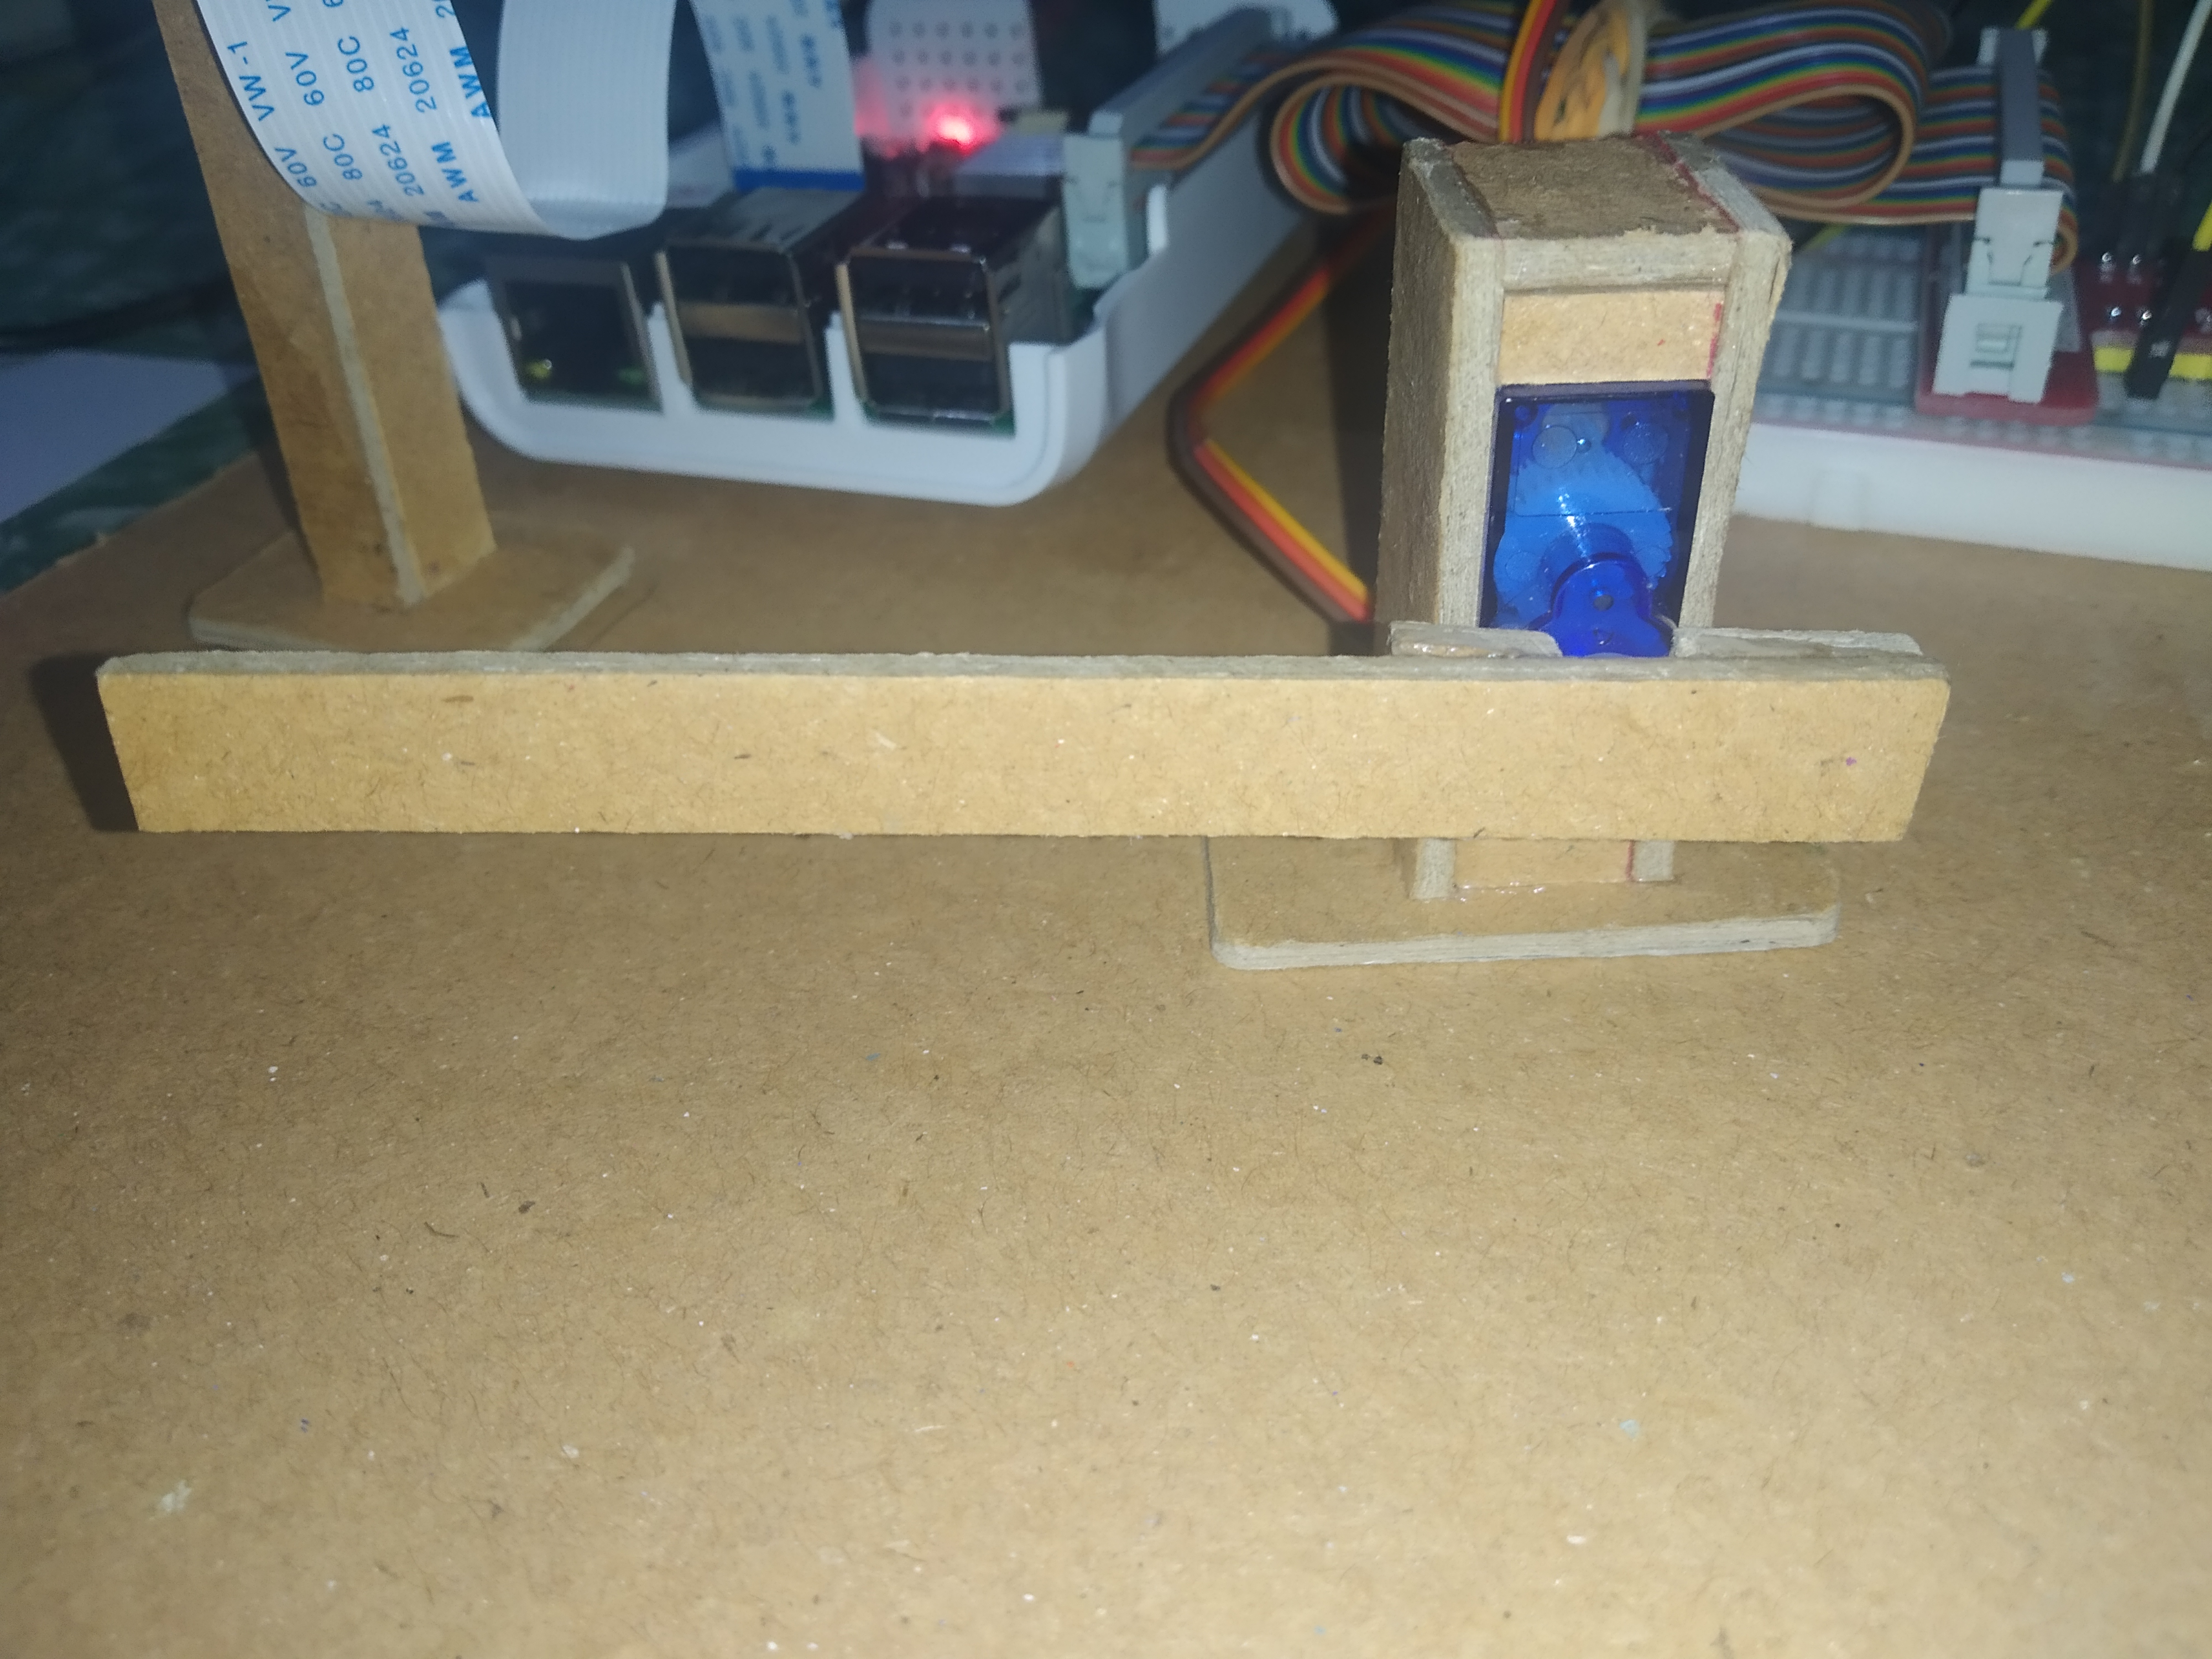
\includegraphics[height=7cm, width=0.5\textwidth, center]{images/alat-servo.jpg}
    \caption{Hasil Rancangan Servo}
    \label{fig:alatservo}
\end{figure}

\begin{figure} [H]
    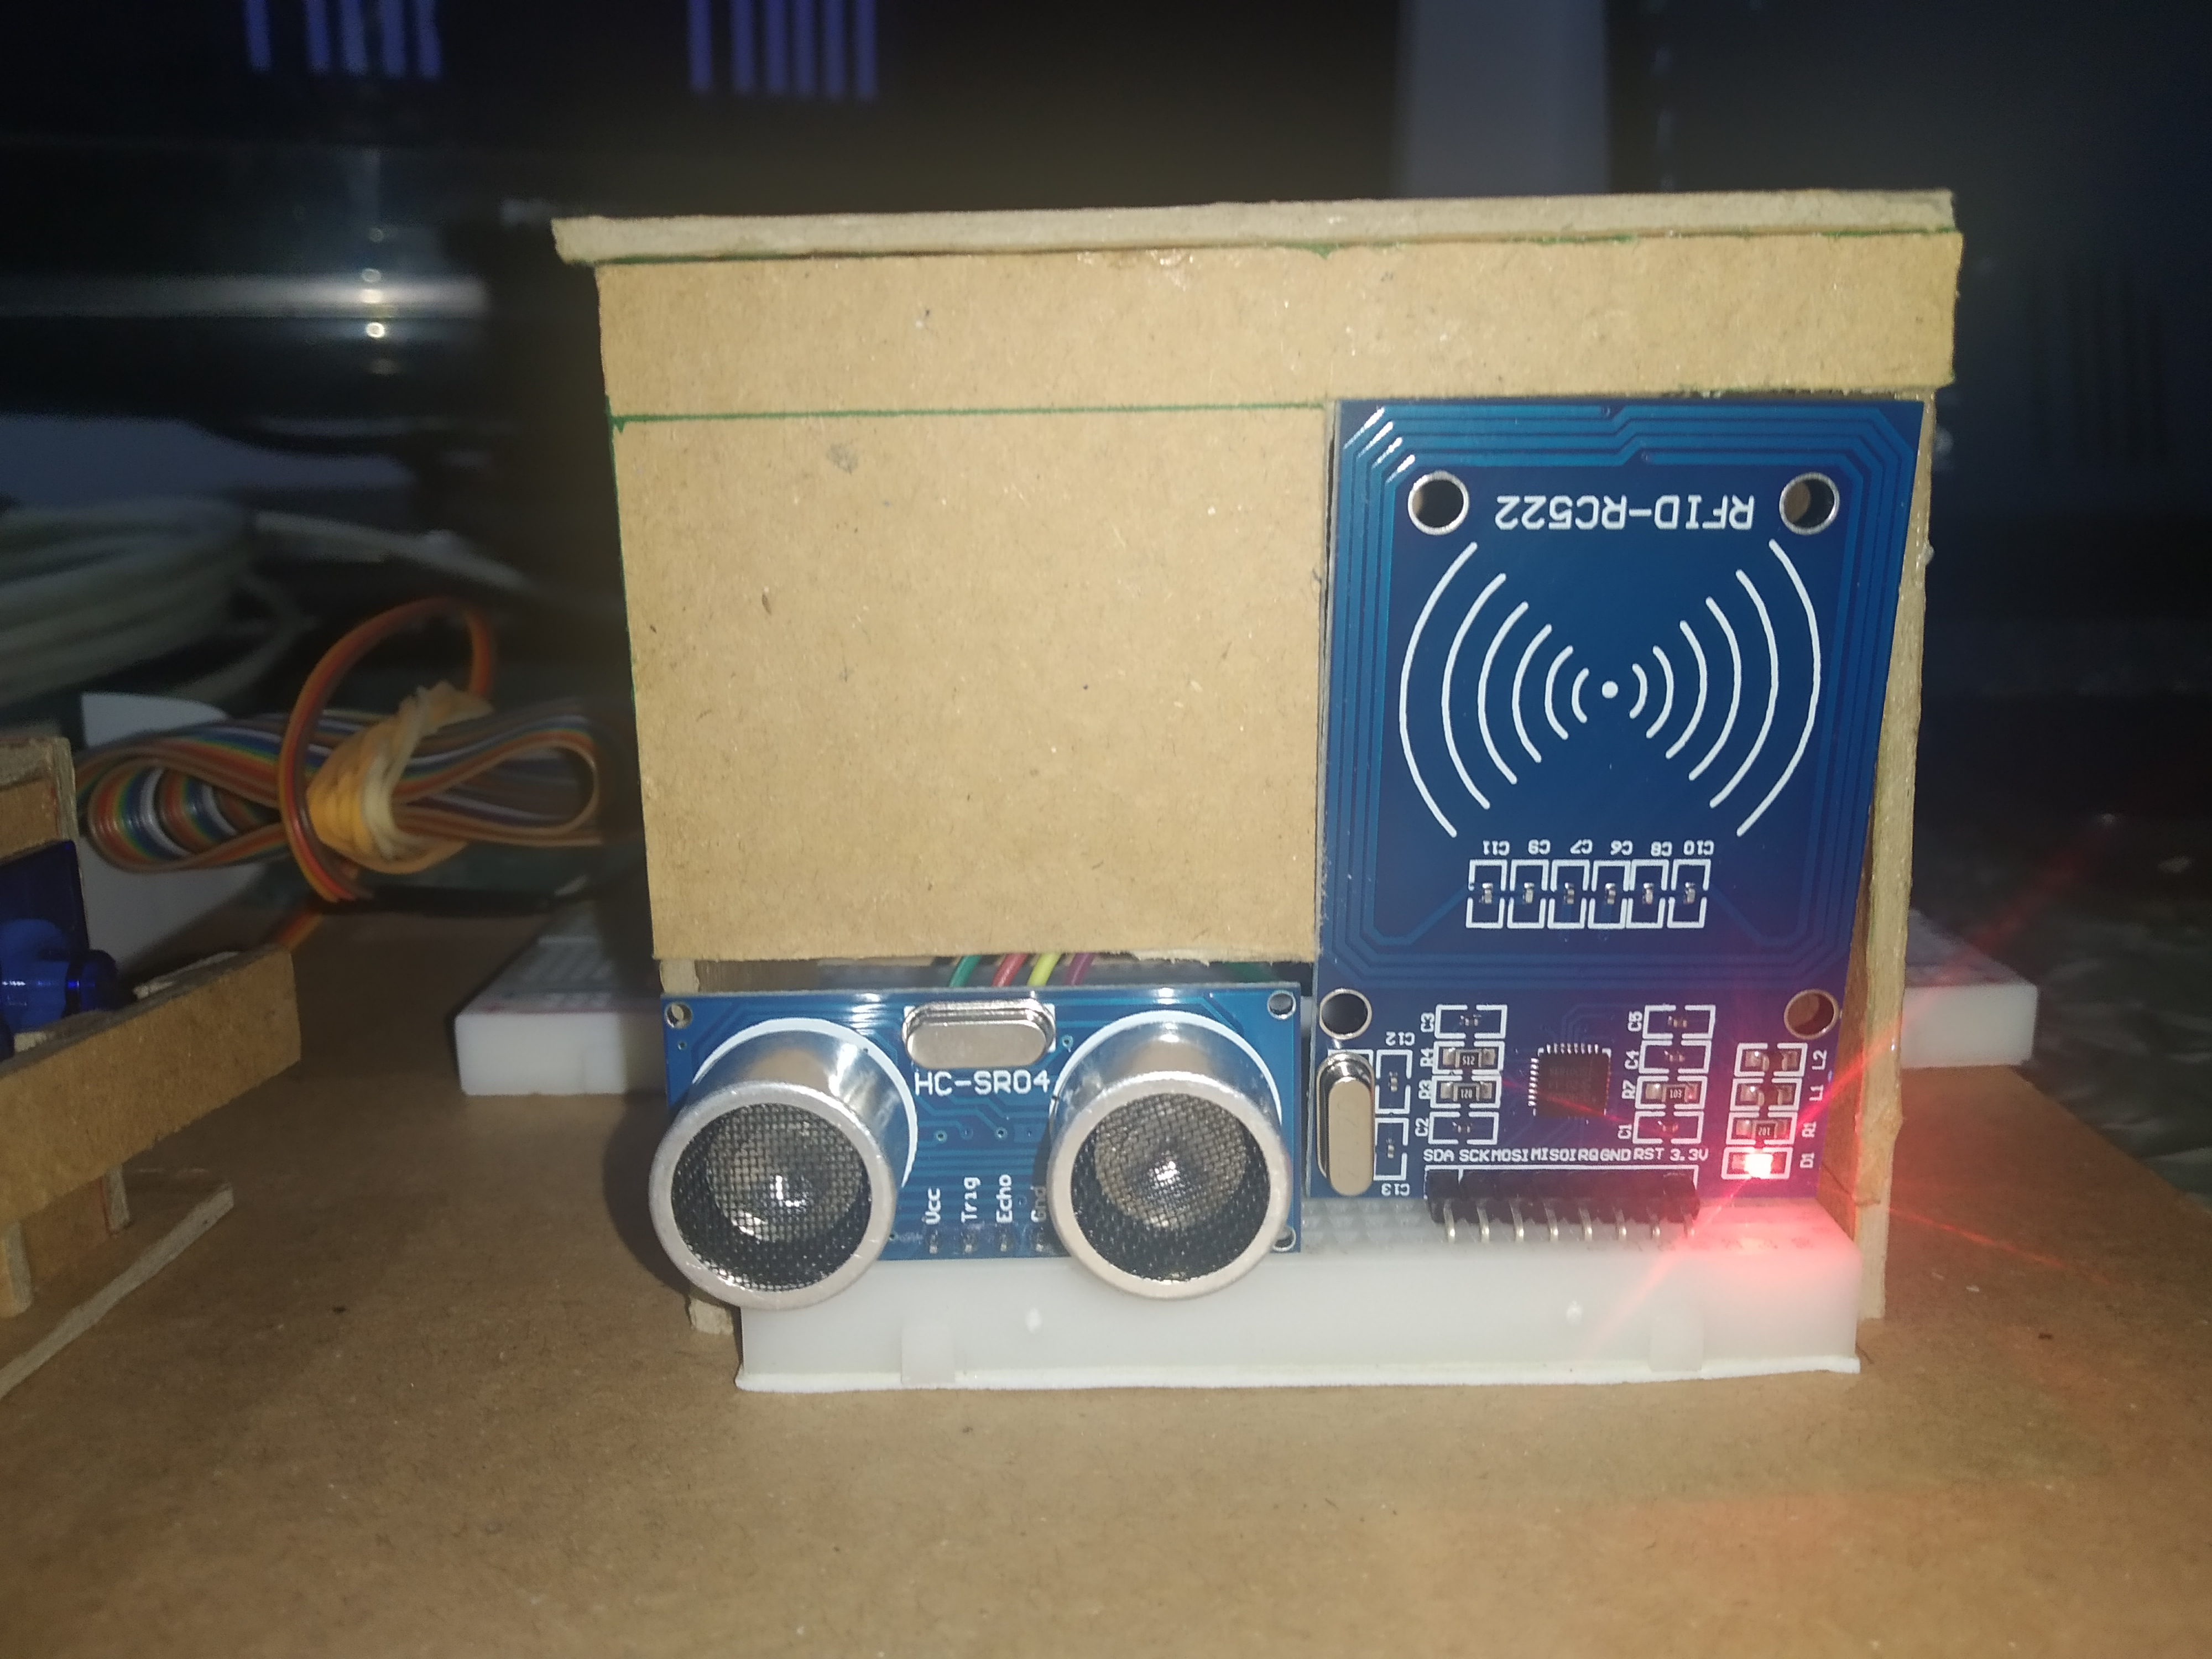
\includegraphics[height=7cm, width=0.65\textwidth, center]{images/alat-ultra&rfid.jpg}
    \caption{Hasil Rancangan Ultrasonik dan RFID}
    \label{fig:alatultrarfid}
\end{figure}

\begin{figure} [H]
    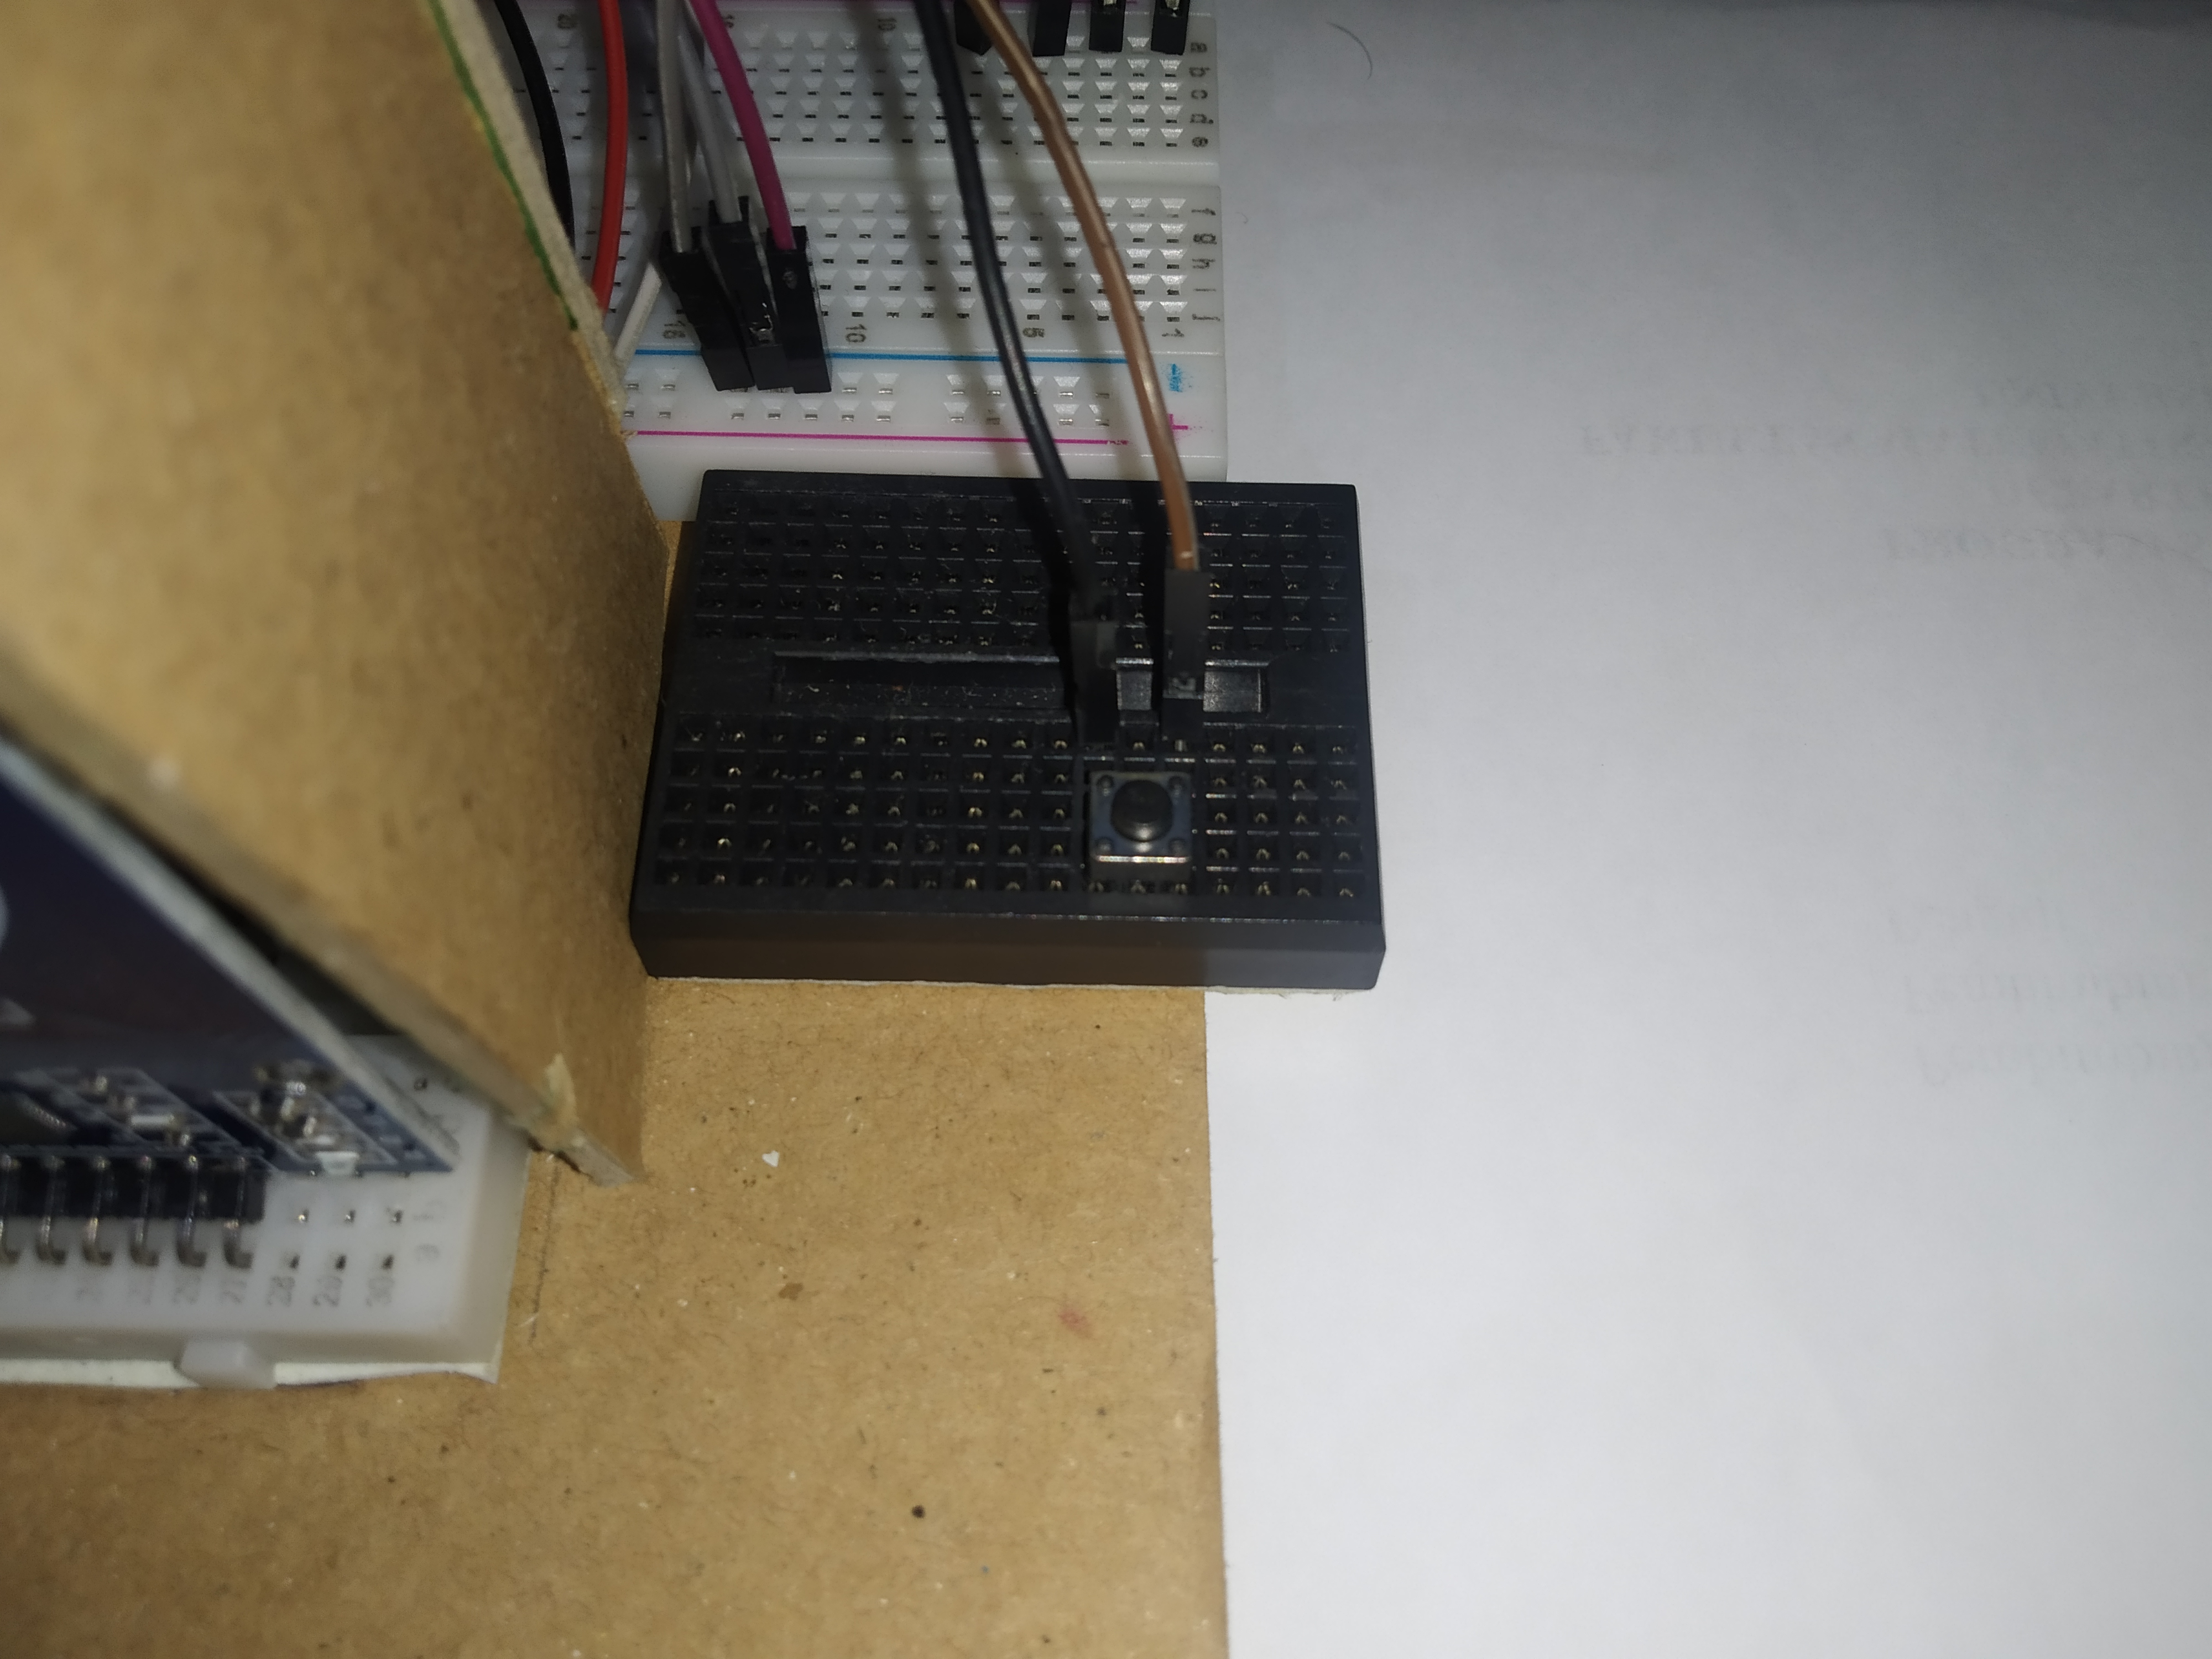
\includegraphics[height=7cm, width=0.65\textwidth, center]{images/alat-button.jpg}
    \caption{Hasil Rancangan Button}
    \label{fig:alatbutton}
\end{figure}

\begin{figure} [H]
    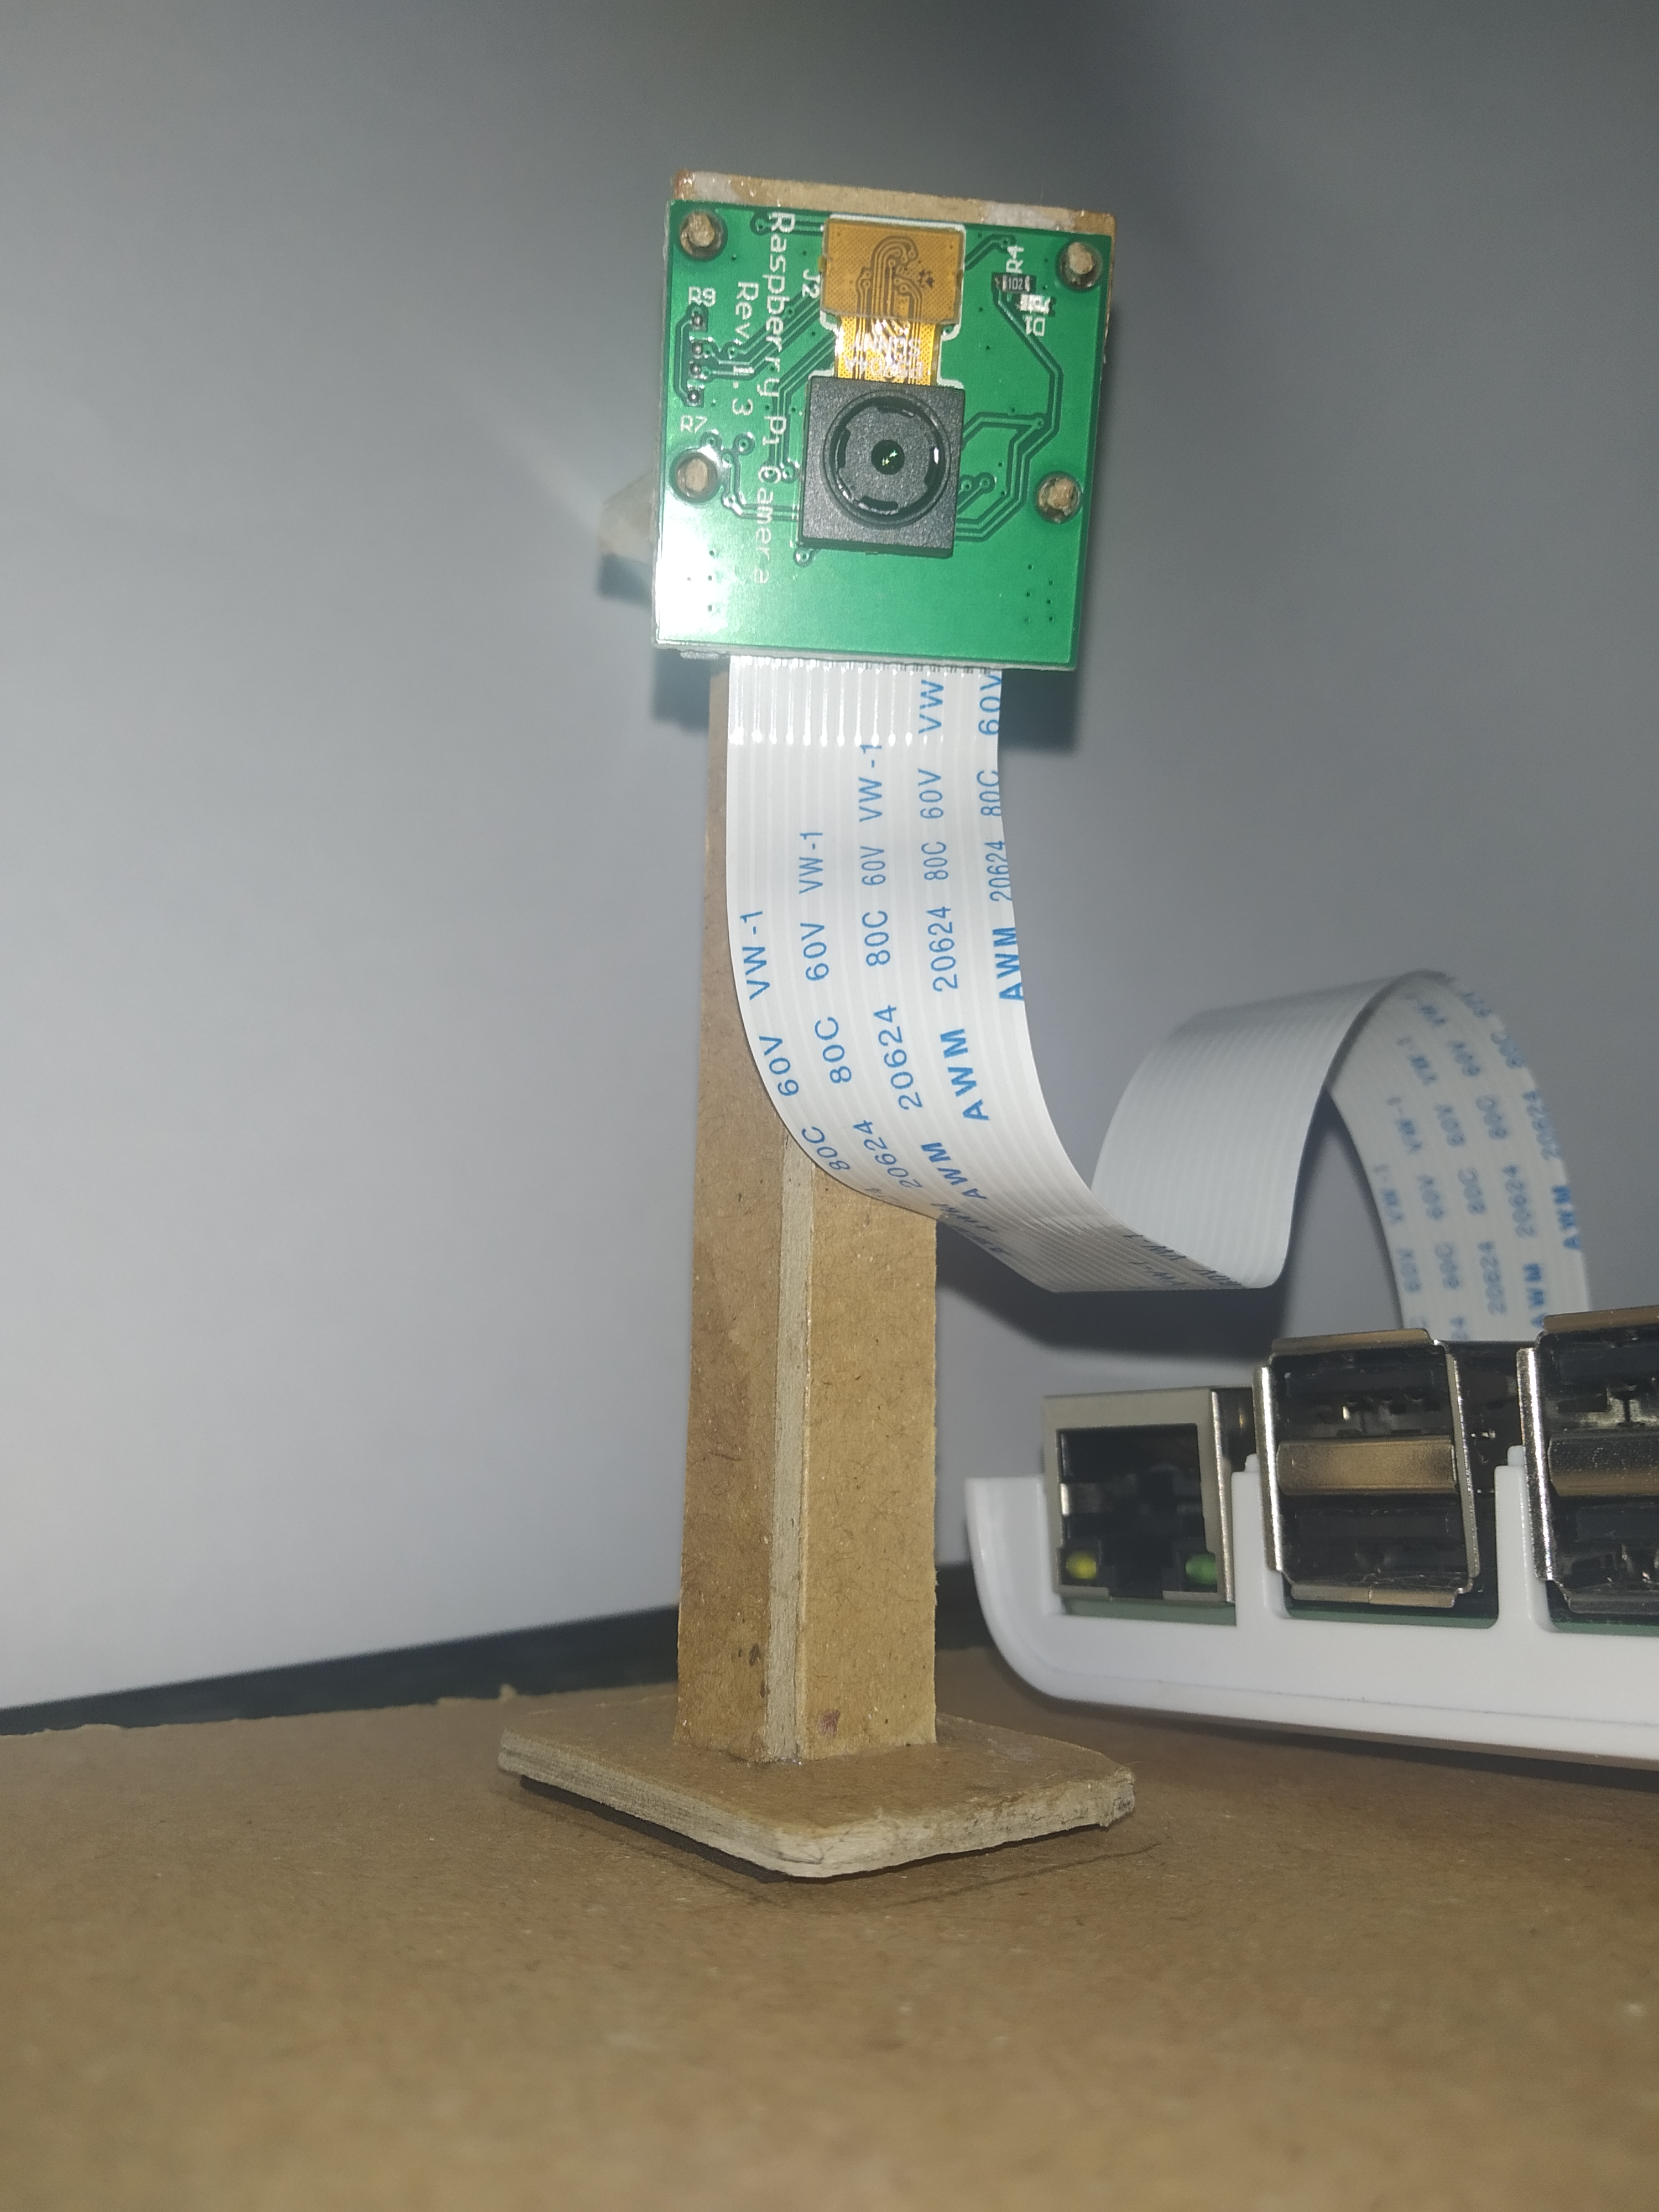
\includegraphics[height=7cm, width=0.5\textwidth, center]{images/alat-kamera.jpg}
    \caption{Hasil Rancangan Kamera}
    \label{fig:alatkamera}
\end{figure}

Pada gambar diatas merupakan rangkaian perangkat keras untuk penelitian di mana seluruh perangkat dirangkai menjadi satu rangkaian.  Gambar ~\ref{fig:alatfullmobil} merupakan hasil dari rancangan dari penelitian yang dilakukan, yang dimana masih bersifat \textit{prototype}. Pada gambar ~\ref{fig:alatservo} dapat dilihat bahwa servo digambarkan sebagai palang parkir. Pada gambar ~\ref{fig:alatultrarfid} dapat dilihat sensor ultrasonik yang akan membaca jarak dari kendaraan untuk menentukan apakah kendaraan masih ada atau sudah tidak ada dan sensor rfid untuk membaca kartu atau tag dari pengendara. Pada gambar ~\ref{fig:alatkamera} dapat dilihat kamera raspberry yang digunakan untuk mengambil nomor plat kendaraan. \textit{Activity} diagram pada sistem yang dibuat bisa dilihat pada gambar ~\ref{fig:diagrammasuk} dan gambar ~\ref{fig:diagramkeluar}.\newline

\begin{figure} [H]
    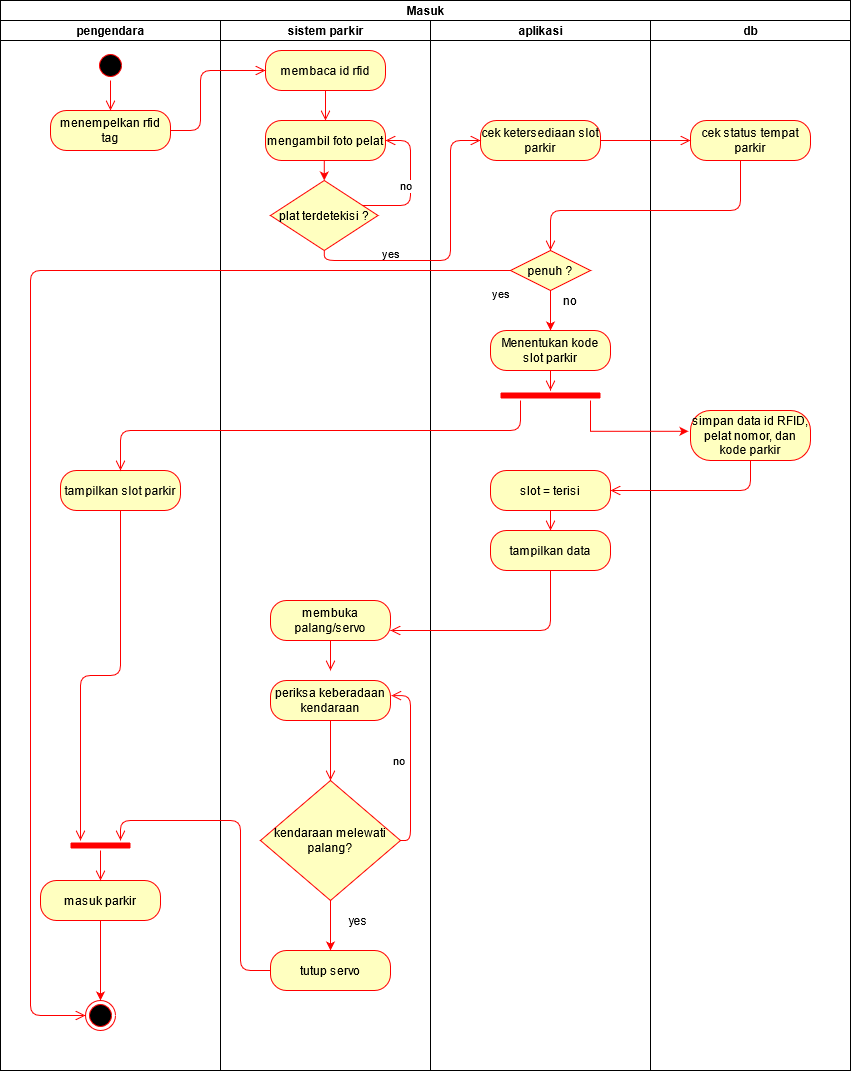
\includegraphics[width=1\textwidth, center]{images/activity diagram skripsi masuk.png}
    \caption{Activity Diagram Masuk}
    \label{fig:diagrammasuk}
\end{figure}

\begin{figure} [H]
    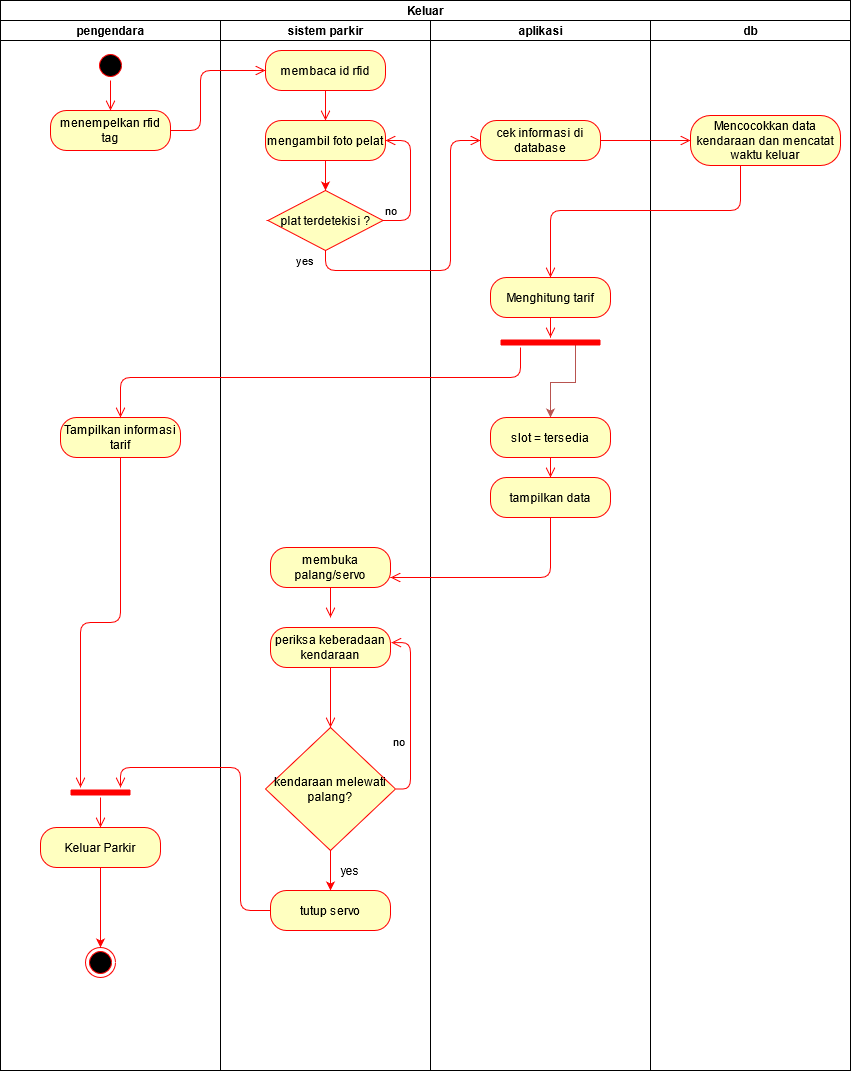
\includegraphics[width=1\textwidth, center]{images/activity diagram skripsi keluar.png}
    \caption{Activity Diagram Keluar}
    \label{fig:diagramkeluar}
\end{figure}

\subsection{Raspberry Pi dan RFID MFRC522}
\begin{figure} [H]
    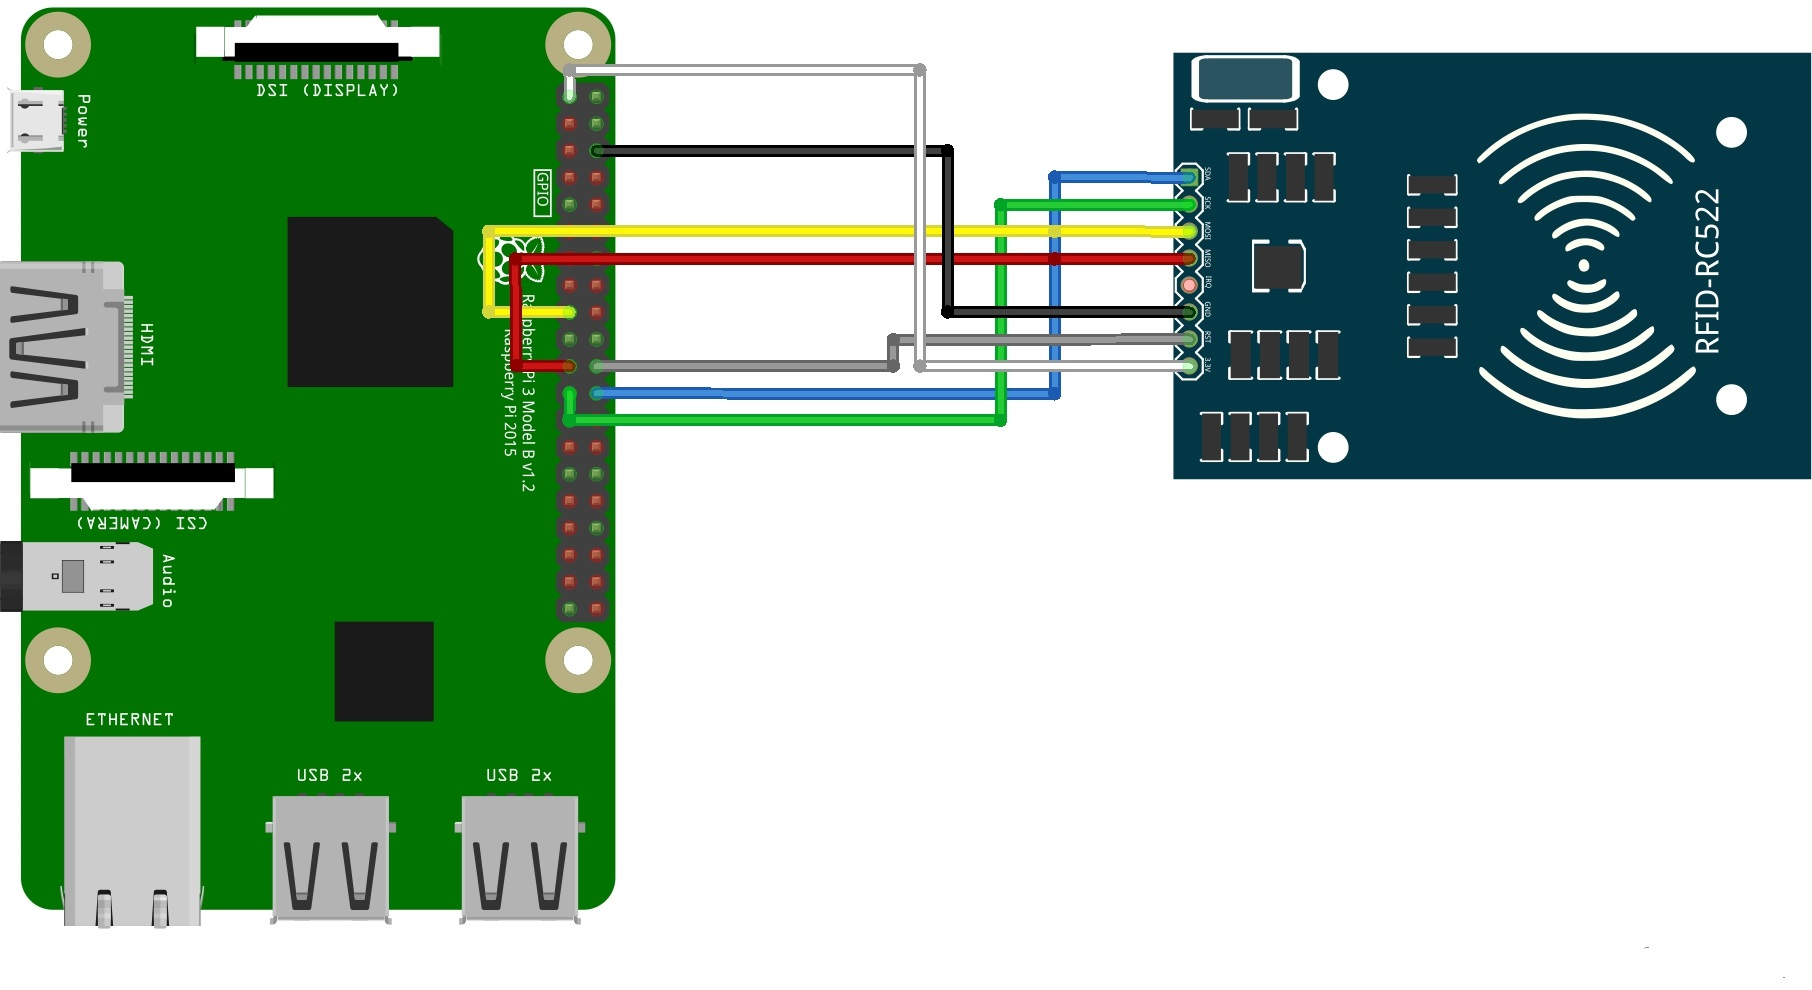
\includegraphics[width=0.85\textwidth, center]{images/skematik_rfid.jpg}
    \caption{Ragkaian Raspberry Pi dan RFID}
    \label{fig:skematikRfid}
\end{figure}

Berdasarkan gambar ~\ref{fig:skematikRfid} Menunjukkan Raspberry Pi sebagai mikrokontroler untuk menghubungkan sensor RFID yang akan membaca kartu atau tag dari pengendara. Untuk pin pada Raspberry Pi dihubungkan pada sensor RFID dapat dilihat pada tabel ~\ref{table:tableRfid}.\newline

\begin{atable}
    \caption{Rangkaian pin RFID ke Raspberry Pi}
    \label{table:tableRfid}
    \csvreader[
        % column count = 11,
        respect underscore=true,
        tabular=cc,
        head to column names,
        before table=\rowcolors{2}{gray!15}{gray!30},
        table head= \rowcolor{gray!50!black} 
            \color{white} RFID & 
            \color{white} RASPBERRY PI 
            \\]
        {tables/tablerfid.csv}
        {
            RFID=\RFID, 
            RASPBERRYPI=\RASPBERRYPI}
        {
            \RFID & 
            \RASPBERRYPI}
\end{atable}

Berikut ini dilakukan pengujian jarak baca kartu RFID yang berfungsi untuk melihat jarak maksimum keterbacaan RFID dari bagian pembaca ke kartu RFID. Pengujian ini dilakukan dengan cara meletakkan kartu RFID dengan memberi jarak tertentu pada area pembacaan. Hasil pengujian dapat dilihat pada tabel ~\ref{table:tableUjiRfid}.

\begin{table}[H]
    \caption{Hasil uji jarak baca RFID}
    \label{table:tableUjiRfid}
    \centering
    \csvreader[
        % column count = 11,
        respect underscore=true,
        tabular=ccc,
        head to column names,
        before table=\rowcolors{2}{gray!15}{gray!30},
        table head= \rowcolor{gray!50!black} 
            \color{white} No. & 
            \color{white} Jarak (mm) & 
            \color{white} Terbaca
            \\]
        {tables/hasil-uji-jarak-rfid.csv}
        {
            No=\No, 
            Jarak=\Jarak,
            Terbaca=\Terbaca}
        {
            \No & 
            \Jarak &
            \Terbaca}
\end{table}

Berdasarkan data hasil pengujian sensor RFID pada tabel ~\ref{table:tableUjiRfid}, pengambilan data dilakukan sebanyak dua puluh kali. Dari data hasil pengukuran yang pertama sampai ke lima belas dengan jarak 0 mm sampai 28 mm, kartu RFID dapat terbaca dengan baik dan pengukuran ke enam belas sampai dua puluh dengan jarak 30 mm sampai 38 mm, kartu sudah tidak bisa tebrbaca.

\subsection{Raspberry Pi dan HC-SR04}
\begin{figure} [H]
    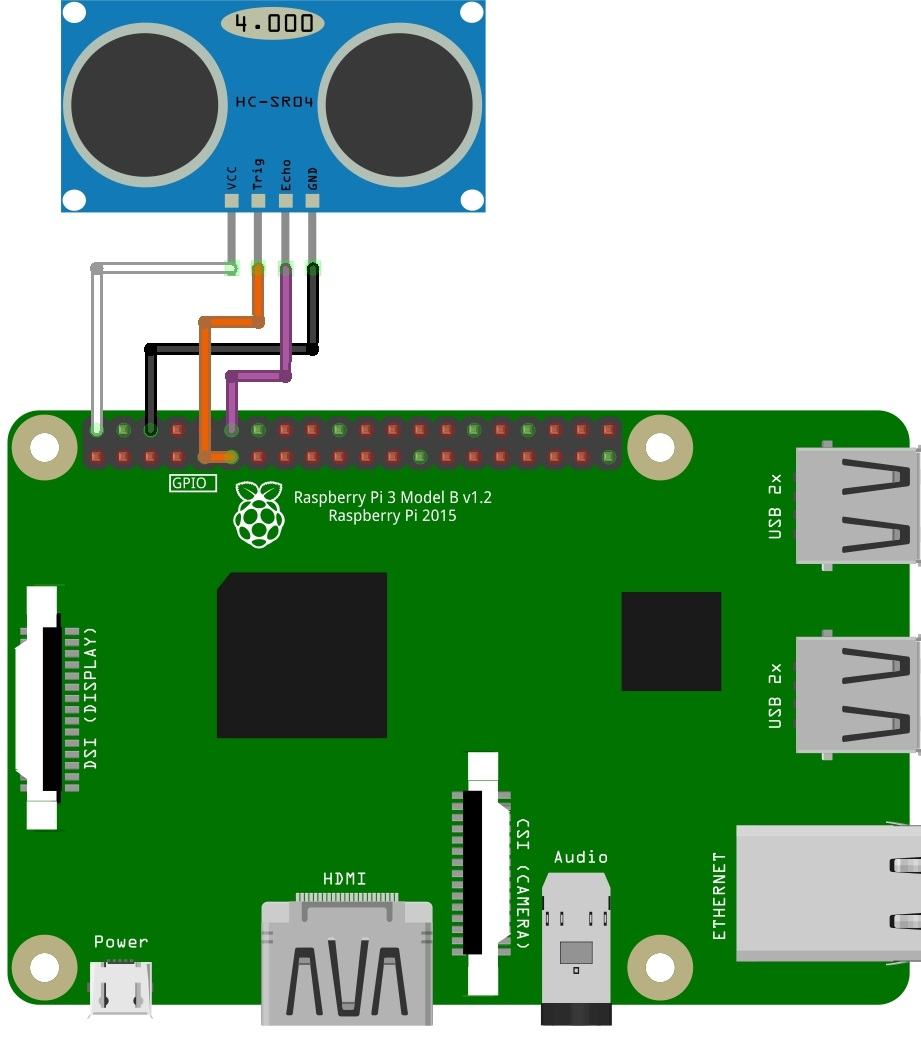
\includegraphics[height=7cm, width=0.5\textwidth, center]{images/skematik_ultra.jpg}
    \caption{Ragkaian Raspberry Pi dan Ultrasonik}
    \label{fig:skematikUltrasonik}
\end{figure}

Gambar ~\ref{fig:skematikUltrasonik} merupakan gambar rangkaian Raspberry Pi dan sensor ultrasonik. Sensor ultrasonik berfungsi sebagai indikator untuk menutup palang parkir. Apabila didepan sensor ultrasonik masih ada kendaraan, maka palang parkir masih akan terbuka, sebaliknya apabila didepan sensor sudah tidak ada kendaraan, maka palang parkir akan menutup. Sensor ultrasonik yang digunakan adalah HC-SR04 yang mempunyai 4 pin yaitu pin \textit{ground} (-), pin \textit{echo}, pin \textit{trigger}, dan pin vcc (+). Untuk pin pada Raspberry Pi dihubungkan pada sensor HC-SR04 dapat dilihat pada tabel ~\ref{table:tableUltrasonic}.\newline

\begin{atable}
    \caption{Rangkaian pin Ultrasonik ke Raspberry Pi}
    \label{table:tableUltrasonic}
    \csvreader[
        % column count = 11,
        respect underscore=true,
        tabular=cc,
        head to column names,
        before table=\rowcolors{2}{gray!15}{gray!30},
        table head= \rowcolor{gray!50!black} 
            \color{white} ULTRASONIK & 
            \color{white} RASPBERRY PI 
            \\]
        {tables/tableultrasonic.csv}
        {
            ULTRASONIC=\ULTRASONIC, 
            RASPBERRYPI=\RASPBERRYPI}
        {
            \ULTRASONIC & 
            \RASPBERRYPI}
\end{atable}

Berikut ini pengujian yang dilakukan pada sensor ultrasonik untuk mengukur tinggat kesalahan jarak yang diukur oleh sensor ultrasonik dibandingkan jarak sebenarnya dengan pengukuran secara manual: \newline \newline

% \begin{table}[H]
%     \caption{Hasil uji jarak baca servo}
%     \label{table:tableUjiServo}
%     \begin{tabular}{cccccccccc}
%     \hline
%     \multirow{3}{*}{\begin{tabular}[c]{@{}c@{}}Pengukuran \\ Manual\end{tabular}} & \multicolumn{3}{c}{\begin{tabular}[c]{@{}c@{}}Pengukuran \\ Sensor (cm)\end{tabular}} & \multicolumn{3}{c}{\begin{tabular}[c]{@{}c@{}}Selisih \\ Pengukuran (cm)\end{tabular}} & \multicolumn{3}{c}{\begin{tabular}[c]{@{}c@{}}Persentase \\ Kesalahan(\%)\end{tabular}} \\ \cline{2-10} 
%                                                                                   & \multicolumn{3}{c|}{Pengukuran ke-}                                                   & \multicolumn{3}{c|}{Pengukuran ke-}                                                    & \multicolumn{3}{c|}{Pengukuran ke-}                                                     \\ \cline{2-10} 
%                                                                                   & \multicolumn{1}{c|}{1}      & \multicolumn{1}{c|}{2}     & \multicolumn{1}{c|}{3}     & \multicolumn{1}{c|}{1}      & \multicolumn{1}{c|}{2}      & \multicolumn{1}{c|}{3}     & \multicolumn{1}{c|}{1}      & \multicolumn{1}{c|}{2}      & \multicolumn{1}{c|}{3}      \\ \hline
%     \multicolumn{1}{|c|}{2}                                                       & \multicolumn{1}{c|}{2}      & \multicolumn{1}{c|}{2}     & \multicolumn{1}{c|}{2}     & \multicolumn{1}{c|}{0}      & \multicolumn{1}{c|}{0}      & \multicolumn{1}{c|}{0}     & \multicolumn{1}{c|}{0}      & \multicolumn{1}{c|}{0}      & \multicolumn{1}{c|}{0}      \\ \hline
%     \multicolumn{1}{|c|}{6}                                                       & \multicolumn{1}{c|}{6}      & \multicolumn{1}{c|}{6}     & \multicolumn{1}{c|}{6}     & \multicolumn{1}{c|}{0}      & \multicolumn{1}{c|}{0}      & \multicolumn{1}{c|}{0}     & \multicolumn{1}{c|}{0}      & \multicolumn{1}{c|}{0}      & \multicolumn{1}{c|}{0}      \\ \hline
%     \multicolumn{1}{|c|}{15}                                                      & \multicolumn{1}{c|}{15}     & \multicolumn{1}{c|}{15}    & \multicolumn{1}{c|}{15}    & \multicolumn{1}{c|}{0}      & \multicolumn{1}{c|}{0}      & \multicolumn{1}{c|}{0}     & \multicolumn{1}{c|}{0}      & \multicolumn{1}{c|}{0}      & \multicolumn{1}{c|}{0}      \\ \hline
%     \multicolumn{1}{|c|}{20}                                                      & \multicolumn{1}{c|}{20}     & \multicolumn{1}{c|}{19}    & \multicolumn{1}{c|}{19}    & \multicolumn{1}{c|}{0}      & \multicolumn{1}{c|}{1}      & \multicolumn{1}{c|}{1}     & \multicolumn{1}{c|}{0}      & \multicolumn{1}{c|}{5}      & \multicolumn{1}{c|}{5}      \\ \hline
%     \multicolumn{1}{|c|}{30}                                                      & \multicolumn{1}{c|}{29}     & \multicolumn{1}{c|}{29}    & \multicolumn{1}{c|}{29}    & \multicolumn{1}{c|}{1}      & \multicolumn{1}{c|}{1}      & \multicolumn{1}{c|}{1}     & \multicolumn{1}{c|}{3}      & \multicolumn{1}{c|}{3}      & \multicolumn{1}{c|}{3}      \\ \hline
%     \multicolumn{1}{|c|}{40}                                                      & \multicolumn{1}{c|}{38}     & \multicolumn{1}{c|}{39}    & \multicolumn{1}{c|}{38}    & \multicolumn{1}{c|}{2}      & \multicolumn{1}{c|}{1}      & \multicolumn{1}{c|}{2}     & \multicolumn{1}{c|}{5}      & \multicolumn{1}{c|}{3}      & \multicolumn{1}{c|}{5}      \\ \hline
%     \multicolumn{1}{|c|}{50}                                                      & \multicolumn{1}{c|}{49}     & \multicolumn{1}{c|}{49}    & \multicolumn{1}{c|}{49}    & \multicolumn{1}{c|}{1}      & \multicolumn{1}{c|}{1}      & \multicolumn{1}{c|}{1}     & \multicolumn{1}{c|}{2}      & \multicolumn{1}{c|}{2}      & \multicolumn{1}{c|}{2}      \\ \hline
%     \multicolumn{1}{|c|}{60}                                                      & \multicolumn{1}{c|}{57}     & \multicolumn{1}{c|}{56}    & \multicolumn{1}{c|}{57}    & \multicolumn{1}{c|}{3}      & \multicolumn{1}{c|}{4}      & \multicolumn{1}{c|}{3}     & \multicolumn{1}{c|}{5}      & \multicolumn{1}{c|}{7}      & \multicolumn{1}{c|}{5}      \\ \hline
%     \multicolumn{1}{|c|}{70}                                                      & \multicolumn{1}{c|}{68}     & \multicolumn{1}{c|}{69}    & \multicolumn{1}{c|}{68}    & \multicolumn{1}{c|}{2}      & \multicolumn{1}{c|}{1}      & \multicolumn{1}{c|}{2}     & \multicolumn{1}{c|}{3}      & \multicolumn{1}{c|}{1}      & \multicolumn{1}{c|}{3}      \\ \hline
%     \multicolumn{1}{|c|}{80}                                                      & \multicolumn{1}{c|}{78}     & \multicolumn{1}{c|}{78}    & \multicolumn{1}{c|}{78}    & \multicolumn{1}{c|}{2}      & \multicolumn{1}{c|}{2}      & \multicolumn{1}{c|}{2}     & \multicolumn{1}{c|}{3}      & \multicolumn{1}{c|}{3}      & \multicolumn{1}{c|}{3}      \\ \hline
%     \multicolumn{1}{|c|}{90}                                                      & \multicolumn{1}{c|}{89}     & \multicolumn{1}{c|}{90}    & \multicolumn{1}{c|}{88}    & \multicolumn{1}{c|}{1}      & \multicolumn{1}{c|}{0}      & \multicolumn{1}{c|}{2}     & \multicolumn{1}{c|}{1}      & \multicolumn{1}{c|}{0}      & \multicolumn{1}{c|}{2}      \\ \hline
%     \multicolumn{1}{|c|}{100}                                                     & \multicolumn{1}{c|}{96}     & \multicolumn{1}{c|}{97}    & \multicolumn{1}{c|}{96}    & \multicolumn{1}{c|}{4}      & \multicolumn{1}{c|}{3}      & \multicolumn{1}{c|}{4}     & \multicolumn{1}{c|}{4}      & \multicolumn{1}{c|}{3}      & \multicolumn{1}{c|}{4}      \\ \hline
%     \multicolumn{1}{|c|}{110}                                                     & \multicolumn{1}{c|}{107}    & \multicolumn{1}{c|}{107}   & \multicolumn{1}{c|}{108}   & \multicolumn{1}{c|}{3}      & \multicolumn{1}{c|}{3}      & \multicolumn{1}{c|}{2}     & \multicolumn{1}{c|}{3}      & \multicolumn{1}{c|}{3}      & \multicolumn{1}{c|}{2}      \\ \hline
%     \multicolumn{1}{|c|}{120}                                                     & \multicolumn{1}{c|}{115}    & \multicolumn{1}{c|}{114}   & \multicolumn{1}{c|}{115}   & \multicolumn{1}{c|}{5}      & \multicolumn{1}{c|}{6}      & \multicolumn{1}{c|}{5}     & \multicolumn{1}{c|}{4}      & \multicolumn{1}{c|}{5}      & \multicolumn{1}{c|}{4}      \\ \hline
%     \multicolumn{7}{c}{Rata-rata kesalahan}                                                                                                                                                                                                                        & 2,34                        & 2,44                        & 2,71                        \\ \hline
%     \end{tabular}
% \end{table}

\begin{atable} 
    \caption{Hasil uji jarak baca servo}
    \label{table:tableUjiServo}
    \begin{tabular}{|c|c|c|c|c|c|c|c|c|c|}
    \hline
    \multirow{3}{2cm}{Pengukuran Manual(cm)} & \multicolumn{3}{c|}{Pengukuran Sensor(cm)} & \multicolumn{3}{c|}{Selisih Pengukuran(cm)} & \multicolumn{3}{c|}{Persentase Kesalahan(\%)} \\ \cline{2-10} 
                                       & \multicolumn{3}{c|}{Pengukuran ke-}         & \multicolumn{3}{c|}{Pengukuran ke-}          & \multicolumn{3}{c|}{Pengukuran ke-}       \\ \cline{2-10} 
                                       & 1             & 2            & 3            & 1             & 2             & 3            & 1            & 2            & 3           \\ \hline
    2                                  & 2             & 2            & 2            & 0             & 0             & 0            & 0            & 0            & 0           \\ \hline
    6                                  & 6             & 6            & 6            & 0             & 0             & 0            & 0            & 0            & 0           \\ \hline
    15                                 & 15            & 15           & 15           & 0             & 0             & 0            & 0            & 0            & 0           \\ \hline
    20                                 & 20            & 19           & 19           & 0             & 1             & 1            & 0            & 5            & 5           \\ \hline
    30                                 & 29            & 29           & 29           & 1             & 1             & 1            & 3            & 3            & 3           \\ \hline
    40                                 & 38            & 39           & 38           & 2             & 1             & 2            & 5            & 3            & 5           \\ \hline
    50                                 & 49            & 49           & 49           & 1             & 1             & 1            & 2            & 2            & 2           \\ \hline
    60                                 & 57            & 56           & 57           & 3             & 4             & 3            & 5            & 7            & 5           \\ \hline
    70                                 & 68            & 69           & 68           & 2             & 1             & 2            & 3            & 1            & 3           \\ \hline
    80                                 & 78            & 78           & 78           & 2             & 2             & 2            & 3            & 3            & 3           \\ \hline
    90                                 & 89            & 90           & 88           & 1             & 0             & 2            & 1            & 0            & 2           \\ \hline
    100                                & 96            & 97           & 96           & 4             & 3             & 4            & 4            & 3            & 4           \\ \hline
    110                                & 107           & 107          & 108          & 3             & 3             & 2            & 3            & 3            & 2           \\ \hline
    120                                & 115           & 114          & 115          & 5             & 6             & 5            & 4            & 5            & 4           \\ \hline
    \multicolumn{7}{|c|}{Rata-rata kesalahan}                                                                                       & 2,34         & 2,44         & 2,71        \\ \hline
    \end{tabular}
\end{atable}

Berdasarkan data hasil pengujian sensor ultrasonik pada tabel ~\ref{table:tableUjiServo}, pengambilan data dilakukan sebanyak empat belas kali dengan tiga kali pengukuran, didapatkan hasil yang berbeda antara pengukuran manual yang menggunakan penggaris dengan pengukuran oleh sensor. Dari data hasil pengukuran yang pertama didapatbahwa terdapat selisih jarak hasil pengujian oleh sensor dengan jarak sebenarnya, dilakukan pengukuran dengan rentang jarak dari 2 cm sampai 120 cm yang dimana untuk pengukuran 2 cm sampai 15 cm tidak ada selisih antara pengukuran manual dan pengukuran sensor. Pada jarak 20 cm tidak ada selisih untuk pengukuran pertama, sedangkan pengukuran kedua dan ketiga terdapat selisih sebesar 1 cm. Pada jarak 30 cm terdapat selisih 1 cm untuk semua pengukuran. Pada jarak 40 cm selisih pada pengukuran pertama sebesar 2 cm, kedua sebesar 1 cm, dan ketiga sebesar 2 cm. Pada jarak 50 cm dan 60 cm terdapat selisih sebesar 2 cm pada setiap pengukuran. Pada jara 70 cm selisih pada pengukuran pertama sebesar 2 cm, kedua sebesar 1 cm, dan ketiga sebesar 2 cm. Pada jarak 80 cm dan 90 cm terdapat selisih sebesar 3 cm pada setiap pengukuran. Pada jarak 100 cm dan 110 cm terdapat selisih sebesar 4 cm pada setiap pengukuran. Pada jarak 120 cm selisih pada pengukuran pertama sebesar 5 cm, kedua sebesar 6 cm, dan ketiga sebesar 5 cm.

Berdasarkan data hasil pengujian pada tabel menunjukan bahwa semakin jauh jarak yang diukur, semakin besar kesalahan jarak yang diukur oleh sensor dari jarak sebenarnya. Perbedaan jarak hasil pengujian sensor dengan jarak sesungguhnya dapat disebabkan oleh adanya \textit{noise} atau permukaan jarak yang diukur tidak rata.

Berikut ini rumus serta perhitungan yang digunakan untuk menghitungpersentase kesalahan dan rata-rata kesalahan, dari perbandingan pengukuran jarakantara sensor dengan manual:

\begin{enumerate}[topsep=0pt,itemsep=0pt,partopsep=0pt, parsep=0pt]
    \item Persentase kesalahan
    \begin{equation}
        \label{eq:persentase-kesalahan}
        \begin{split}
        \%kesalahan = \frac{(jarak manual - jarak sensor)}{jarak manual} x 100\%
        \end{split}
    \end{equation}

    \item Rata-rata kesalahan
    \begin{equation}
        \label{eq:persentase-kesalahan}
        \begin{split}
        \%rata-rata kesalahan = \frac{jarak \% kesalahan}{banyaknya data} 
        \end{split}
    \end{equation}
\end{enumerate}

\subsection{Raspberry Pi dan SG90}
\begin{figure} [H]
    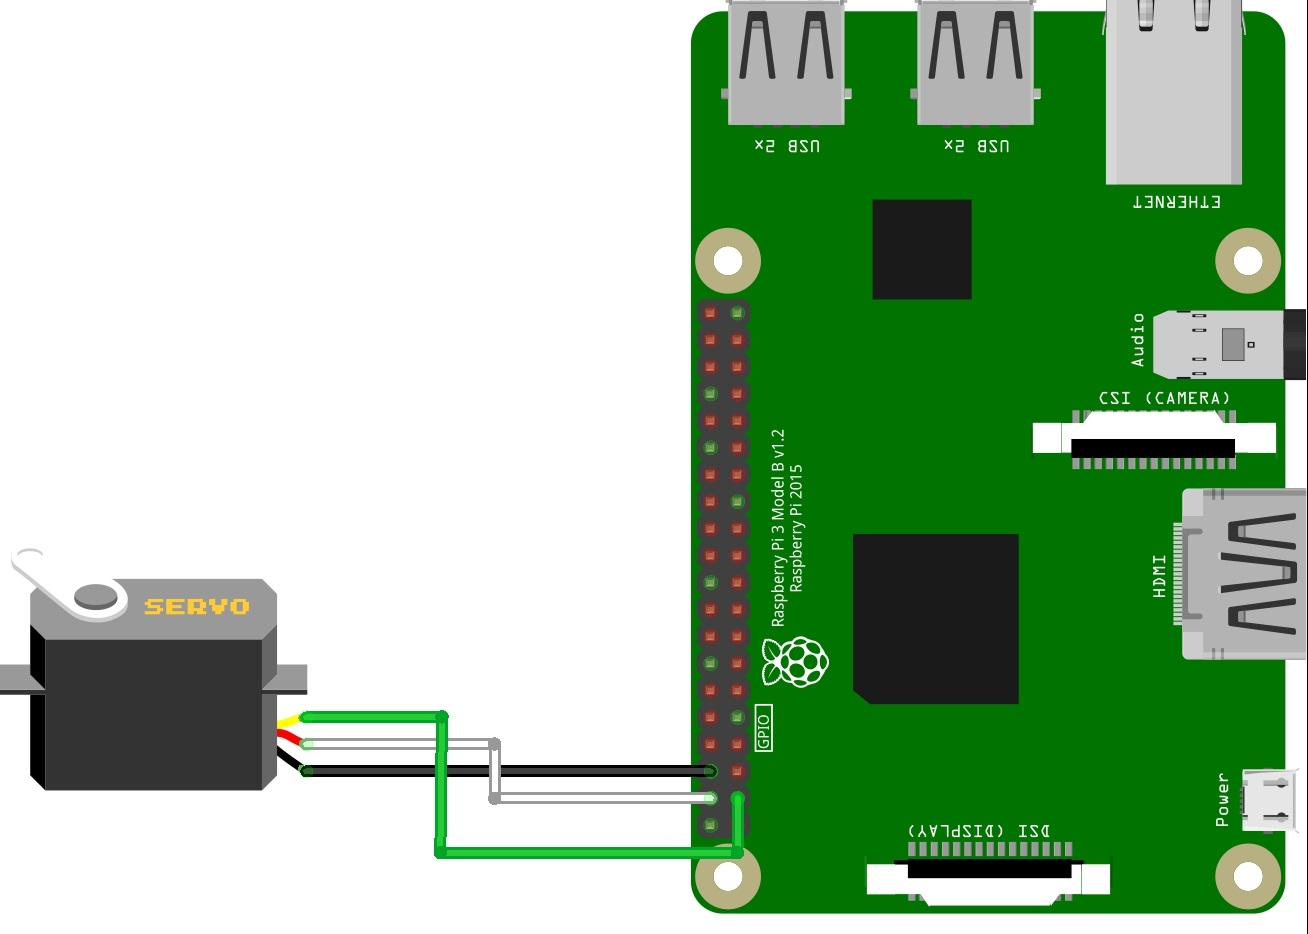
\includegraphics[height=7cm, width=0.6\textwidth, center]{images/skematik_servo.jpg}
    \caption{Ragkaian Raspberry Pi dan Servo}
    \label{fig:skematikServo}
\end{figure}

Pada penelitian ini yang akan berfungsi sebagai palang parkir adalah servo SG90. Servo yang digunakan mempunyai 3 pin yaitu pin \textit{ground} (-), pin pwm, dan pin 5v (+). Untuk pin pada Raspberry Pi dihubungkan pada servo SG90 dapat dilihat pada tabel ~\ref{table:tableServo}.

\begin{atable}
    \caption{Rangkaian pin Servo ke Raspberry Pi}
    \label{table:tableServo}
    \csvreader[
        % column count = 11,
        respect underscore=true,
        tabular=cc,
        head to column names,
        before table=\rowcolors{2}{gray!15}{gray!30},
        table head= \rowcolor{gray!50!black} 
            \color{white} SERVO & 
            \color{white} RASPBERRY PI 
            \\]
        {tables/tableservo.csv}
        {
            SERVO=\SERVO, 
            RASPBERRYPI=\RASPBERRYPI}
        {
            \SERVO & 
            \RASPBERRYPI}
\end{atable}

\subsection{Raspberry Pi dan Button}
\begin{figure} [H]
    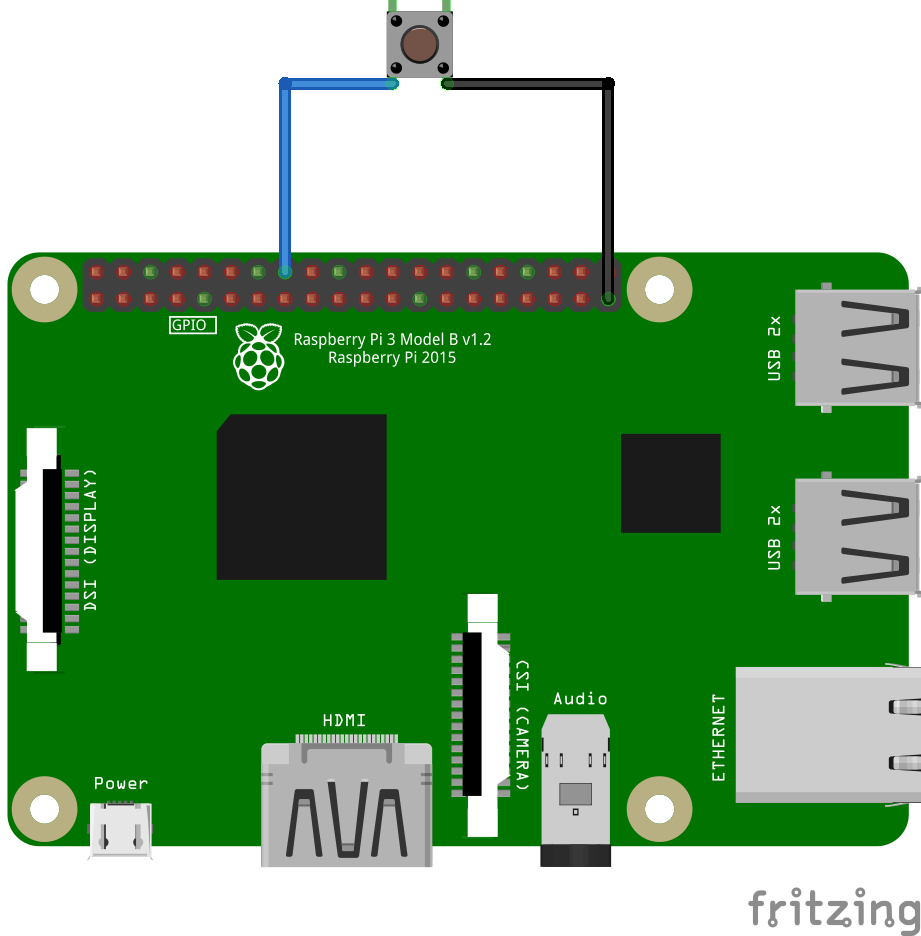
\includegraphics[height=7cm, width=0.6\textwidth, center]{images/skematik_button.png}
    \caption{Ragkaian Raspberry Pi dan Button}
    \label{fig:skematikButton}
\end{figure}
Button berfungsi untuk membuka palang parkir ketika plat kendaraan tidak terbaca. Untuk pin pada Raspberry Pi dihubungkan pada button dapat dilihat pada tabel ~\ref{table:tableButton}.

\begin{atable}
    \caption{Rangkaian pin Button ke Raspberry Pi}
    \label{table:tableButton}
    \csvreader[
        % column count = 11,
        respect underscore=true,
        tabular=cc,
        head to column names,
        before table=\rowcolors{2}{gray!15}{gray!30},
        table head= \rowcolor{gray!50!black} 
            \color{white} Button & 
            \color{white} RASPBERRY PI 
            \\]
        {tables/tablebutton.csv}
        {
            BUTTON=\BUTTON, 
            RASPBERRYPI=\RASPBERRYPI}
        {
            \BUTTON & 
            \RASPBERRYPI}
\end{atable}

\subsection{Raspberry Pi dan Kamera Pi}
\begin{figure} [H]
    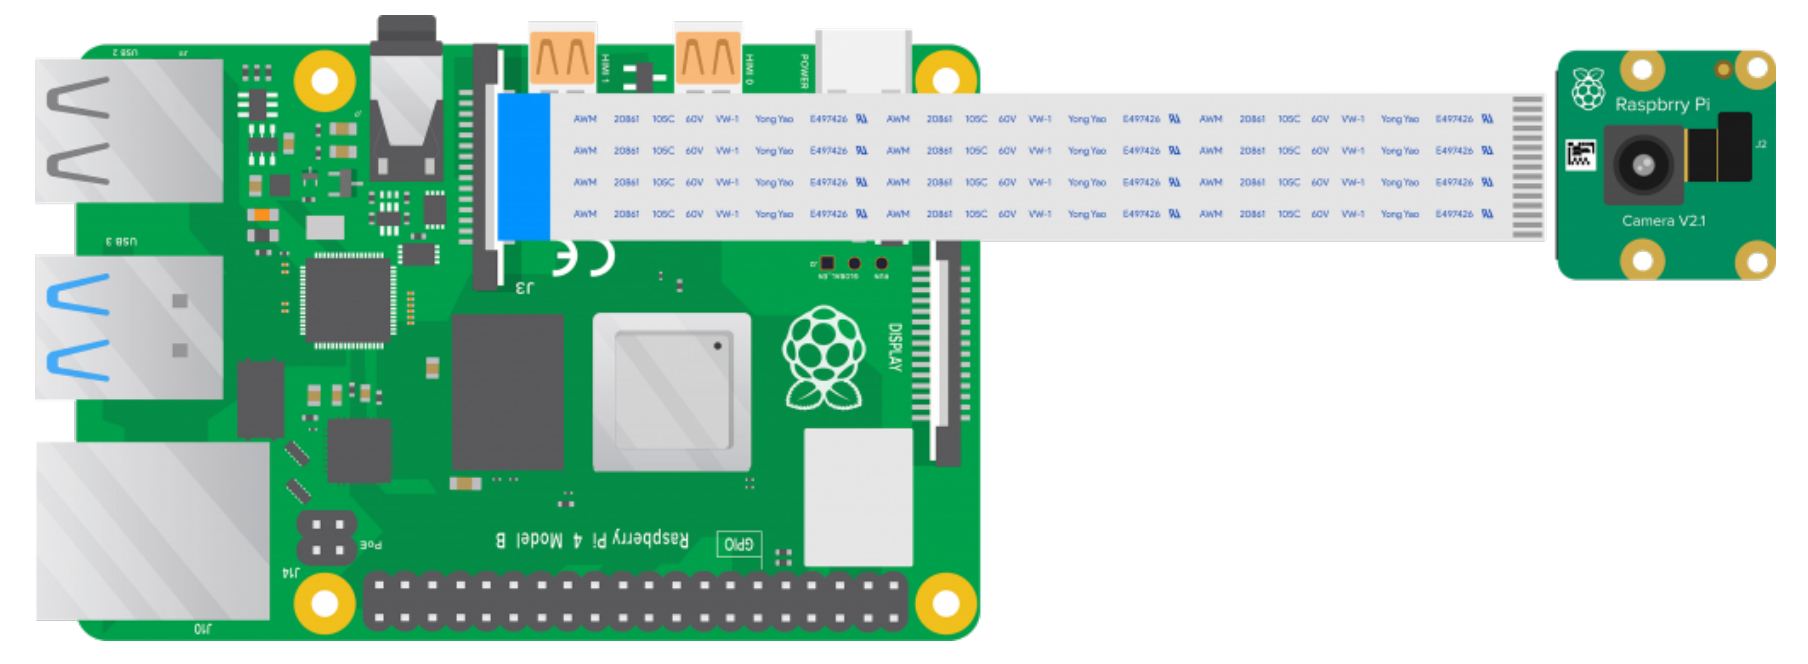
\includegraphics[width=0.85\textwidth, center]{images/skematik-kamera.png}
    \caption{Ragkaian Raspberry Pi dan Kamera}
    \label{fig:skematikKamera}
\end{figure}

Gambar ~\ref{fig:skematikKamera} merupakan gambar skematik Raspberry Pi dengan kamera. Untuk menghubungkan Raspberry Pi dengan kamera cukup dengan menghubungkan kamera dengan port \textit{Camera Serial Interface} (CSI) yang sudah tersedia pada Raspberry Pi. Gambar ~\ref{fig:GambarKameraPi} merupakah hasil foto yang diambil oleh kamera Pi.

\begin{figure} [H]
    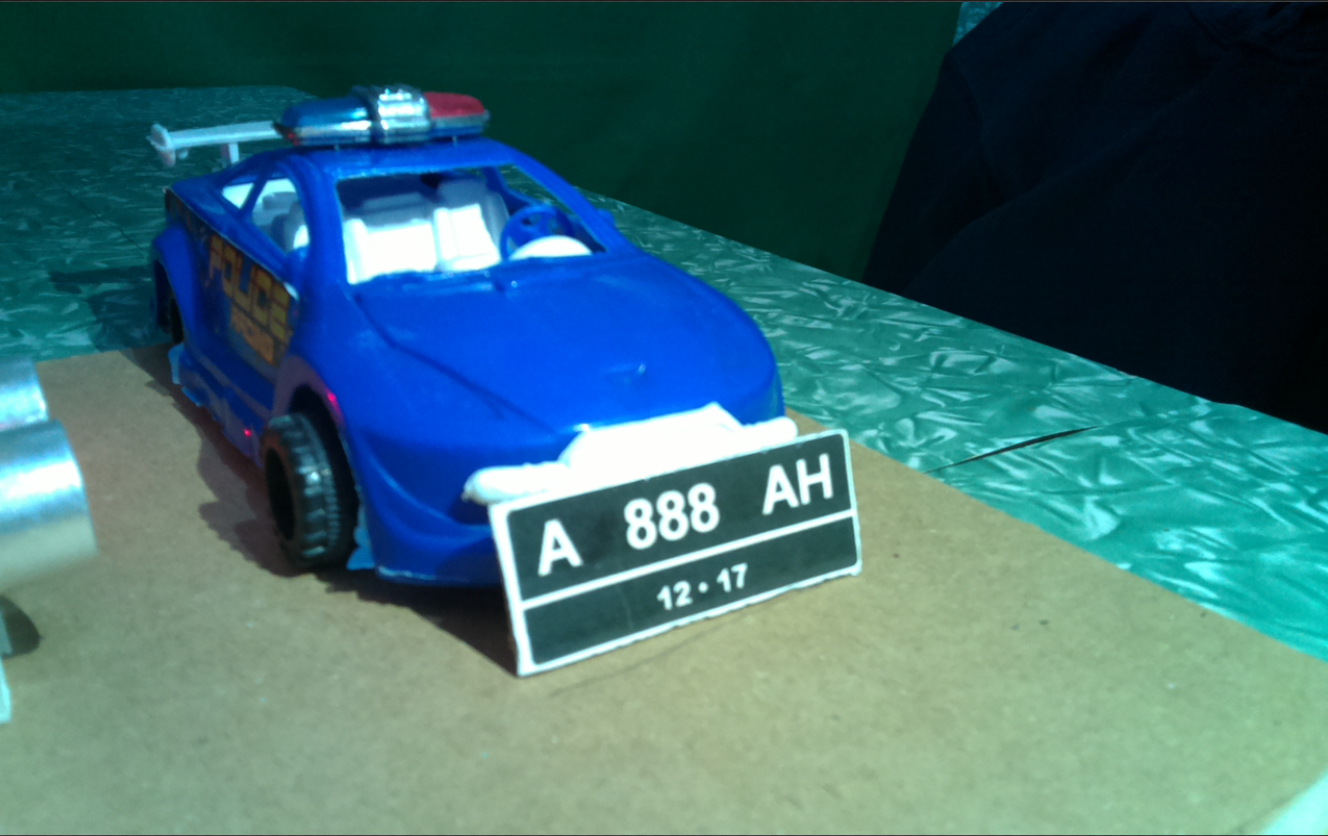
\includegraphics[width=0.85\textwidth, center]{images/Hasil Gambar Kamera Pi.png}
    \caption{Hasil Foto Kamera Pi}
    \label{fig:GambarKameraPi}
\end{figure}

Foto yang diambil oleh kamera akan di proses untuk mengambil nomor plat kendaraan. Pengambilan nomor plat kendaraan menggunakan API (\textit{Aplication Programming Interface}) yang disediakan oleh \textit{platerecognizer.com}. Foto yang telah diambil oleh kamera akan dikirim dengan cara mengakses API \textit{platerecognizer.com} yang telah dihubungkan. Setelah berhasil mengakses alamat API, permintaan tersebut akan diteruskan ke server \textit{platerecognizer.com}. Jadi, API akan memberitahukan bahwa aplikasi membutuhkan data nomor pelat sesuai gambar yang dikirim. Setelah memproses foto dan menemukan data yang diinginkan, server kembali menghubungi API. Data tersebut berupa nomor plat kendaraan. Selanjutnya, API meneruskan informasi dari server ke aplikasi kita.

% \subsection{Hasil Perancangan Perangkat Lunak}

\section{Hasil Rancangan Aplikasi Web}
Pada penelitian ini menggunakan web sebagai \textit{user interface}. Web yang digunakan dibuat dengan bahasa pemrograman python dan Flask sebagai \textit{framework}nya.

\subsection{\textit{Entity relationship Diagram}}
\begin{figure} [H]
    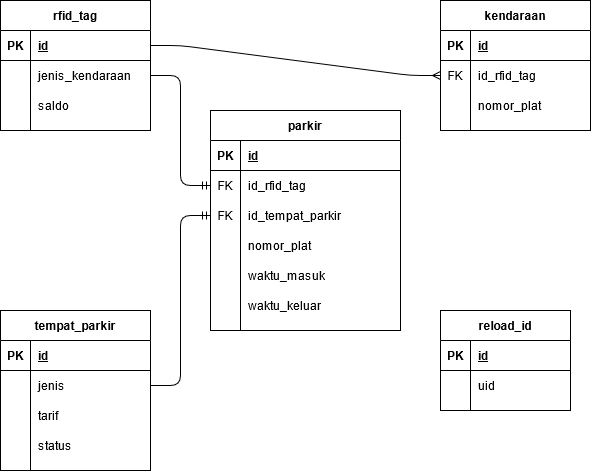
\includegraphics[width=0.85\textwidth, center]{images/er diagram.png}
    \caption{ERD}
    \label{fig:erd}
\end{figure}

Pada gambar ~\ref{fig:erd}, dapat dilihat terdapat 4 tabel yang saling berelasi antar tabel lain dan 1 tabel yang tidak mempunyai relasi antar tabel lain.

\subsection{Struktur \textit{Database}}
Nama \textit{database} : skripsi

Pada \textit{database} aplikasi ini, tabel dibagi menjadi 5 tabel sebagai berikut:

\begin{enumerate}[topsep=0pt,itemsep=0pt,partopsep=0pt, parsep=0pt]
    \item Tabel rfid\_tag

    Nama Tabel : rfid\_tag

    \textit{Primary Key} : id

    \begin{atable}
        \caption{rfid\_tag}
        \label{table:db_rfid_tag}
        \csvreader[
            % column count = 11,
            respect underscore=true,
            tabular=cc,
            head to column names,
            before table=\rowcolors{2}{gray!15}{gray!30},
            table head= \rowcolor{gray!50!black} 
                \color{white} \textit{Coloumn} & 
                \color{white} \textit{Type} 
                \\]
            {tables/db_rfid_tag.csv}
            {
                Coloumn=\Coloumn, 
                Type=\Type}
            {
                \Coloumn & 
                \Type}
    \end{atable}

    Atribut \textit{id} pada tabel rfid\_tag berfungsi sebagai kunci utama. Atribut jenis\_kendaraan digunakan untuk menentukan jenis kendaraan yang digunakan oleh pengemudi. Atribut saldo digunakan untuk menyimpan saldo dari pengemudi.

    \item Tabel tempat\_parkir

    Nama Tabel : tempat\_parkir

    \textit{Primary Key} : id

    \begin{table} [H]
        \centering
        \caption{tempat\_parkir}
        \label{table:db_tempat_parkir}
        \csvreader[
            % column count = 11,
            respect underscore=true,
            tabular=cc,
            head to column names,
            before table=\rowcolors{2}{gray!15}{gray!30},
            table head= \rowcolor{gray!50!black} 
                \color{white} \textit{Coloumn} & 
                \color{white} \textit{Type} 
                \\]
            {tables/db_tempat_parkir.csv}
            {
                Coloumn=\Coloumn, 
                Type=\Type}
            {
                \Coloumn & 
                \Type}
    \end{table}

    Tabel tempat\_parkir mempunyai atribut \textit{id} yang berfungsi sebagai kunci utama, atribut \textit{id} juga berfungsi sebagai nomor slot tempat parkir. Atribut jenis digunakan untuk menentukan jenis dari slot parkir. Atribut tarif digunakan sebagai tarif per jam dari slot parkir. Atribut status digunakan untuk mengetahui apakah slot sedang tersedia atau terpakai.

    \item Tabel kendaraan

    Nama Tabel : kendaraan

    \textit{Primary Key} : id

    \textit{Foreign Key} : id\_rfid\_tag

    \begin{table} [H]
        \centering 
        \caption{kendaraan}
        \label{table:db_kendaraan}
        \csvreader[
            % column count = 11,
            respect underscore=true,
            tabular=cc,
            head to column names,
            respect underscore=true,
            before table=\rowcolors{2}{gray!15}{gray!30},
            table head= \rowcolor{gray!50!black} 
                \color{white} Coloumn & 
                \color{white} Type
                \\]
            {tables/db_kendaraan.csv}
            {
                Coloumn=\Coloumn, 
                Type=\Type}
            {
                \Coloumn & 
                \Type}
    \end{table}

    Tabel kendaraan mempunyai atribut \textit{id} yang berfungsi sebagai kunci utama. Atribut nomor\_plat berfungsi untuk menyimpan nomor plat pengendara. Atribut id\_rfid\_tag didapat dari tabel rfid\_tag.

    \item Tabel parkir

    Nama Tabel : parkir

    \textit{Primary Key} : id

    \textit{Foreign Key} : id\_rfid\_tag, id\_tempat\_parkir

    \begin{table} [H]
        \centering
        \caption{parkir}
        \label{table:db_parkir}
        \csvreader[
            % column count = 11,
            respect underscore=true,
            tabular=cc,
            head to column names,
            before table=\rowcolors{2}{gray!15}{gray!30},
            table head= \rowcolor{gray!50!black} 
                \color{white} \textit{Coloumn} & 
                \color{white} \textit{Type} 
                \\]
            {tables/db_parkir.csv}
            {
                Coloumn=\Coloumn, 
                Type=\Type}
            {
                \Coloumn & 
                \Type}
    \end{table}

    Tabel kendaraan mempunyai atribut \textit{id} yang berfungsi sebagai kunci utama. Atribut id\_rfid\_tag didapat dari tabel rfid\_tag. Atribut nomor\_plat digunakan untuk menyimpan nomor plat pengendara. Atribut id\_tempat\_parkir didapat dari tabel tempat\_parkir. Atribut waktu\_masuk digunakan untuk mencatat waktu masuk pengendara. Atribut waktu\_keluar digunakan untuk mencatat waktu keluar pengguna.

    \item Tabel \textit{reload\_id}

    Nama Tabel : reload\_id

    \textit{Primary Key} : id

    \begin{table} [H]
        \centering
        \caption{reload\_id}
        \label{table:db_reload_id}
        \csvreader[
            % column count = 11,
            respect underscore=true,
            tabular=cc,
            head to column names,
            before table=\rowcolors{2}{gray!15}{gray!30},
            table head= \rowcolor{gray!50!black} 
                \color{white} \textit{Coloumn} & 
                \color{white} \textit{Type} 
                \\]
            {tables/db_reload_id.csv}
            {
                Coloumn=\Coloumn, 
                Type=\Type}
            {
                \Coloumn & 
                \Type}
    \end{table}

    Tabel reload\_id mempunyai atribut \textit{id} yang berfungsi sebagai kunci utama. Atribut uid digunakan untuk menyimpan id rfid tag.

\end{enumerate}

\subsection{Tampilan Website}
Pada tahap ini dilakukan pengimplementasian aplikasi. Berikut penjelasan mengenai tampilan aplikasi.

\subsubsection{Tampilan \textit{Layout} Parkir}
\begin{figure} [H]
    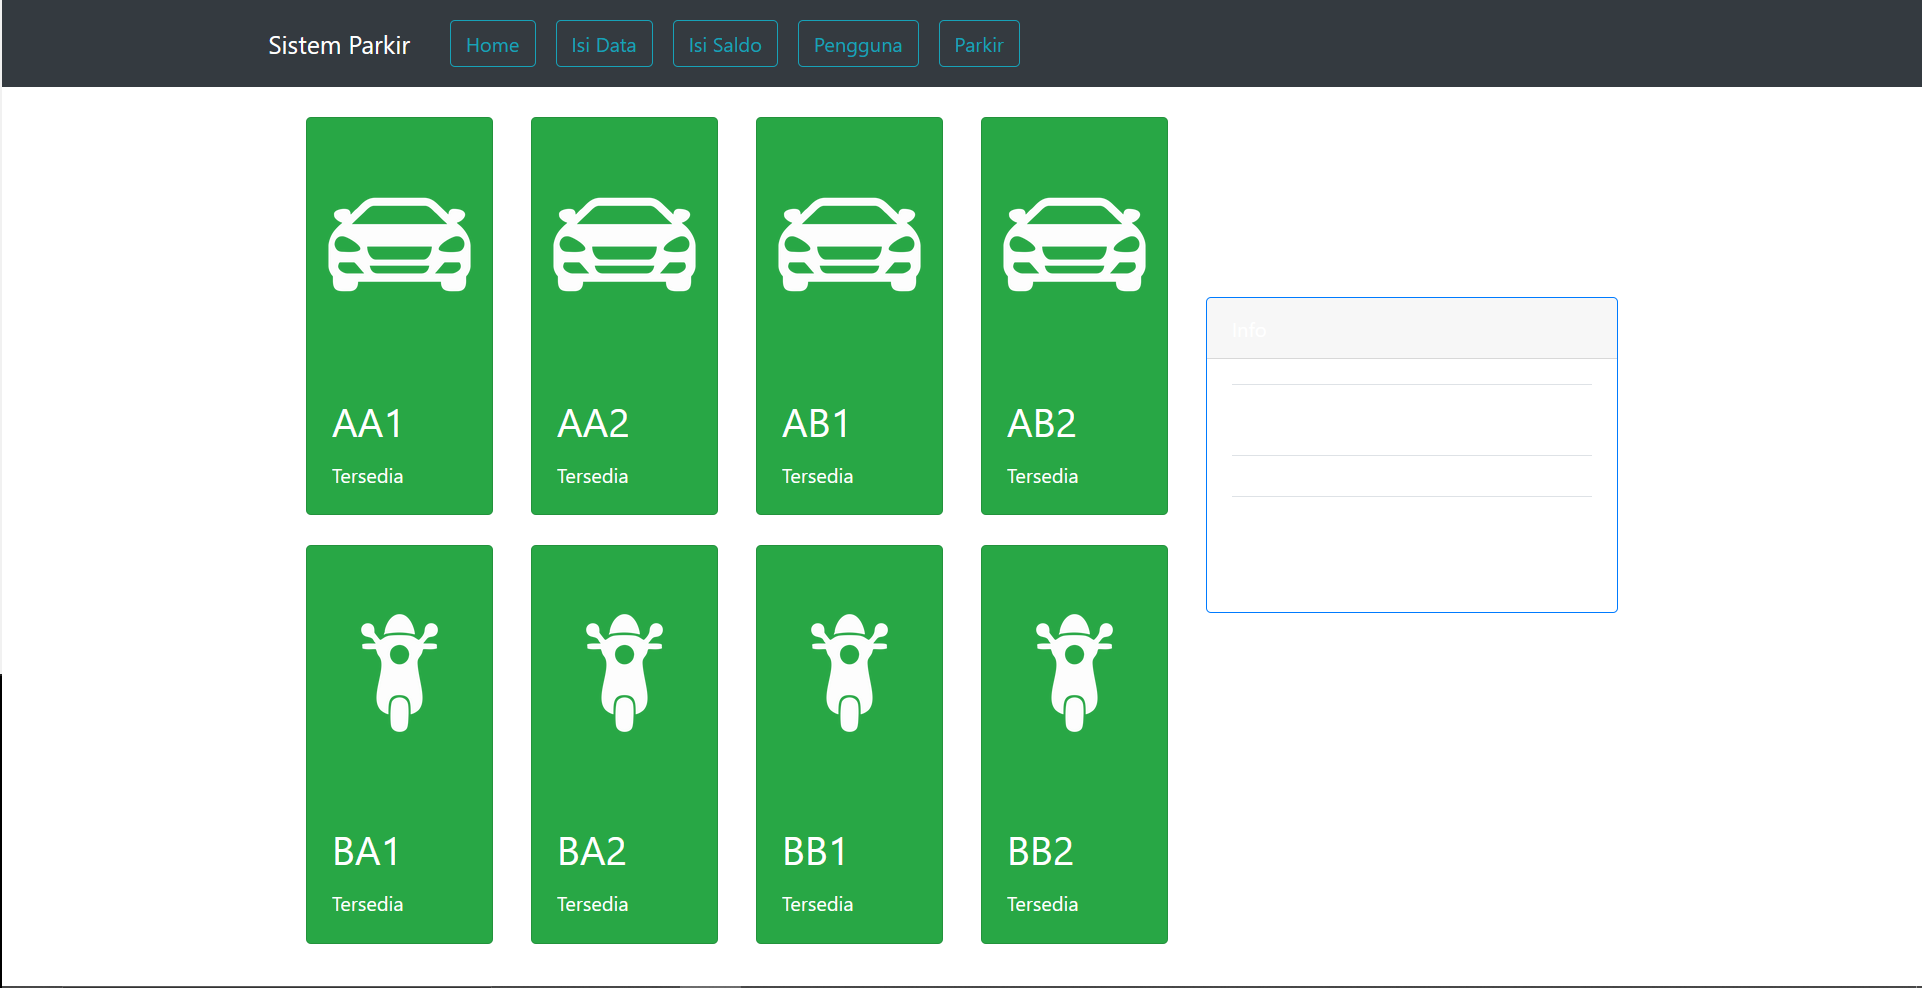
\includegraphics[width=0.85\textwidth, center]{images/web 1 layout parkir.png}
    \caption{\textit{Layout} Parkir}
    \label{fig:web1layout-parkir}
\end{figure}

\textit{Layout} parkir berguna untuk menampilkan informasi mengenai jumlah slot parkir. Pada tampilan kita bisa melihat jumlah slot yang terisi dan terpakai. Pada gambar ~\ref{fig:web1layout-parkir} terlihat jumlah slot parkir ada delapan buah dan semuanya tersedia.\newline

\begin{figure} [H]
    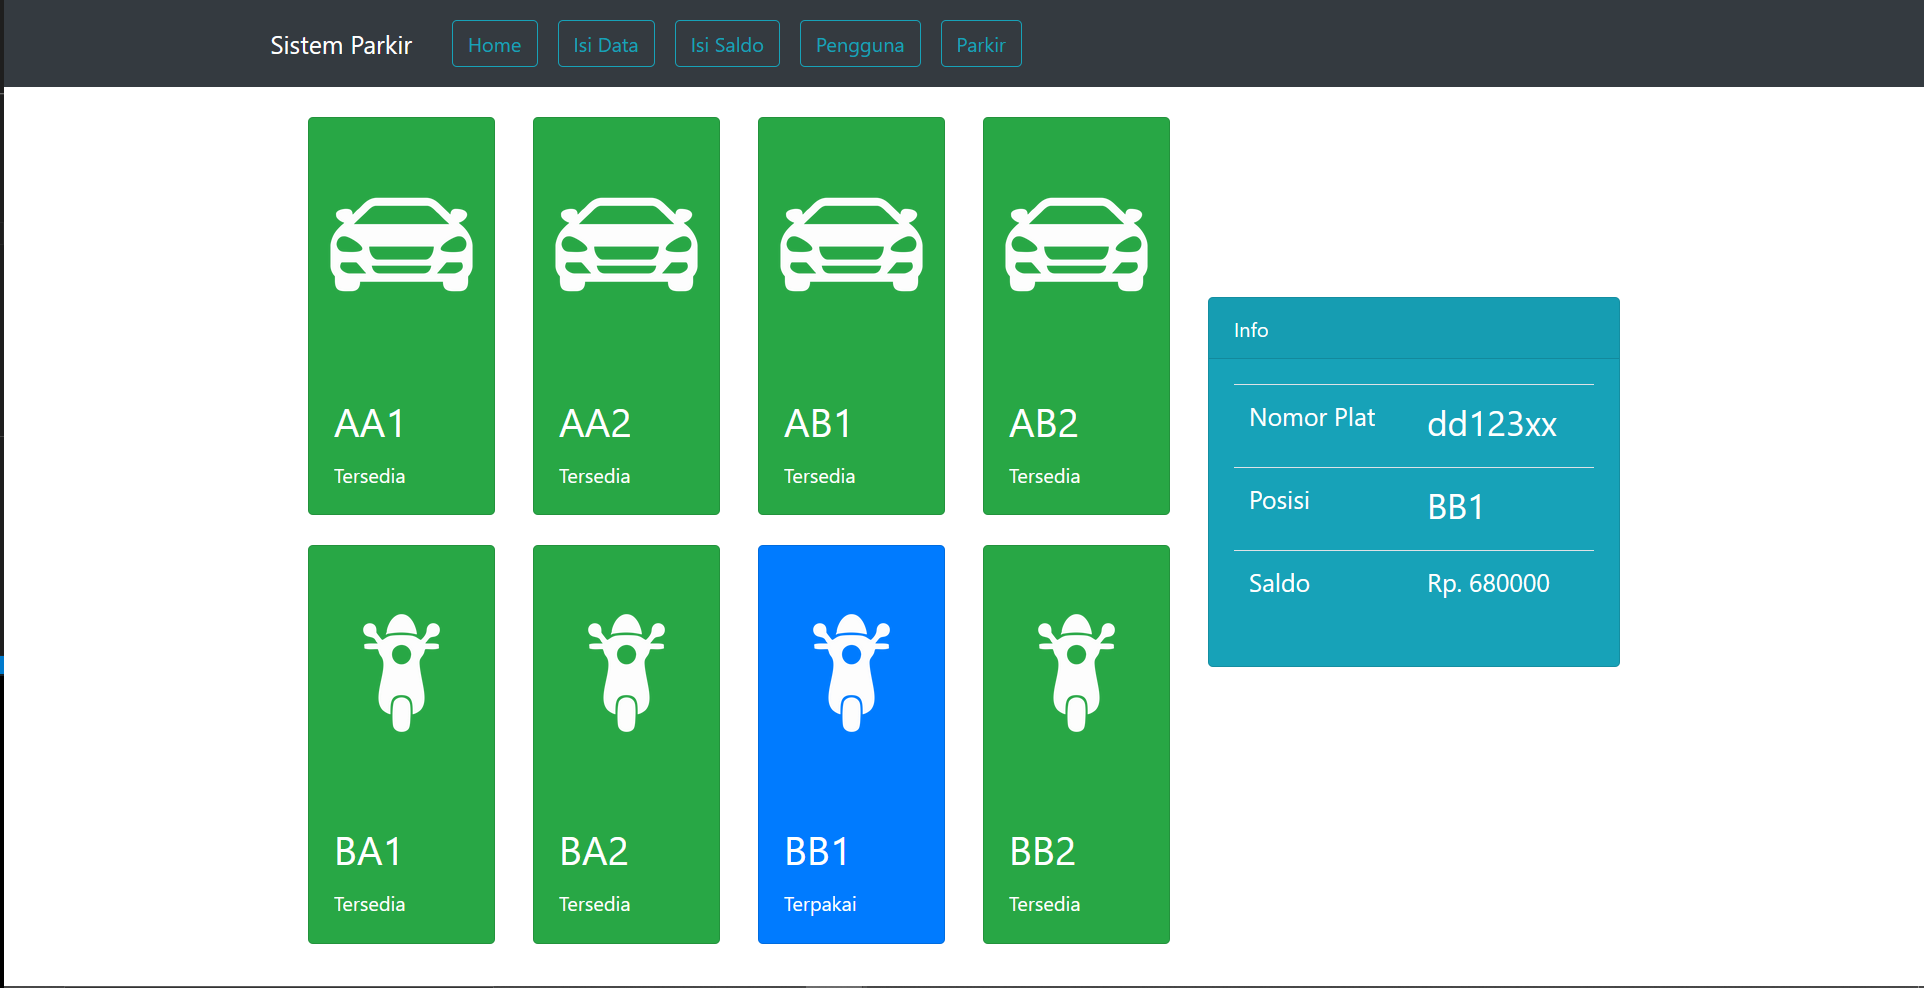
\includegraphics[width=0.85\textwidth, center]{images/web 1 layout parkir baru masuk.png}
    \caption{\textit{Layout} Parkir Saat Pengendara Baru Masuk}
    \label{fig:web1layout-parkir-baru-masuk}
\end{figure}

\begin{figure} [H]
    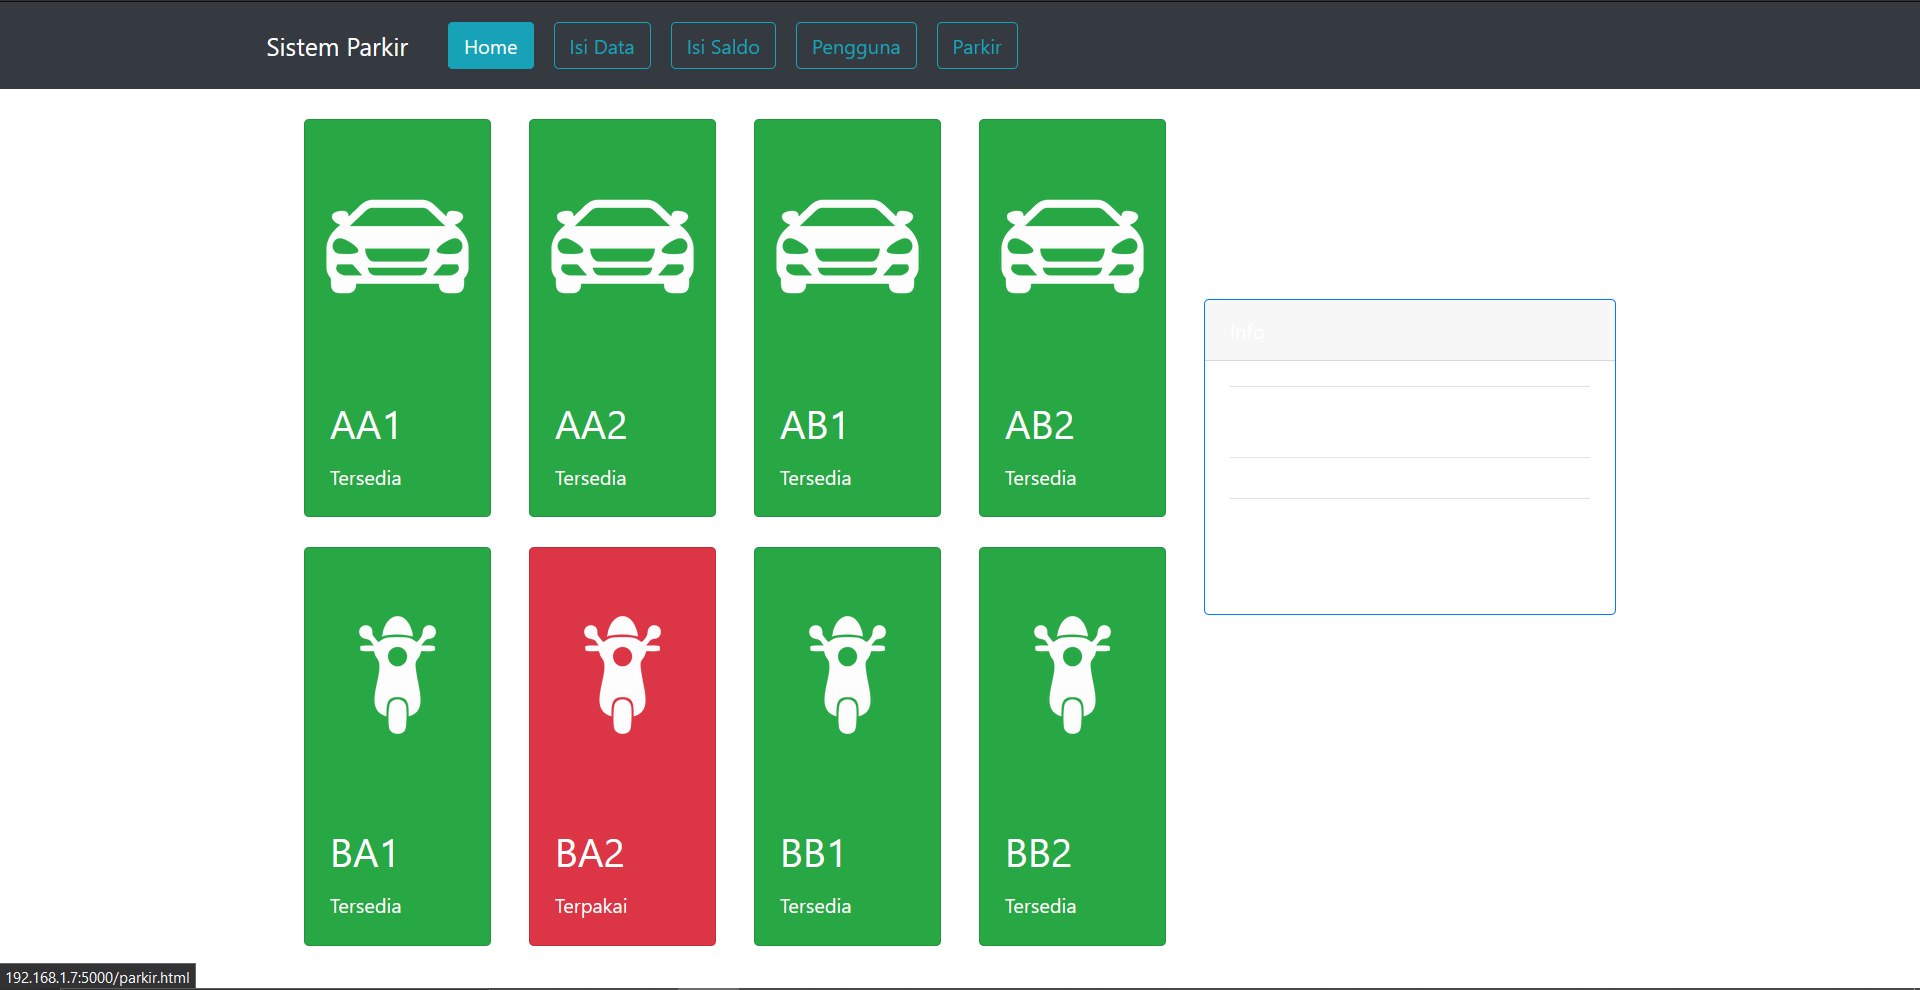
\includegraphics[width=0.85\textwidth, center]{images/web 1 layout parkir ada kendaraan.png}
    \caption{\textit{Layout} Parkir Saat Ada Kendaraan}
    \label{fig:web1layout-parkir-ada-kendaraan}
\end{figure}

Pada gambar ~\ref{fig:web1layout-parkir-baru-masuk} terlihat warna salah satu slot parkir berubah dari warna hijau ke warna biru, ini menunjukan slot yang harus diisi oleh pengendara pada saat baru masuk. Terlihat juga informasi seperti nomor plat, posisi parkir, dan saldo dari pengendara.

Pada gambar ~\ref{fig:web1layout-parkir-ada-kendaraan} terlihat warna slot parkir berubah menjadi warna merah, itu menandakan bahwa slot tersebut sedang terisi.

\subsubsection{Tampilan Isi Data}
\begin{figure} [H]
    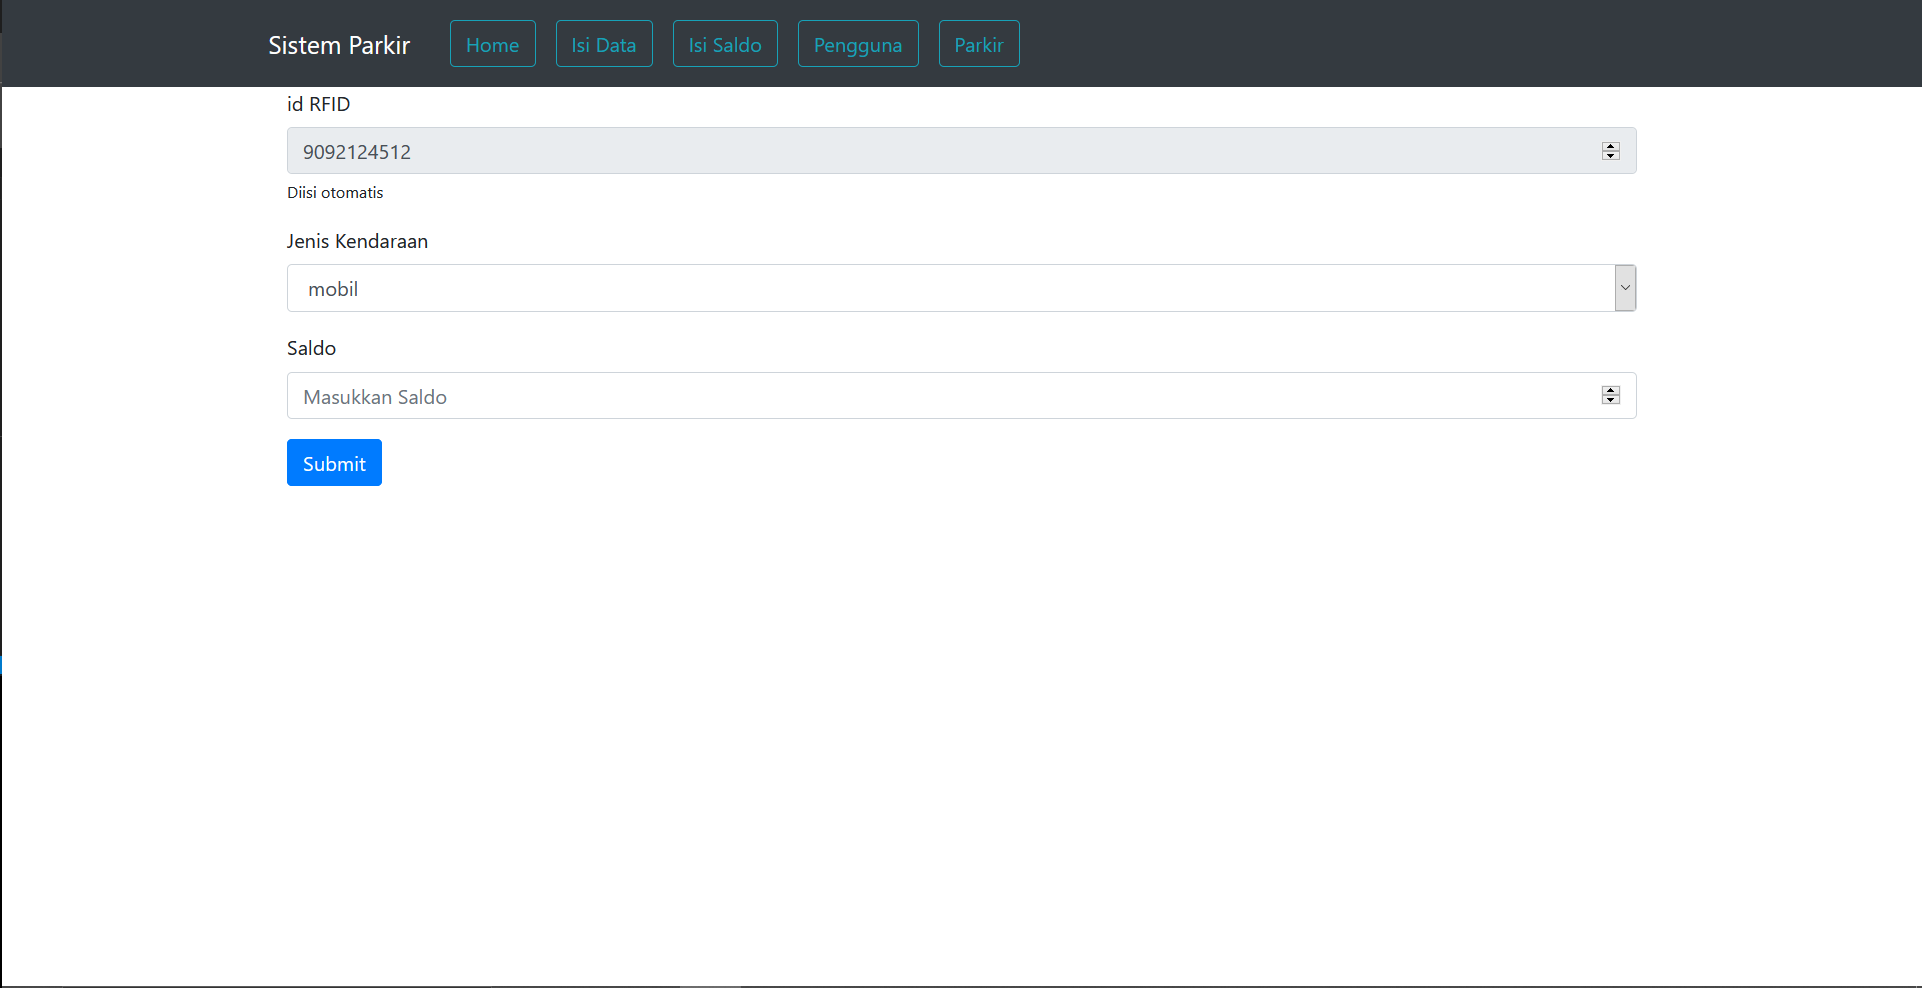
\includegraphics[width=0.85\textwidth, center]{images/web 2 isi data.png}
    \caption{\textit{Form} Isi Data}
    \label{fig:web2isi-data}
\end{figure}

Gambar ~\ref{fig:web2isi-data} merupakan gambar \textit{Form} isi data yang berfungsi untuk memasukkan informasi data pengendara kedalam \textit{database}. Data yang dimasukkan pada \textit{Form} inputan yaitu id RFID, jenis kendaraan, dan saldo. Setelah data diinput maka data akan tersimpan pada \textit{database}.

\subsubsection{Tampilan Isi Saldo}
\begin{figure} [H]
    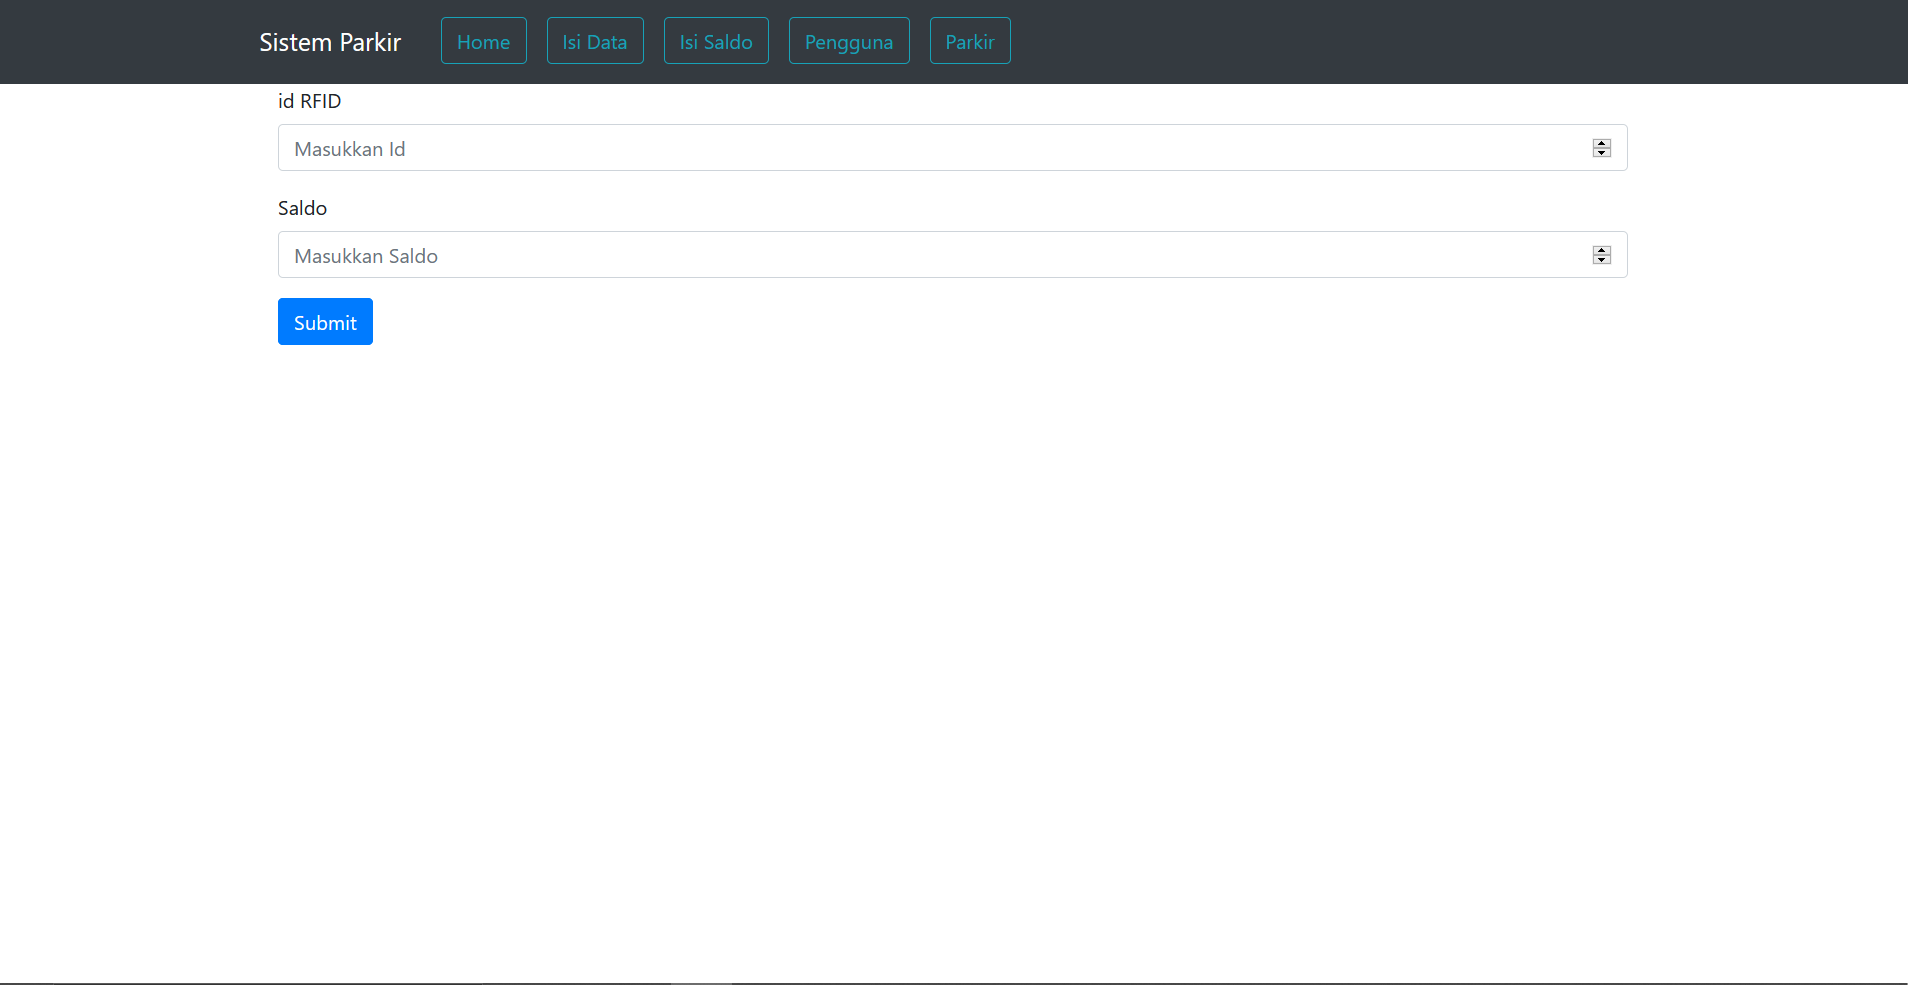
\includegraphics[width=0.85\textwidth, center]{images/web 3 isi saldo.png}
    \caption{\textit{Form} Isi Saldo}
    \label{fig:web3isi-saldo}
\end{figure}

Gambar ~\ref{fig:web3isi-saldo} merupakan gambar \textit{Form} isi saldo yang berfungsi untuk menambahkan saldo pengendara kedalam \textit{database}. Data yang dimasukkan pada \textit{Form} inputan yaitu id RFID dan jumlah saldo yang ingin ditambahkan. Setelah data diinput maka data akan tersimpan pada \textit{database}.

\subsubsection{Tampilan Daftar Pengguna}
\begin{figure} [H]
    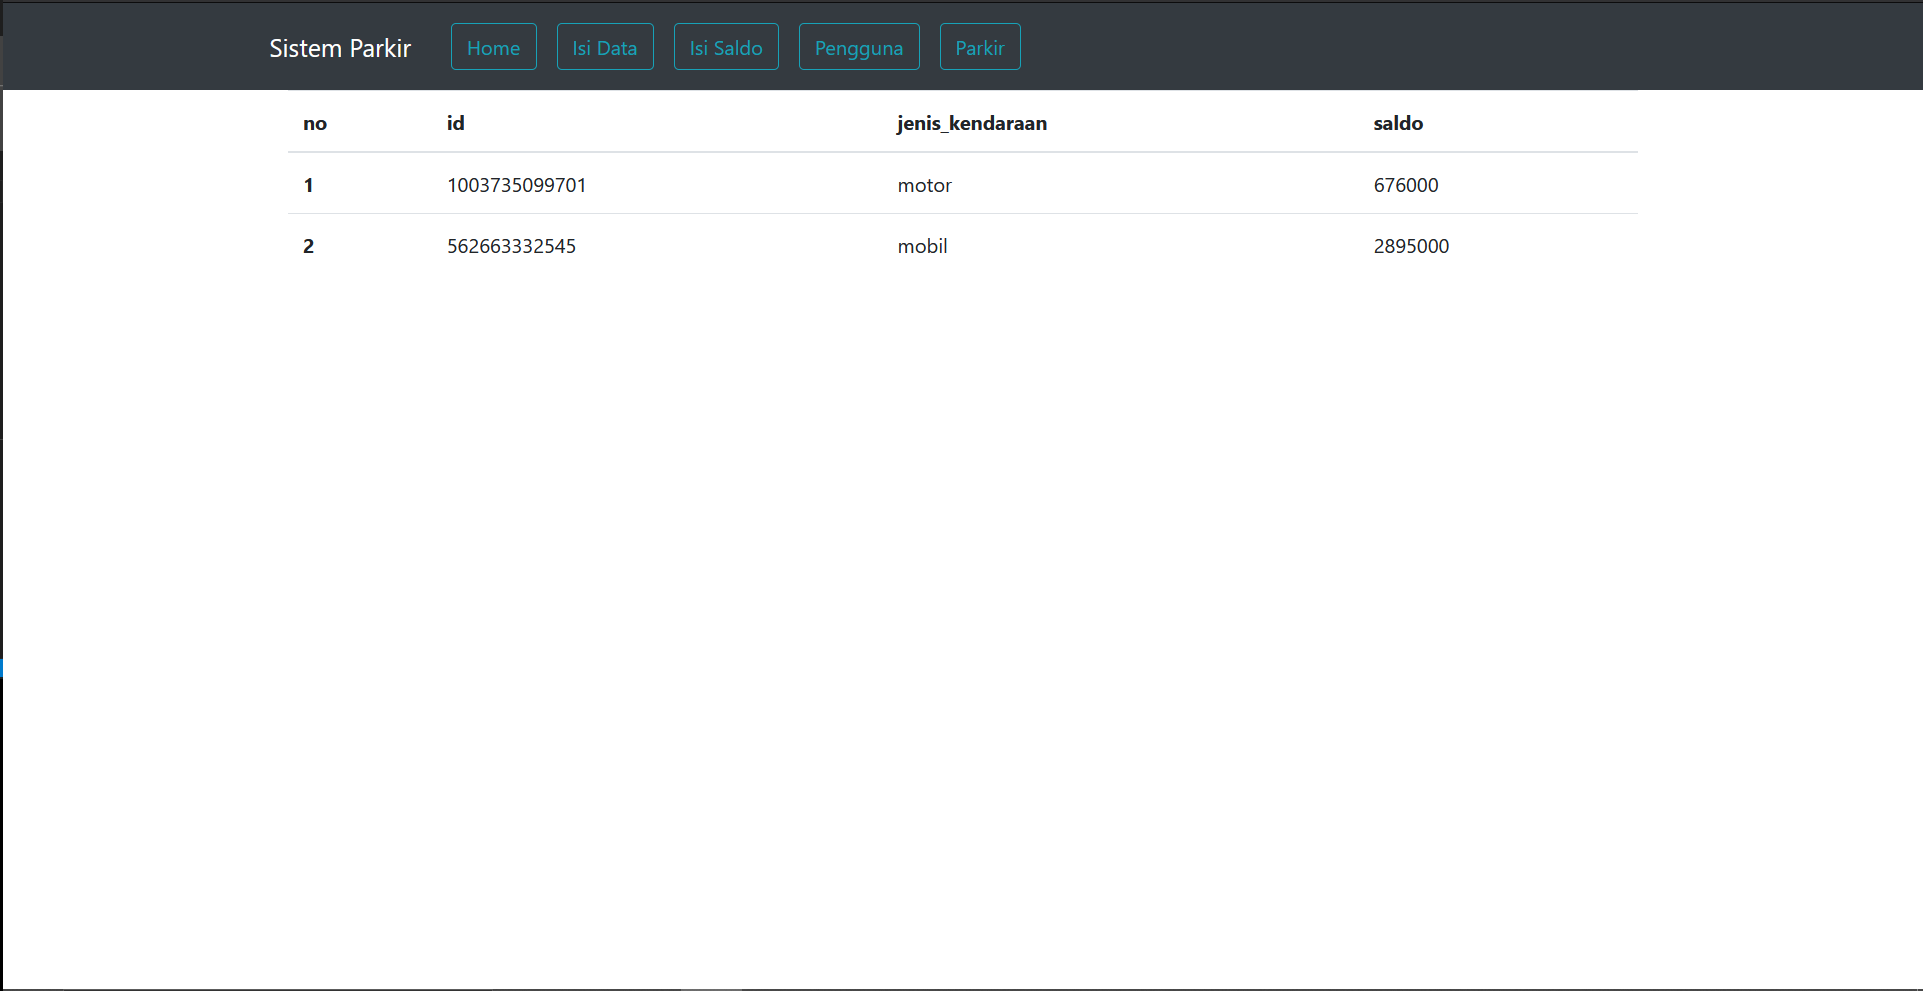
\includegraphics[width=0.85\textwidth, center]{images/web 4 pengguna.png}
    \caption{Daftar Pengguna}
    \label{fig:web4pengguna}
\end{figure}

Gambar ~\ref{fig:web4pengguna} merupakan gambar Tampilan Daftar Pengguna yang berfungsi untuk melihat pengguna yang telah terdaftar. Untuk mendaftarkan pengguna bisa dilakukan di \textit{Form} isi data.

\subsubsection{Tampilan Informasi}
\begin{figure} [H]
    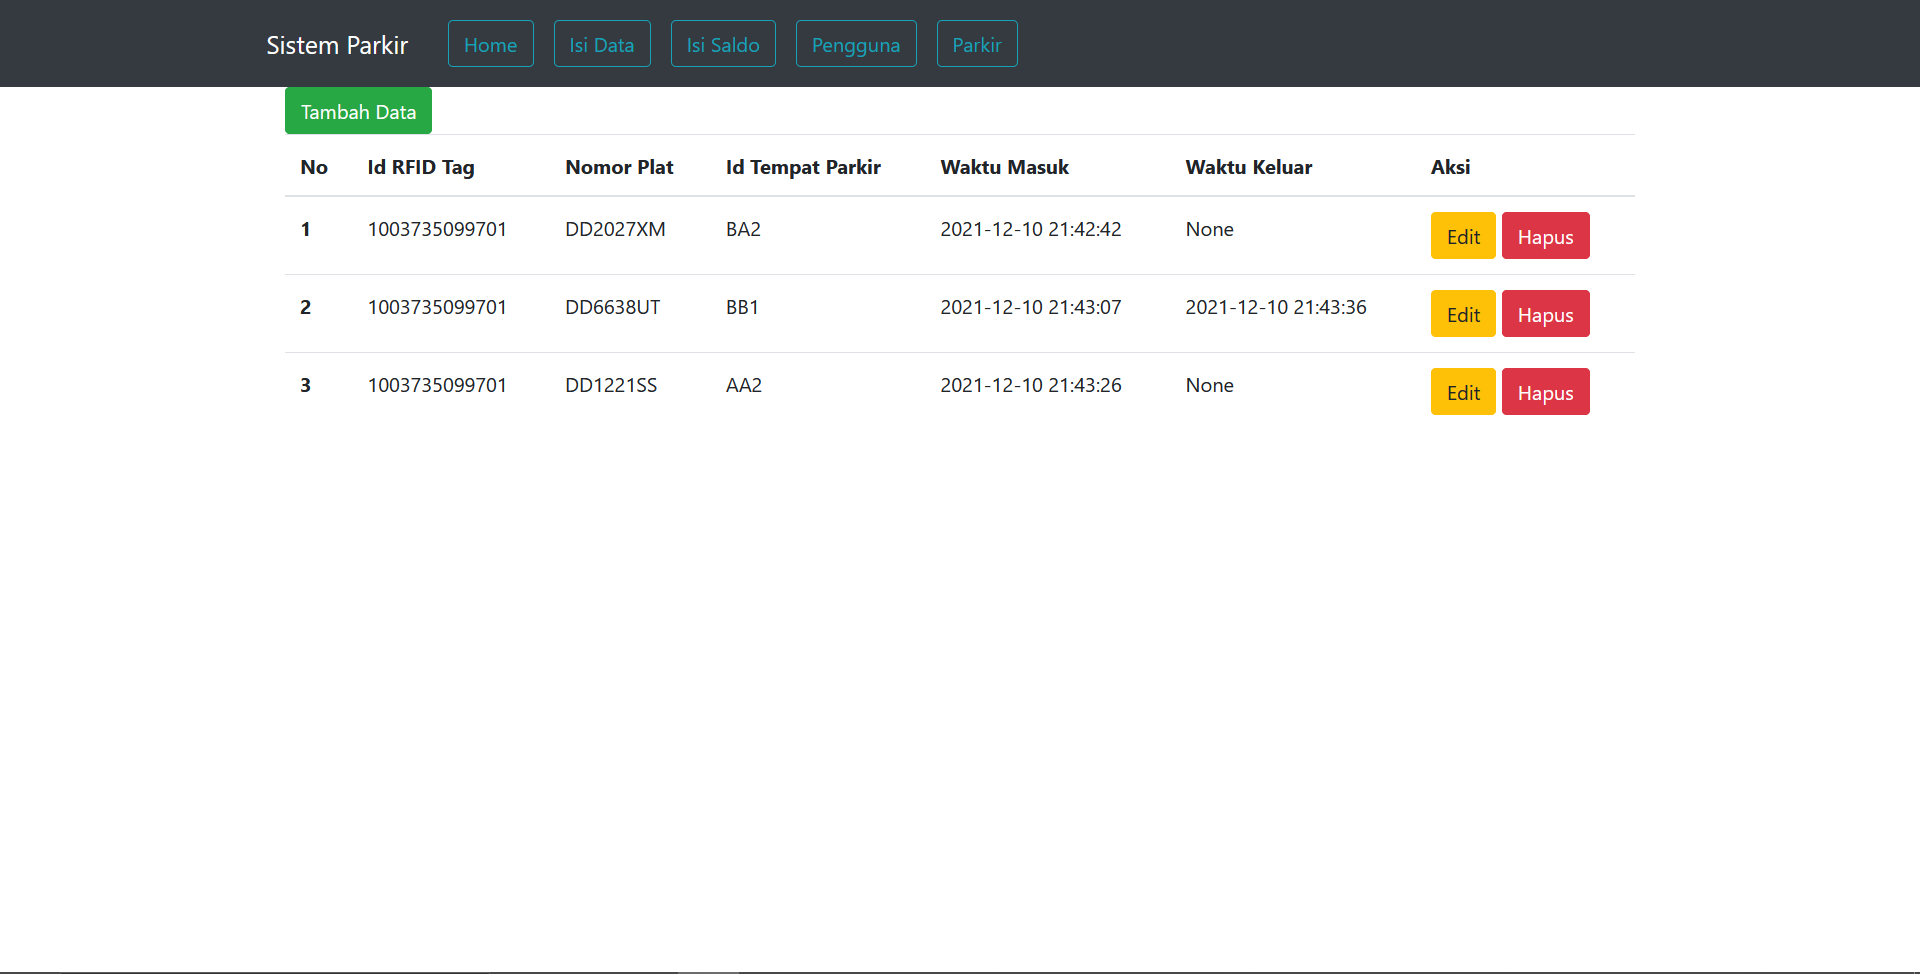
\includegraphics[width=0.85\textwidth, center]{images/web 5 informasi.png}
    \caption{Informasi}
    \label{fig:web5informasi}
\end{figure}

Gambar ~\ref{fig:web5informasi} merupakan gambar Tapilan Informasi yang brrfungsi untuk menampilkan informasi dari pengendara yang sedang parkir. Tampilan ini juga bisa digunakan sebagai tampilan \textit{history} karena manampilkan riwayat parkir semua pengendara. Pada tampilan ini juga terdapat \textit{button} untuk tambah data, edit data, dan hapus data.

\begin{figure} [H]
    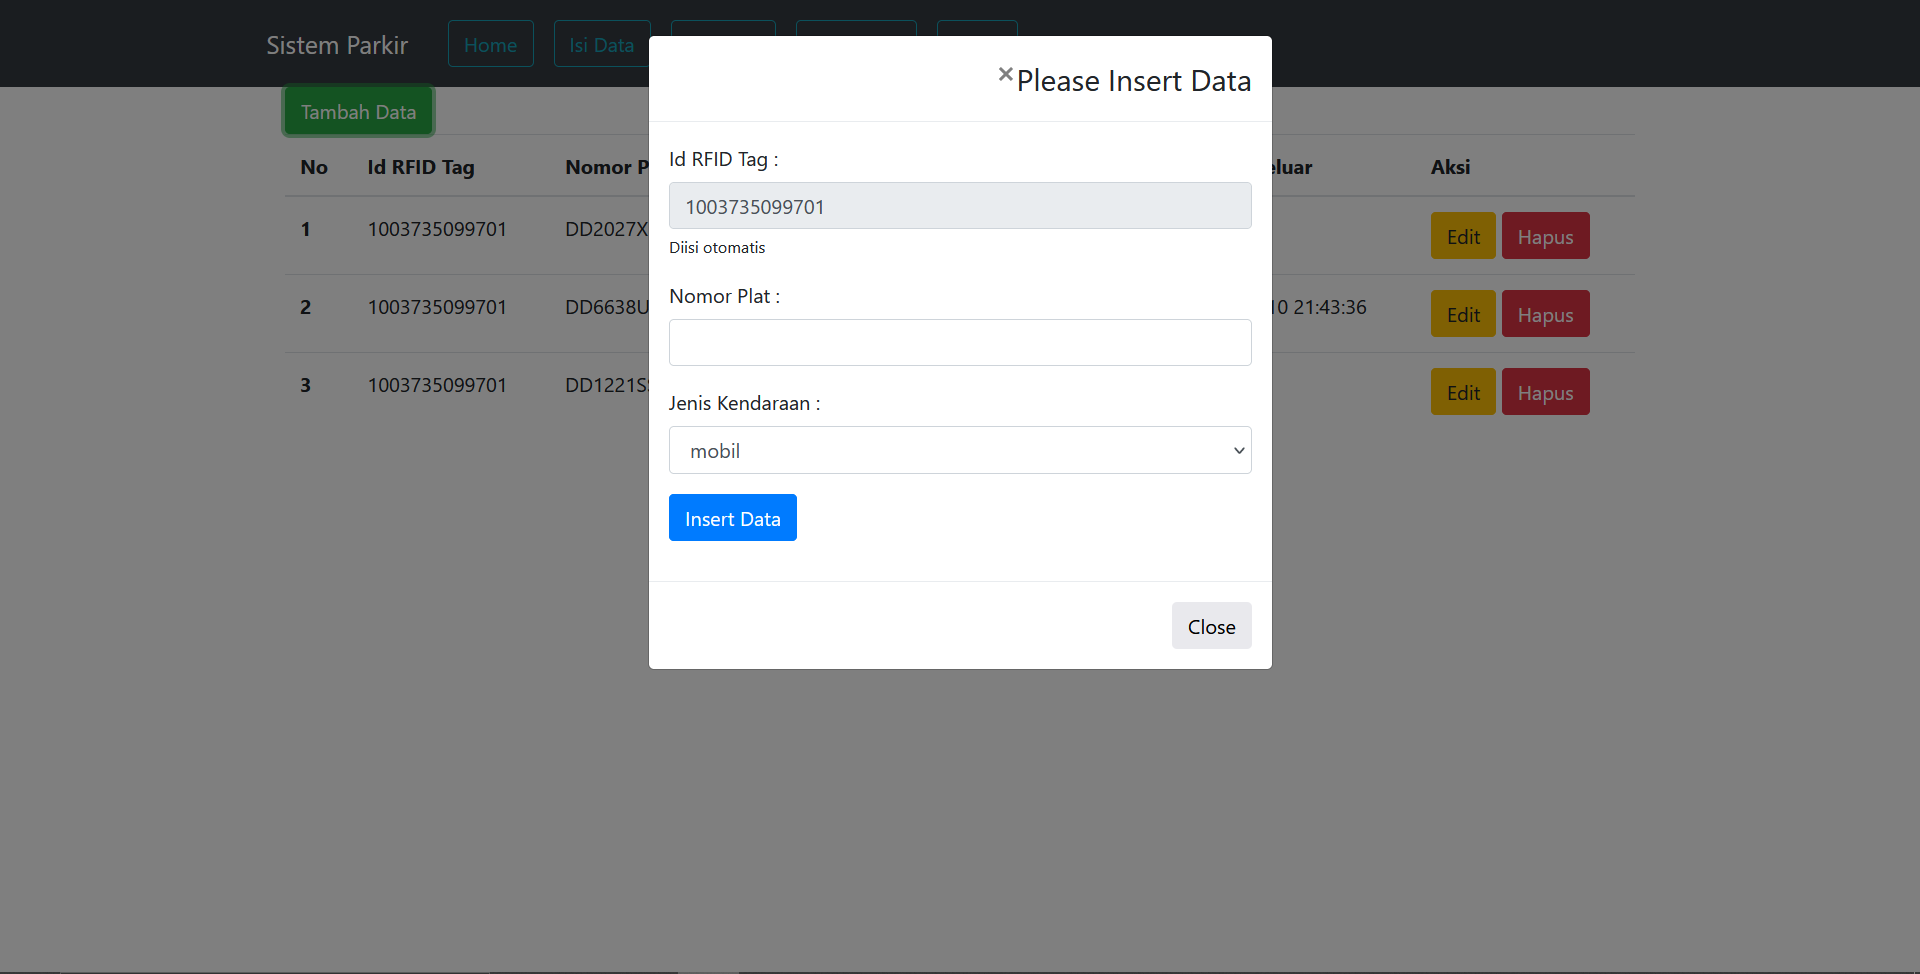
\includegraphics[width=0.85\textwidth, center]{images/web 5 tambah data.png}
    \caption{Tambah Data}
    \label{fig:web5tambahdata}
\end{figure}

Gambar ~\ref{fig:web5tambahdata} merupakan gambar tapilan yang muncul apabila \textit{button} tambah data ditekan. Pada tampilan ini terdapat \textit{form} untuk mengisi id rfid (diisi secara otomatis oleh sistem), nomor plat, dan jenis kendaraan.

\begin{figure} [H]
    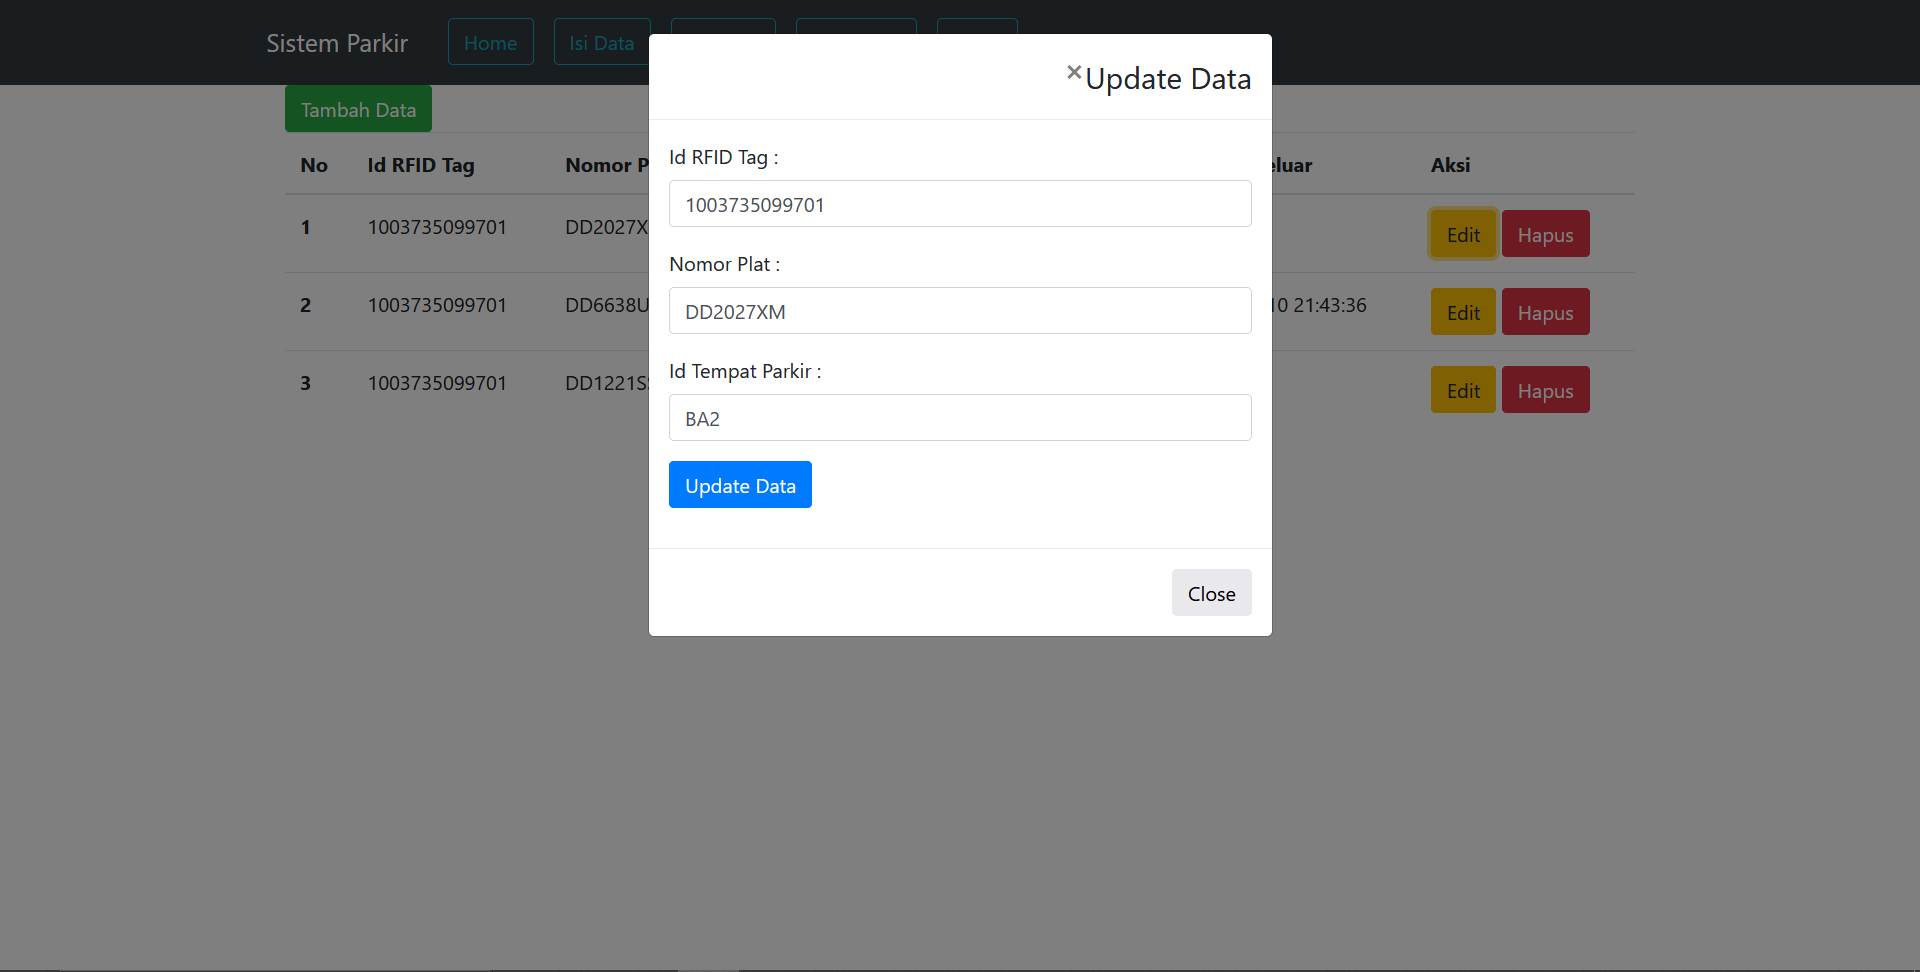
\includegraphics[width=0.85\textwidth, center]{images/web 5 edit data.png}
    \caption{Edit Data}
    \label{fig:web5editdata}
\end{figure}

Gambar ~\ref{fig:web5editdata} merupakan gambar tapilan yang muncul apabila \textit{button} edit data ditekan. Pada tampilan ini terdapat satu \textit{button} lagi yang apabila ditekan akan mengupdate waktu keluar.

\textit{Button} tambah data dan edit data baru akan digunakan apabila palang parkir tidak bisa terbuka karena nomor pelat tidak bisa di deteksi oleh sistem. Admin akan menekan \textit{push button} yang terdapat pada alat IoT untuk membuka paksa palang parkir agar kendaraan bisa masuk, kemudian admin akan menginput data kendaraan secara otomatis melalui \textit{button} tambah data pada tampilan informasi. \textit{Button} tambah data akan digunakan pada saat kendaraan akan masuk sedangkan \textit{button} edit data akan digunakan apabila nomor pelat tidak bisa di deteksi oleh sistem pada saat kendaraan akan keluar. \textit{Button update} data yang terdapat pada tampilan edit pada saat ditekan akan mengupdate variabel waktu keluar.
    \chapter{KESIMPULAN DAN SARAN}

\section{Kesimpulan}
Berdasarkan hasil penelitian yang diuraikan pada bab IV, maka peneliti menarik beberapa kesimpulan sebagai berikut :
\begin{enumerate}[topsep=0pt,itemsep=0pt,partopsep=0pt, parsep=0pt]
    \item Sistem identifikasi kendaran pada pemarkiran dengan pengenalan citra plat dan pembacaan rfid berhasil diimplementasikan. Rancangan alat yang dibuat masih bersifat \textit{prototype}. Adapun alat yang digunakan yaitu Raspberry Pi, RFID, ultrasonik, servo, dan kamera.
    \item Membuat aplikasi web sebagai \textit{user interface}. Web dibuat dengan bahasa pemrograman python dan flask sebagai \textit{framework}. Web yang dibuat memiliki beberapa fitur seperti melihat slot yang terisi dan tersedia, mendaftarkan pengguna baru, menambah saldo, dan melihat informasi mengenai slot parkir.
\end{enumerate}

\section{Saran}
Adapun saran yang diberikan kepada peneliti berikutnya apabila ingin mengembangkan penelitian ini agar menjadi lebih baik adalah sebagai berikut :
\begin{enumerate}[topsep=0pt,itemsep=0pt,partopsep=0pt, parsep=0pt]
    \item Melakukan penelitian dan analisis lebih lanjut pada deteksi nomor pelat kendaraan karena pada penelitian ini, peneliti masih menggunakan API dari pihak ketiga.
    \item Menambahkan fitur tambah slot parkir agar sistem parkir menjadi lebih fleksibel.
    \item Menambahkan sensor disetiap slot parkir untuk mengetahui apakah pengendara sudah parkir ditempat yang sudah ditentukan.
\end{enumerate}
    %-----------------------------------------------------------
    % End Daftar masukan untuk Bab
    %===========================================================

    %===========================================================
    % Daftar Pustaka
    %-----------------------------------------------------------
    \addcontentsline{toc}{chapter}{DAFTAR PUSTAKA}
    \printbibliography[title={DAFTAR PUSTAKA}]
    %-----------------------------------------------------------
    % End Daftar Pustaka
    %===========================================================
    
    %===========================================================
    % Daftar Lampiran
    %-----------------------------------------------------------
    \appendix
    \addcontentsline{toc}{chapter}{LAMPIRAN}
    \addtocontents{toc}{\protect\setcounter{tocdepth}{0}}
    \chapter*{LAMPIRAN}
\setcounter{chapter}{7}

% \newappendix{Source Code Program}

% \newappendix{Source Code Alat}

\newappendix{Source Code RFID}
\lstinputlisting[frame=single, style=python]{images/program/rfid.py}

\newappendix{Source Code Servo}
\lstinputlisting[frame=single, style=python]{images/program/servo.py}

\newappendix{Source Code Ultrasonik}
\lstinputlisting[frame=single, style=python]{images/program/ultra.py}

\newappendix{Source Code Kamera}
\lstinputlisting[frame=single, style=python]{images/program/kamera.py}

\newappendix{Source Code Main}
\lstinputlisting[frame=single, style=python]{images/program/main.py}

% \newappendix{Source Code Web}

\newappendix{Source Code Web}
\lstinputlisting[frame=single, style=python]{images/program/web.py}

% \begin{enumerate}[topsep=0pt,itemsep=0pt,partopsep=0pt, parsep=0pt]
%     \item RFID
%     \lstinputlisting[frame=single, style=python]{images/program/rfid.py}

%     \item Servo
%     \lstinputlisting[frame=single, style=python]{images/program/servo.py}

%     \item Ultrasonik
%     \lstinputlisting[frame=single, style=python]{images/program/ultra.py}

%     \item Kamera
%     \lstinputlisting[frame=single, style=python]{images/program/kamera.py}

%     \item Main
%     \lstinputlisting[frame=single, style=python]{images/program/main.py}

%     \item Web
%     \lstinputlisting[frame=single, style=python]{images/program/web.py}

% \end{enumerate}
    %-----------------------------------------------------------
    % End Daftar Lampiran
    %===========================================================

\end{document}